%%%%%%%%%%%%%%%%%%%%%%%%%%%%%%%%%%%%%%%%%%%%%%%%%%%%%%\sum_{j=1}^{n}%%%%%%%%%%%%%%%%%%%%%%%
%                                                                           %
%          LaTeX File for Doctor (Master) Thesis of ECNU                    %
%            华东师范大学博士(硕士)论文模板 ____lizb                        %
%                                                                           %
%%%%%%%%%%%%%%%%%%%%%%%%%%%%%%%%%%%%%%%%%%%%%%%%%%%%%%%%%%%%%%%%%%%%%%%%%%%%%
%!TEX program = xelatex
\documentclass[12pt,openany,a4paper,fancyhdr,oneside]{ctexbook}
%\documentclass[12pt,openright,a4paper,fancyhdr,twoside]{ctexbook}
%draft 选项可以使插入的图形只显示外框,以加快预览速度。
%\documentclass[11pt,a4paper,openany,draft]{book}

\usepackage{multirow}
\usepackage{listings}
\usepackage{xcolor}

\usepackage[CJKbookmarks,linkcolor=black,citecolor=black]{hyperref}
\usepackage{shortvrb,indentfirst,ulem,makeidx}
\usepackage{fancyhdr}
\usepackage{graphicx}
\usepackage{indentfirst,latexsym,amsthm,colortbl,subfigure,clrscode}
\usepackage{algorithm}
\usepackage{algorithmic}
\usepackage{bm}                     % 处理数学公式中的黑斜体的宏包
\usepackage{amsmath}                % AMSLaTeX宏包 用来排出更加漂亮的公式
\usepackage{amssymb}                % AMSLaTeX宏包 用来排出更加漂亮的公式
\usepackage{mathrsfs}
\usepackage[subnum]{cases}
\usepackage[numbers,sort&compress]{natbib}
%\usepackage[super,square,numbers,sort&compress]{natbib}
\usepackage{hypernat}
\usepackage{geometry}

\usepackage{times}
\usepackage{fontspec}
\usepackage{libertine}

\usepackage{caption}
\usepackage{titletoc}
\usepackage{titlesec}



\usepackage{inputenc}
\usepackage{listings}
\usepackage{color}
\usepackage{fontspec}

\usepackage{booktabs}%表格
\usepackage{colortbl}%表格虚线
\usepackage{arydshln}%表格虚线

\usepackage{multirow}%表格虚线
\usepackage{multicol}%表格虚线
\usepackage{diagbox} % 加载宏包
%\usepackage{url}%参考文献网址


\makeindex
\pagestyle{fancy}

\fancyhead[RO,LE]{\bfseries 华东师范大学研究生硕士学位论文}
\fancyhead[LO]{\small \leftmark} \fancyhead[RE]{\small \leftmark}

\renewcommand{\headrulewidth}{0.4pt}
\fancyfoot[CO,CE]{\thepage}

\renewcommand{\algorithmicrequire}{\textbf{Input:}}
\renewcommand{\algorithmicensure}{\textbf{Output:}}
\renewcommand{\algorithmiccomment}[1]{// #1}


%                    根据自己正文需要做的一些定义                 %
%==================================================================
\def\diag{{\rm diag}}
\def\rank{{\rm rank}}
\def\RR{{\cal R}}
\def\NN{{\cal N}}
\def\R{{\mathbb R}}
\def\C{{\mathbb C}}
\let\dis=\displaystyle

\def\p{\partial}
\def\f{\frac}
\def\mr{\mathrm}

\def\mb{\mathbf}
\def\mc{\mathcal}
\def\b{\begin}
\def\e{\end}

\newtheorem{thm1}{Theorem}[part]
\newtheorem{thm2}{Theorem}[section]
\newtheorem{thm3}{Theorem}[subsection]
\newtheorem{them}[thm2]{定理}
\newtheorem{theorem}[thm2]{定理}
\newtheorem{defn}[thm2]{定义}
\newtheorem{define}[thm2]{定义}
\newtheorem{ex}[thm2]{例}
\newtheorem{exs}[thm2]{例}
\newtheorem{example}[thm2]{例}
\newtheorem{prop}[thm2]{命题}
\newtheorem{lemma}[thm2]{引理}
\newtheorem{cor}[thm2]{推论}
\newtheorem{remark}[thm2]{注释}
\newtheorem{notation}[thm2]{记号}
\newtheorem{abbre}[thm2]{缩写}
% \newtheorem{algorithm}[thm2]{算法}
\newtheorem{problem}[thm2]{问题}

\newcommand{\tabincell}[2]{\begin{tabular}{@{}#1@{}}#2\end{tabular}}

\newcommand{\yihao}{\fontsize{26pt}{36pt}\selectfont}           % 一号, 1.4 倍行距
\newcommand{\erhao}{\fontsize{22pt}{28pt}\selectfont}          % 二号, 1.25倍行距
\newcommand{\xiaoer}{\fontsize{18pt}{18pt}\selectfont}          % 小二, 单倍行距
\newcommand{\sanhao}{\fontsize{16pt}{24pt}\selectfont}        % 三号, 1.5倍行距
\newcommand{\xiaosan}{\fontsize{15pt}{22pt}\selectfont}        % 小三, 1.5倍行距
\newcommand{\sihao}{\fontsize{14pt}{21pt}\selectfont}            % 四号, 1.5 倍行距
\newcommand{\banxiaosi}{\fontsize{13pt}{19.5pt}\selectfont}    % 半小四, 1.5倍行距
\newcommand{\xiaosi}{\fontsize{12pt}{18pt}\selectfont}            % 小四, 1.5倍行距
\newcommand{\dawuhao}{\fontsize{11pt}{11pt}\selectfont}       % 大五号, 单倍行距
\newcommand{\wuhao}{\fontsize{10.5pt}{15.75pt}\selectfont}    % 五号, 单倍行距



%============================ 可以自定义文字块 ================================%

\newcommand{\aaa}{这是我给你们的一个示例}
\newcommand{\bbb}{\aaa \aaa \aaa}
\newcommand{\ccc}{\bbb \bbb \bbb \bbb \bbb

\bbb \bbb \bbb \bbb \bbb }
\newcommand{\abc}{abcdefg1234567890}
\newcommand{\upabc}{ABCDEFGHIJK}
%%% ----------------------------------------------------------------------
\newenvironment{myfont}{\fontfamily{lmtt}\selectfont}{\par}
\DeclareTextFontCommand{\textmyfont}{\myfont}

\newfontfamily\courier{Courier New}

%============================= 版芯控制 ================================%
\setlength{\oddsidemargin}{0.57cm}
\setlength{\evensidemargin}{\oddsidemargin}
\voffset-6mm \textwidth=150mm \textheight=230mm \headwidth=150mm
%\rightmargin=35mm
%                                                                       %


%============================= 页面设置 ================================%
%-------------------- 定义页眉和页脚 使用fancyhdr 宏包 -----------------%
% 定义页眉与正文间双隔线
\newcommand{\makeheadrule}{%
\makebox[0pt][l]{\rule[.7\baselineskip]{\headwidth}{0.4pt}}%
\rule[0.85\baselineskip]{\headwidth}{0.4pt} \vskip-.8\baselineskip}
\makeatletter
\renewcommand{\headrule}{%
{\if@fancyplain\let\headrulewidth\plainheadrulewidth\fi
\makeheadrule}} \makeatother

\newcommand{\upcite}[1]{\textsuperscript{\textsuperscript{\cite{#1}}}}

\newcommand{\adots}{\mathinner{\mkern 2mu%
\raisebox{0.1em}{.}\mkern 2mu\raisebox{0.4em}{.}%
\mkern2mu\raisebox{0.7em}{.}\mkern 1mu}}

%\setmainfont{Times New Roman}
\dottedcontents{chapter}[1.5cm]{\xiaosi\heiti}{3.8em}{9.5pt}
\dottedcontents{section}[1.5cm]{\xiaosi\heiti}{2.8em}{9.5pt}




%=============================== 代码展示设置 ================================%

\definecolor{codegreen}{rgb}{0,0.6,0}
\definecolor{codegray}{rgb}{0.5,0.5,0.5}
\definecolor{codepurple}{rgb}{0.58,0,0.82}
\definecolor{backcolour}{rgb}{0.95,0.95,0.92}

%Code listing style named "mystyle"
\lstdefinestyle{mystyle}{
  backgroundcolor=\color{backcolour},
  commentstyle=\color{codegreen},
  keywordstyle=\color{magenta},
  numberstyle=\tiny\color{codegray},
  stringstyle=\color{codepurple},
  basicstyle=\small\courier,
  breakatwhitespace=false,
  breaklines=true,
  captionpos=b,
  keepspaces=true,
  numbers=left,
  numbersep=5pt,
  showspaces=false,
  showstringspaces=false,
  showtabs=false,
  tabsize=2
}

\lstset{style=mystyle}

%=============================== 正文部分 ================================%


\begin{document}

 \pagestyle{empty}
\setlength{\baselineskip}{25pt}  %%正文设为25磅行间距
\vspace{-2.0cm}
\noindent{{\zihao{4} {\large 2022} 届硕士专业学位研究生学位论文}}\\
\vspace{-0.8cm}
\begin{flushleft}
\hspace{-0.5cm}
\renewcommand\arraystretch{1.5}
\begin{tabular}{l}
\noindent{{\zihao{4} 分类号:\underline{\qquad\qquad\qquad\qquad\qquad\qquad}}}  \\
\noindent{{\zihao{4} 密~~~~级:\underline{\qquad\qquad\qquad\qquad\qquad\qquad}}}\\
\end{tabular}
\hskip 1.1cm
\renewcommand\arraystretch{1.5}
\begin{tabular}{l}
\noindent{{\zihao{4} 学校代码:\underline{10269~~~\qquad}}}\\
\noindent{{\zihao{4} 学~~~~~~~~号:\underline{51194501126}}}\\
\end{tabular}
\end{flushleft}


\vskip 1.0cm

\begin{center}
	\hskip 0.5cm
	\scalebox{1.0}{
\includegraphics[width=2.7cm]{fig/ecnulogo.png}}
	\scalebox{1.0}{
\includegraphics[width=11.5cm,height=2.7cm]{fig/ecnulabel.png}}
	\vskip 0.5cm
	{\textbf{{\xiaoer East China Normal University}}}\\ \vskip 0.2cm
	{\textbf{\erhao 硕~士~专~业~学~位~论~文}}\\ \vskip 0.2cm
	{\textbf{{\xiaoer MASTER'S DISSERTATION (Professional)}}}\\\end{center}





\vskip 1.0cm

\begin{center}
{\zihao{2}\bf 论文题目:联邦学习中差分隐私和安全混洗的研究}
\end{center}

\vskip 1.0cm
\begin{center}

\renewcommand\arraystretch{1.5}
	\begin{tabular}{l}
{\sihao \bf 院\qquad\ \ 系:}\\
{\sihao \bf 专业学位类别:}\\
{\sihao \bf 专业学位领域:}\\
{\sihao \bf 论文指导教师:}\\
{\sihao \bf 论~文~作~者:}
\end{tabular}
\begin{tabular}c
{\sihao \bf  ~~软件工程学院}               \\
\hline {\sihao \bf ~~工程硕士 }              \\
\hline {\sihao \bf ~~软件工程~~}\\
\hline \bf ~~曹珍富\  教授  \\
% \hline ~~\    \\%盲审版本
\hline \bf ~~何慧娴\   \\
% \hline ~~\   \\%盲审版本
\hline
\end{tabular}


\end{center}

\vskip 2.0cm
\begin{center}
{\sihao 2021年09月10日}
\end{center}

 %\clearpage\ \newpage
 \newpage

\pagestyle{empty}

\noindent{Thesis (Professional) for Master’s Degree in 2021}
\hskip 1.4cm {School Code: \underline{10269~~~~~~~~~~~\qquad}}\\
\hspace*{\fill} {Student Number:\underline{51194501126~~~~~~~~}}
\vskip 2cm

\begin{center}
{\Huge \bf EAST\,CHINA\,NORMAL\,UNIVERSITY}
\end{center}

\vskip 3cm

\begin{center}
{\huge \bf \scshape Title: Technologies research for privacy preserving based on federated learning}
\end{center}

\vskip 2cm {\large
\begin{center}
\begin{tabular}{l}
Department:\\
			\\
Major:\\
Research Direction:\\
Supervisor:\\
Candidate:
\end{tabular}
\begin{tabular}c
~~~Software Engineering Institute\\
\hline ~~~Software Engineering  \\
\hline ~~~Privacy Preserving\\
\hline ~~~Professor ~ZhenFu Cao~  \\
%\hline ~~~  \\%盲审版本
\hline ~~~HuiXian He  \\
%\hline ~~~  \\%盲审版本
\hline
\end{tabular}
\end{center}}

\vskip 30mm

\begin{center}
{\Large Nov 9, 2021}
\end{center}

 %\clearpage\ \newpage
 % \newpage
\pagestyle{empty}
\centerline{\bf\Large 华东师范大学学位论文原创性声明}

\vskip 0.85cm

%\normalsize \indent
%郑重声明:本人呈交的学位论文《{\color{red}基于SMT技术的机器学习树模型的鲁棒性的验证与分析}》,是在华东师范大学攻读硕士/博士(请勾选)学位期间,在导师的指导下进行的研究工作及取得的研究成果。除文中已经注明引用的内容外,本论文不包含其他个人已经发表或撰写过的研究成果。对本文的研究做出重要贡献的个人和集体,均已在文中作了明确说明并表示谢意。
$$\\  $$

%\qquad\qquad{作者签名}:彭宏伟
%\qquad\qquad\qquad \mbox {日期}:\quad 2018 年 6月14日

%\qquad\qquad{作者签名}: \quad 
%\qquad\qquad\qquad \mbox {日期}:\qquad\qquad  年 \qquad  月\qquad   日

%\vskip 0.85cm

%\centerline{\bf\Large 华东师范大学学位论文著作权使用声明}

%\vskip 0.85cm

%《{\color{red}基于SMT技术的机器学习树模型的鲁棒性的验证与分析}》系本人在华东师范大学攻读学位期间在导师指导下完成的硕士/博士(请勾选)学位论文,本论文的研究成果归华东师范大学所有。本人同意华东师范大学根据相关规定保留和使用此学位论文,并向主管部门和相关机构如国家图书馆、中信所和“知网”送交学位论文的印刷版和电子版;允许学位论文进入华东师范大学图书馆及数据库被查阅、借阅;同意学校将学位论文加入全国博士、硕士学位论文共建单位数据库进行检索,将学位论文的标题和摘要汇编出版,采用影印、缩印或者其它方式合理复制学位论文。

%本学位论文属于(请勾选)

%(  )1.经华东师范大学相关部门审查核定的“内部”或“涉密”学位论文*,
%于     年    月    日解密,解密后适用上述授权。

%(  )2.不保密,适用上述授权。
%$$\\ $$
%\qquad\qquad \mbox{导师签名}: 王晓玲
%\qquad\qquad \mbox {本人签名}: 彭宏伟

%\qquad\qquad \mbox{导师签名}: \quad 
%\qquad\qquad \mbox {本人签名}: \quad 

%\vskip 0.85cm

%$\rightline{ \qquad 2018 年  6 月  14 日 \qquad\qquad}$
%$\rightline{ \qquad  年 \qquad  月 \qquad  日 \qquad\qquad}$

%\vskip 0.85cm

%* “涉密”学位论文应是已经华东师范大学学位评定委员会办公室或保密委员会审定过的学位论文(需附获批的《华东师范大学研究生申请学位论文“涉密”审批表》方为有效),未经上述部门审定的学位论文均为公开学位论文。此声明栏不填写的,默认为公开学位论文,均适用上述授权)。

 %\clearpage\ \newpage
 % \newpage
\pagestyle{empty}
$$\\ \\ \\ $$

\centerline{\bf\Large $\underline{\mbox{\kaishu {XXX}}}\,\,
	$硕士学位论文答辩委员会成员名单}

\vskip 10mm

\begin{center}
	{\large
		\begin{tabular}{| p{25mm}| p{30mm}| p{64mm}| p{23mm}|}\hline
			\vfill\hfill{\heiti 姓名}\hspace*{\fill} &\vfill\hfill{\heiti 职称}\hspace*{\fill} &
			\vfill\hfill{\heiti 单位}\hspace*{\fill} &\vfill\hfill {\heiti 备注~~~~~} \hspace*{\fill} \\[6pt]\hline
			\vfill\hfill{\kaishu }\hspace*{\fill} &\vfill\hfill{\kaishu }\hspace*{\fill} &\vfill\hfill{\kaishu }\hspace*{\fill} & \vfill\hfill {\kaishu ~~~~~~}\hspace*{\fill} \\[6pt]\hline
			\vfill\hfill{\kaishu }\hspace*{\fill} &\vfill\hfill{\kaishu }\hspace*{\fill} &\vfill\hfill{\kaishu \tabincell{c}{} }\hspace*{\fill} & \vfill{\heiti }\\[20pt]\hline
			\vfill\hfill{\kaishu }\hspace*{\fill} &\vfill\hfill{\kaishu }\hspace*{\fill} &\vfill\hfill{\kaishu }\hspace*{\fill} & \vfill{\heiti }\\[20pt]\hline
			%\vfill\hfill{\kaishu ~~~}\hspace*{\fill} &\vfill\hfill{\kaishu ~~~}\hspace*{\fill} &\vfill\hfill{\kaishu ~~~}\hspace*{\fill} & \vfill{\heiti }\\[20pt]\hline
%			\vfill\hfill{\kaishu ~~~}\hspace*{\fill} &\vfill\hfill{\kaishu ~~~}\hspace*{\fill} &\vfill\hfill{\kaishu ~~~}\hspace*{\fill} & \vfill{\heiti }\\[20pt]\hline
%			\vfill\hfill{\kaishu ~~~}\hspace*{\fill} &\vfill\hfill{\kaishu ~~~}\hspace*{\fill} &\vfill\hfill{\kaishu ~~~}\hspace*{\fill} & \vfill{\heiti }\\[20pt]\hline
			%              &             &              &  \vfill{\heiti }\\[20pt]\hline
		\end{tabular}
	}
\end{center}


\clearpage\ \newpage

\newpage
\pagenumbering{roman}
\pagestyle{plain}
\vspace{-2.5cm}
\chapter*{\zihao{2}\heiti{摘~~~~要}}
%\vskip 1cm
%\vspace{-1cm}

随着数据孤岛的出现和隐私意识的普及,联邦学习作为一种新兴的数据共享和交换模型在金融、医疗、教育等诸多领域得到广泛应用。联邦学习的基本框架包含多个本地设备和一个中央服务器,所有训练数据保存在本地设备,所有设备共同协作训练一个全局模型。联邦学习的一个突出优点是它可以在服务器和客户端之间无需任何个人数据交换的情况下进行本地训练。但是,联邦学习也存在各种安全和隐私问题。近年来,大量的研究结果表明,联邦学习机制仍然存在安全问题,在训练过程中,本地设备与中央服务器之间的通信信道和传递的模型参数都有可能成为第三方窃取敏感信息的途径,联邦学习仍然面临各种安全和隐私威胁。针对联邦学习中用户本地训练数据、模型参数、模型架构等隐私的攻击方式包括投毒攻击、模型重建攻击、模型反演攻击、成员推理攻击等。

随着针对联邦学习框架的攻击模型增多,研究人员开始关注训练联邦学习模型时存在的隐私安全问题。针对联邦学习中的隐私保护的技术主要分为两类,一类是基于密码学技术,比如安全多方计算、同态加密等;另一类是基于系统安全技术,包括差分隐私、匿名技术、安全混洗等。基于安全多方计算的联邦学习隐私保护技术主要是在联邦学习中应用不经意传输、混淆电路、秘密共享等技术达到隐私保护的目的;基于同台加密的联邦学习隐私保护技术主要是通过加法同态、乘法同态或者全同态加密技术对用户上传的参数进行加密,以防止中央服务器或者恶意第三方服务器的攻击。虽然这两种密码学技术对数据的隐私保护效果很好,但应用于实际的联邦学习环境中,会出现模型难以收敛、计算成本过高、通信效率降低等问题,这阻碍了隐私保护的深度神经网络在当今工业中的全面应用,也是研究领域中尚未解决的一个争论。而差分隐私等系统安全技术却在模型精度、通信效率上能达到更好的效果。因此,本文主要是基于系统安全技术对联邦学习中的隐私保护问题进行研究。

当前在联邦学习模型中应用差分隐私的主流方案是在本地训练随机梯度下降过程中,在梯度上添加噪声。Song等人\upcite{ref47}提出了一个$\left(\epsilon_{c}+\epsilon_{d}\right)$-差分隐私版本的随机梯度下降算,在本地模型的每一次迭代过程中,对梯度添加高斯噪声,并通过差分隐私的组合性和隐私放大效果,得到完全隐私损失的上界。差分隐私随机梯度下降 (DP-SGD) 严重降低了训练模型的效用,在数据集上训练和验证的损失率大大增加。因此本文针对模型效用和数据隐私保护的双重目标,设计、实现并评估了一个实用的联邦学习系统,该系统在保护数据隐私的前提下尽可能的维持了模型的精度和通信效率。本文主要的工作和贡献如下:

\begin{enumerate}
\item [(1)] 在联邦学习差分隐私的场景下,本文设计了一种新型的、基于本地差分隐私的权重分配自适应干扰算法和梯度自适应裁剪算法。首先,我们考虑到不同的深度神经网络(DNN)层的模型权重可能会有很大的变化,提出了一种基于权重的贡献率添加自适应噪声的算法:在客户端本地训练的神经网络模型中,通过分析前向传播算法,计算每个属性类对于模型输出的贡献比,根据梯度的贡献率注入不同隐私预算的噪声。

\item [(2)]在传统的差分隐私随机梯度下降算法中,通常采用固定的裁剪阈值对梯度进行裁剪以限制函数的敏感度,然而固定的梯度裁剪可能添加额外的噪声。本文设计了一种自适应调整剪裁阈值的方案,通过计算梯度更新的方差和偏差,逐元素地对梯度进行裁剪,与之前的方案相比,通过使用梯度的坐标自适应剪裁实现了相同的隐私保证,而增加的噪声要少得多。之后我们利用“Moments Accountant”机制分析加噪累积产生的隐私预算,并证明了我们的方案满足$\left(\epsilon_{c}+\epsilon_{l}\right)$-差分隐私。与传统的注入噪声的方法相比,我们在相同的隐私保护程度下大大减少了噪声对模型输出结果的影响,提高了模型的准确性。

\item [(3)]由于本地差分隐私并不能有效防御针对联邦学习的生成对抗网络攻击,并且在通信轮数较大的联邦学习模型中,本地自适应差分隐私的强组合性质会导致总体隐私预算过高。本文提出了一种新的安全聚合机制,在本地客户端和中央服务器之间新增安全混洗器,在用户将参数上传到云服务器之前,先对参数进行拆分混洗,模型参数的更新被匿名的发送到混洗器,通过对模型参数的拆分和混洗实现客户端匿名,并减轻由联邦学习模型的高数据维度和大量查询迭代引起的隐私预算爆炸问题。

\item [(4)]为了验证本文的方案在实际生产环境中的可行性,本文模拟了联邦学习环境,分别在MNIST、CIFAR-10、FMNIST三种数据集上进行实验,首先通过控制变量法分析各个参数对于模型精度的影响和隐私保护的效用,并与前人的差分隐私方案和安全混洗方案进行对比,通过实验结果证明了自适应本地差分隐私方案和安全混洗框架的结合,在较低的隐私预算下还能使联邦学习模型维持较高的精度。
\end{enumerate}
\hspace{-0.5cm}
\sihao{\heiti{关键词:}} \xiaosi{联邦学习,隐私保护,差分隐私,安全混洗}

 %\clearpage\ \newpage
\newpage
\vspace{-1cm}
\chapter*{\zihao{-2}\heiti{ABSTRACT}}
%\vspace{-0.5cm}

With the rapid development of artificial intelligence and the proliferation of mobile devices, application scenarios that require the collaboration of multiple participants are emerging.The role of distributed data processing and distributed machine learning is becoming increasingly prominent. For example, financial data scattered across multiple banks, medical records in different hospitals, behavioural records of each user under a large platform, as well as data generated by smart meters, sensors or mobile devices all need to be processed and mined in a distributed manner. 

Data silos are one of the key challenges that distributed data processing and distributed machine learning facing. As a solution to address data silos, Federated Learning is a promising distributed computing framework that can train models locally on multiple decentralised edge devices without transferring their data to servers. With the increasing awareness of privacy among citizens and the improvement of related laws, privacy security in federation learning is also a growing concern, and recent research work has shown that it has been possible to restore users' private data by attacking the gradient parameters of the model, i.e. it is not enough to protect privacy by keeping the data local, and privacy-preserving techniques just protect privacy at the huge expense of model accuracy. 

To this end, this paper uses differential privacy techniques to protect the privacy of users in federated learning, and analyses the adaptive interference mechanism against the gradient descent algorithm during model training for distributed scenarios.In order to achieve the goal of improving model accuracy, we propose a secure split-shuffle model to prevent attacks by malicious servers. 

The main work of this paper includes the following aspects:

\begin{enumerate}
	\item In a federated learning differential privacy scenario, this paper presents a novel, local adaptive differential privacy interference algorithm. In a client-side locally trained neural network model, the contribution ratio of each attribute class to the model output is calculated by analysing the forward propagation algorithm, and then we develop an adaptive noise addition scheme that injects noise with different privacy budgets according to the contribution ratio. Compared with the traditional method of injecting noise, we maximise the accuracy of the model with the same degree of privacy protection, reduce the impact of noise on the model output results and improve the model accuracy.
	\item Considering the attacks on parameter aggregators in federated learning, this paper proposes a new secure aggregation mechanism by adding a new shuffler between the local client and the central server, where parameters are splitted and shuffled before users upload them to the cloud server. The updates to model parameters are sent anonymously to the shuffler, achieving client anonymity through splitting and shuffling of model parameters.Finally, we demonstrate the feasibility of the shuffle model.
	\item In this paper, we do experiments on three datasets,then demonstrate the combination of the local adaptive differential privacy algorithm and the secure shuffle framework can reach the balance between model accuracy and privacy in the federated learning model.
\end{enumerate}
%\hspace{-0.5cm}
{\sihao{\textbf{Keywords:}}} \textit{Federated learning, Privacy preserving, Differential privacy , Security shuffle}



\clearpage\ \newpage
\setcounter{tocdepth}{2}

\tableofcontents
\listoffigures
\listoftables
\listofalgorithms

\newpage
\pagenumbering{arabic}
\pagestyle{fancy}

\CTEXsetup[format+={\zihao{3}\heiti}]{chapter}
\CTEXsetup[format+={\raggedright\zihao{4}\heiti}]{section}
\CTEXsetup[format+={\zihao{-4}\heiti}]{subsection}


\setlength{\baselineskip}{25pt}  %%正文设为25磅行间距


\chapter{绪\hskip 0.4cm 论}
\label{ch1}

\section{研究背景}
在过去的近十年,人工智能(Artificial Intelligence,AI)取得了令人难以置信的进步,广泛地应用于各种领域。为了进一步提高模型的训练精度和学习能力,新兴的深度神经网络,也称为深度学习(Deep Learning,DL)随之提出,深度学习凭借其高效的数据建模、抽象和泛化能力大幅提升了模型的预测准确率。深度学习算法的目标是通过从数据中泛化来学习如何执行某些任务,作为最有前景的技术之一,已广泛应用于图像分类、自动驾驶、智慧医疗等各个方面。例如,智能图像识别系统已广泛部署在机场、火车站等公共场所,用于识别可疑恐怖分子和检测违禁物品;基于深度学习的回归技术还可以帮助诊断和预防某些疾病;基于卷积神经网络实现无人驾驶车辆系统的目标检测和自动决策等。

当前深度学习的商业应用模式可以概括为:各个信息机构通过其提供的服务平台从用户处收集数据,训练算法模型以提升服务质量,从而获得更多的用户量和数据量。用户的搜索记录、浏览历史、购买交易、观看的视频都有可能被各个商业机构收集,用作模型训练的数据集。在2018年,中国互联网协会收到用户举报,发现腾讯等多家应用软件以“通过深度学习向用户提供更好的服务”为由,长期收集并保存大量的用户个人数据,如照片、地址、电话等。人们开始担心自己的数据被收集后会被泄露或者是被不正当使用。2018年欧盟也正式颁布实施了《通用数据保护法案》,旨在保护用户的个人隐私和数据安全。

深度学习提供的服务以大数据算法为基础,然而多个数据源之间也存在着难以打破的壁垒。在大多数行业中,数据是以孤立的岛屿形式存在的。例如,某机构基于深度学习的算法提供商品推荐的服务,它拥有用户的基本信息数据,却缺失了关于用户消费水平和购买偏好的数据,没有用户购物相关的特征难以训练出精准的推荐数据。除了一些巨头公司,绝大多数的企业存在数据质量差、数据量少的问题,使得他们难以提供优质的人工智能服务。如何在符合法律法规的前提下,采用跨组织的数据进行模型训练,并保护用户的隐私和数据安全是一大难题。

针对数据孤岛问题,Google在2016年提出了联邦学习的框架,它是一种有助于解决多方计算下的数据孤岛问题的学习方法。如图\ref{fig:联邦学习模型概况}所示,联邦学习的基本框架包含多个本地设备和一个中央服务器,所有训练数据保存在本地设备,不同的参与方按照各自的需求在本地训练模型更新权重。中央服务器接收所有本地设备上传的模型权重,训练一个全局的虚拟模型,通过将各方数据以共享梯度的方式进行聚合,更新全局参数。然后本地设备再从中央服务器下载全局参数,迭代地进行更新,使模型的训练结果最优化。联邦学习本质上是深度学习和分布式计算的结合,将模型训练与在云中存储数据的需求相分离,在合法合规的基础上,使所有本地设备可以在不共享训练数据的情况下联合建模。与集中式深度学习相比,联邦学习系统通过分布式的多方协作学习破解了数据孤岛的壁垒,实现更智能的模型、更低的延迟和更少的功耗,在学术界和工业界受到广泛关注。

\begin{figure}[!hbt]
\centering
	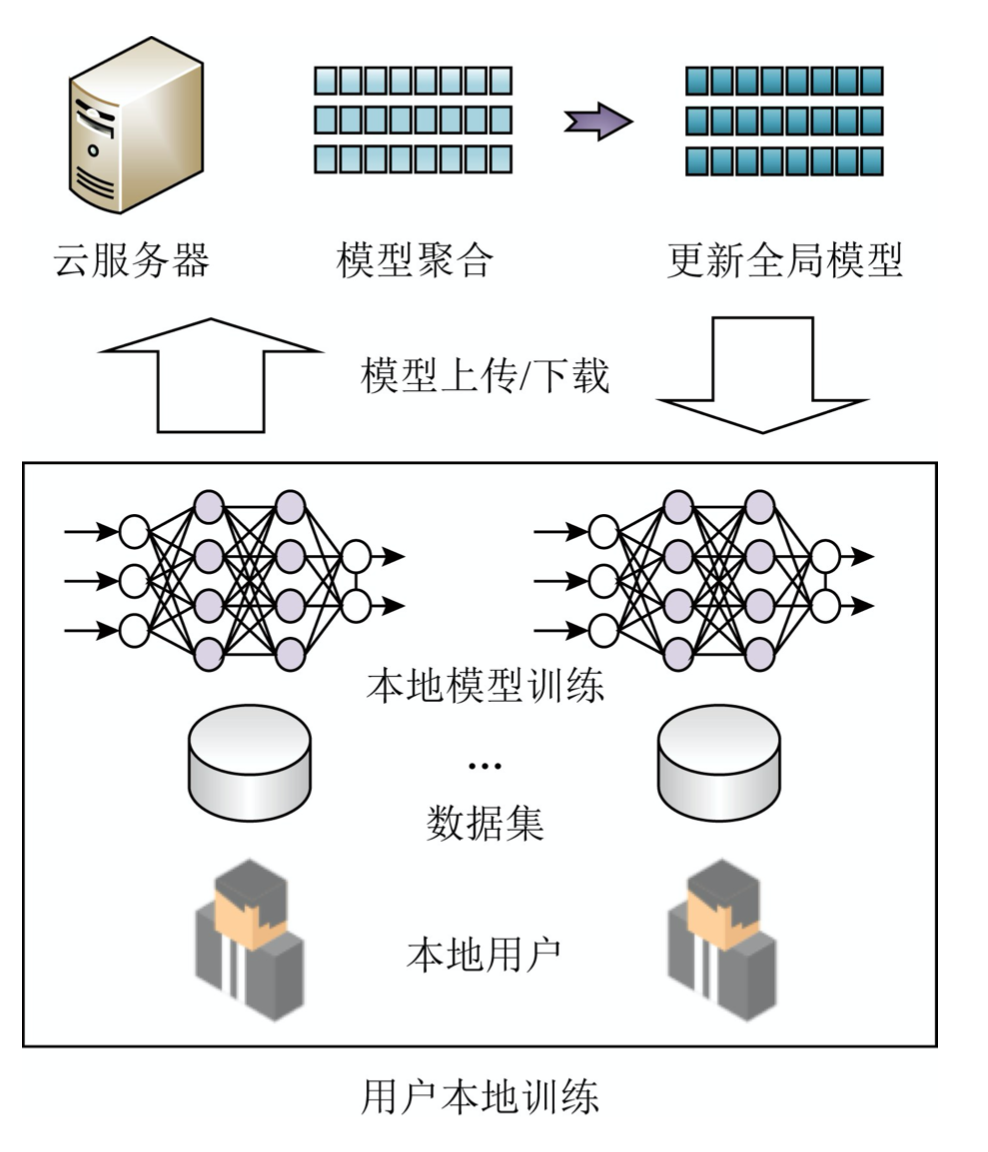
\includegraphics[scale=0.5]{fig2/C1/联邦学习训练模式}%联邦学习的系统架构
	\caption{联邦学习训练模型概览}
	\label{fig:联邦学习模型概况}	
\end{figure}

\section{安全性和隐私威胁}
尽管联邦学习解决了部分数据孤岛的问题,其本身还存在很多脆弱性和薄弱点。近年来,大量研究表明联邦学习机制仍然存在许多安全漏洞,这些漏洞可能被内部参与者和外部攻击者所利用,破坏联邦学习系统的安全性。由于联邦学习的框架并没有对参与方的资质进行校验、没有对模型的访问权加以约束,恶意的参与方可能将恶意的训练样本注入自己的本地模型中,影响全局模型的更新结果,导致最终的模型预测结果偏离,甚至全局模型不可用。此外,联邦学习也并没有考虑到对传递的参数进行保护,本地设备与中央服务器之间的通信信道有可能成为第三方窃取敏感信息的途径。本地设备上传到中央服务器的梯度本质是由模型和训练数据计算得到的函数,其中包含了关于本地训练数据的信息。攻击者可以从共享梯度中跟踪和获取参与者的隐私。综上,联邦学习的框架仍然存在本地训练数据泄漏、全局模型不可用等隐私问题。

图\ref{fig:联邦学习中的隐私威胁}大致概括了针对联邦学习隐私攻击的攻击者、攻击内容、攻击类型、攻击方式和攻击发生的时段。在联邦学习系统中,攻击方可能是内部攻击者,比如中央服务器、本地客户端。有一些恶意参与者作为本地客户端参与训练,修改本地的训练数据,注入一些有毒的数据,从而损害全局模型的准确性,操纵模型的预测结果;诚实但好奇的中央服务器通过观察本地客户端上传的梯度更新,篡改训练过程,并控制参与者对全局参数的视图。外部攻击者通过本地客户端与中央服务器之间的通信信道发起攻击,通过客户端上传的参数恶意的窃取用户的训练数据来生成样本原型。内部攻击通常比外部攻击更强,因为敌手拥有关于模型架构和内部参数的信息。

\begin{figure}[!hbt]
\centering
	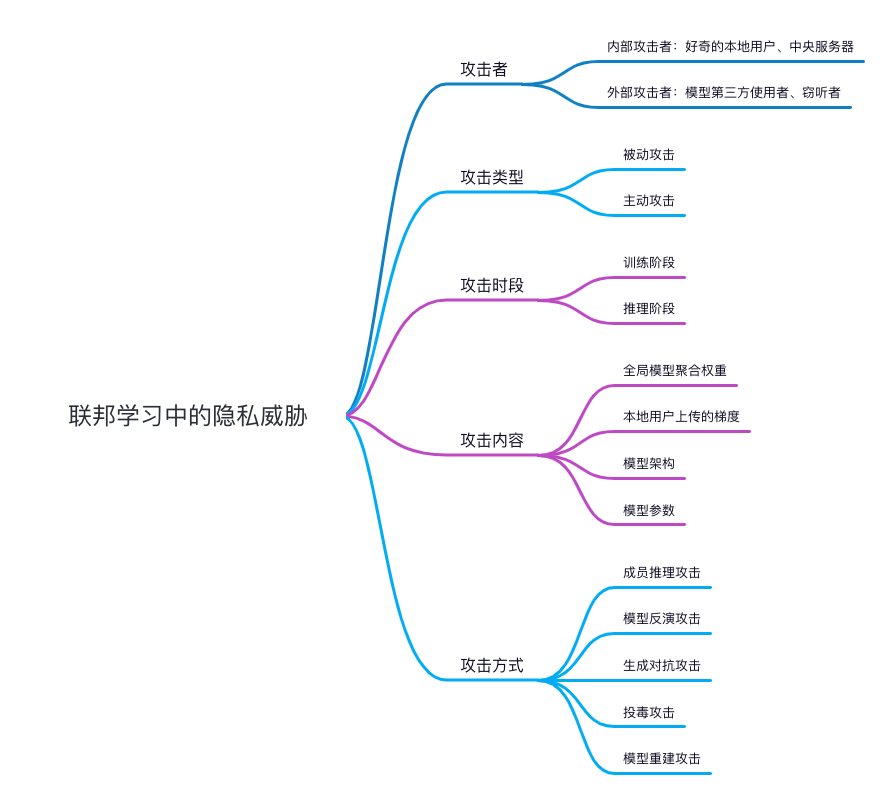
\includegraphics[scale=0.38]{fig2/C1/联邦学习中的隐私威胁}%联邦学习的系统架构
	\caption{针对联邦学习的隐私攻击}
	\label{fig:联邦学习中的隐私威胁}	
\end{figure}

针对联邦学习的攻击方式包括投毒攻击、模型反演攻击、成员推理攻击和生成对抗网络攻击等。

投毒攻击:投毒攻击通常发生在联邦学习的训练阶段。在联邦学习中,本地客户端在各自的设备上进行模型训练,将得到的训练参数上传给中央服务器。因为训练参数不需要通过可信机构的检查,所以有一些攻击者将恶意的训练样本注入自己的本地模型中,影响全局模型的更新结果,导致最终的模型预测结果错误甚至全局模型不可用。投毒攻击的影响对于许多企业和行业来说可能是致命的,在医疗部门、航空部门或道路安全方面甚至会危及生命。Marcus Comiter\upcite{ref56}曾使用投毒攻击进行实验,通过对熊猫的图像样本注入微小的恶意数据,导致算法预测结果发生重大变化,将熊猫识别为长臂猿。

模型反演攻击:当攻击者只能黑盒访问联邦模型时,攻击者仍然可以通过联邦学习系统提供的应用程序接口(Application programinterface,API)访问系统模型,通过向系统模型发送训练数据,获得所有表示类的预测标签和置信度信息,根据类标签和置信度数据重新建模,还原出目标模型的训练数据\upcite{ref11}。即使攻击者不清楚联邦模型的内部信息(训练参数、训练数据、模型结构等),依然可以通过API逆向反演获得所有预测数据的置信数据,由于置信信息代表了特征向量和标签类的关联性,攻击者将特征向量做为输入信息,对某一标签类进行分类或者回归得到置信度信息,其中置信度最高的类即为目标模型的目标类之一。

成员推理攻击:给定一个深度学习模型和一条数据样本(攻击者可以获取的知识范围),成员推理攻击旨在确定样本是否为用于构建此深度学习模型的训练集成员。例如,一个医疗机构根据基因型数据提供疾病预测的服务。假设保险公司持有某个客户A的基因型数据,通过对该疾病预测服务进行成员推理攻击,推断出A是否为某种疾病标签的成员样本,该公司就可以收取更多的费用以谋利。Shokri等人采用样本正确标签和目标模型预测的结果作为输入,通过影子学习的技术构建与目标模型的训练数据相近的数据集\upcite{ref13}。针对每一种数据样本,攻击者随机初始化一些数据记录作为影子模型的训练集数据。然后将此数据记录喂给目标模型得到预测向量,将所得的预测向量以及样本标签喂入攻击模型得到二分类的结果,达到推断任意样本是否在训练集中的目的。

生成对抗网络攻击:攻击者伪装成正常的用户参与联邦学习的训练,通过生成对抗网络(Generative Adversarial Networks,GAN)模型获得其他本地用户的训练数据。首先,攻击者在本地训练一个生成器网络和判别器网络,两者以零和博弈的思想进行对立训练,形成对抗生成式深度学习网络。生成器用来生成目标模型的伪样本,判别器被训练来区分图像是来自原始数据库还是由GAN生成的。攻击者将生成器生成的样本标记为"fake"类上传至全局模型,中央服务器通过聚合所有参与者上传的数据得到全局参数,攻击者通过基于假数据集的正常正向和反向计算获得假梯度,通过最小化假梯度和真实梯度之间的损失,反复优化假样本和标签,获得目标类的隐私数据。由于判别器参与了全局模型的训练,相当于在拥有该样本的用户训练数据上训练判别器,使得生成器有能力构造出与真实样本相似的伪样本。

\section{国内外研究现状}
随着针对联邦学习隐私攻击的模型增多,越来越多的研究者开始关注如何在联邦学习中应用隐私保护机制以防御上述的攻击模型。安全多方计算、同态加密和扰动技术是最常见的提高联邦学习中的安全性和隐私性的技术。

安全多方计算(Secure Multi-Party Computation,SMC)是由姚期智在1982年提出的\upcite{ref16},多个参与者在不泄露各自隐私数据情况下共同完成某项计算任务。安全多方计算是解决多方协同计算问题的一种解决方案,它必须保证计算中各方信息的保密性、独立性和准确性。当前,安全多方计算领域常见的技术主要包括混淆电路、零知识证明、不经意传输和秘密共享等。安全多方计算保护联邦学习的重点是如何在没有可信第三方的情况下安全地计算联邦学习中的经验风险最小化函数。同时,每个参与者都不可以获得任何关于其他用户的信息,除了梯度的聚合结果。Bonawitz等人利用SMC设计了一个联邦学习隐私保护框架,通过秘密分享技术安全地汇总用户的梯度,服务器只能看到聚合完成之后的梯度\upcite{ref3},不能知道每个用户的私有的真实梯度值,并且对用户的退出具有鲁棒性。然而,他们的模型由于涉及到学习过程中的多轮计算交互,在联邦学习通信回合数很大的情况下会导致通信性能大幅下降。

同态加密(Homomorphic Encryption,HE)是一种加密形式,允许第三方直接对密文进行算术运算\upcite{ref10}。在密文上进行计算后得到的结果进行解密,与明文上进行相同计算操作得到的结果是一致的。同态加密分为加法同态加密、乘法同态加密和全同态加密。同态加密保护联邦学习的隐私性主要通过将本地用户训练所得的梯度信息进行加密后上传至中央服务器,防止服务器对本地客户端上传的权重进行逆向工程从而反推出训练数据,确保每个客户端对全局模型的更改都保持隐藏状态。因为服务端接收的是本地客户端通过同态加密算法处理后的数据,这种模型的安全性是以服务器上的计算成本为代价的,加密场景的高计算复杂度会严重降低联邦学习的计算性能。 此外,由于需要传输公钥和秘钥也会增加额外的通信成本。Phong等人\upcite{ref23}提出了一个基于加法同态加密的联邦学习隐私保护方案,中央服务器可以根据同态操作,用加密的本地梯度更新全局模型参数。然而在基于联邦学习的系统中,有许多分布式设备(如智能手机和物联网设备)参与其中,用于解密的同一私钥需要分布到各个客户端,一旦持有相同秘钥的用户相互串通,将无法保证用户的数据隐私。

扰动技术的关键思想是在原始数据中加入噪声,使加躁后的数据与原始数据在统计特征上无法区分。三种广泛使用的扰动技术包括差分隐私、加法性扰动和乘法性扰动。差分隐私(Differential Privacy,DP)技术是基于概率统计模型来量化
数据集实例的隐私信息被披露的程度\upcite{ref75},其主要原理是向数据添加噪音,或使用概括方法来掩盖某些敏感属性\upcite{ref14},使至多相差1条数据的2个数据集的查询结果概率不可区分,以保护用户的隐私。差分隐私的优势在于其保护数据集所需要的隐私成本可以被量化,在通信效率和计算性能方面与明文计算相差不大。许多公司已经广泛采用差分隐私保护其联邦学习模型,包括谷歌、苹果、Uber、微软和LinkedIn。

在联邦学习框架应用差分隐私实现隐私保护基本可以分为两种方式:在本地模型训练阶段部署差分隐私;在全局参数聚合阶段部署差分隐私。

联邦学习中的本地用户进行模型训练的过程都可以看作是一次深度学习的过程。在深度学习中,差分隐私可以作为一种局部隐私保护方案来保护用户梯度的隐私。Song等人提出了一个$\left(\epsilon_{c}+\epsilon_{d}\right)$-差分隐私版本的随机梯度下降算法(DP-SGD),在本地模型的每一次迭代过程中对梯度添加高斯噪声,并通过差分隐私的组合性和隐私放大效果,得到完全隐私损失的上界\upcite{ref47}。然而,DP-SGD与SGD 相比严重降低了模型的准确率。当差分隐私提供的隐私保护强度增加时,在MNIST数据集上进行逻辑回归的训练和验证的损失率迅速增加。

Shokri等人\upcite{ref45}提出了一种选择性参数共享的差分隐私保护方案,通过对用户本地梯度绝对值进行排序,选择绝对值排名较大的梯度元素添加拉普拉斯噪声后参与联邦平均,然而随着模型迭代次数的增加,差分隐私的应用会导致模型的可用性下降。Choudhury等人\upcite{ref79}通过在联邦学习框架中应用分布式差分隐私机制,在两个真实的世界健康数据集上分析了不同的隐私预算对联邦模型性能的影响。他们给出的实验结果说明虽然差分隐私提供了一个强大的隐私水平,但是随着模型的通信回合数上升,整体隐私成本增加,模型性能大幅下降。

Geyer等人\upcite{ref48}研究发现与集中式学习相比,联邦学习中的梯度在整个训练过程中对噪声和批量大小具有不同的敏感度。他们的方案通过隐藏客户端的参与信息,实现客户层面的差分隐私,在分布式训练的过程中根据各个用户的隐私设置动态调整差分隐私的隐私参数,降低全局模型的性能损失。Truex等人\upcite{ref49}将差分隐私和同态加密技术相结合,在每个本地设备训练所得的权重上添加噪声后再使用同态加密技术进行加密,发送给中央服务器。中央服务器根据运算的同态性对加密后的数据进行聚合,更新全局参数。虽然通过差分隐私和同态加密加强了本地数据的隐私性,但是计算成本较高。

然而,Kang Wei等人\upcite{ref80}表示,Geyer\upcite{ref48}和Truex\upcite{ref49}的工作没有考虑到本地参数上传阶段的隐私保护,在向服务器上传训练结果时,客户的私人信息有可能被隐藏的敌手所截获。此外,这两篇文章缺乏对隐私性、收敛性能的具体分析。Kang Wei等人提出了提出了一个基于全局$(\epsilon, \delta)$-DP概念的新框架,对本地参数上传通道和全局参数下载通道定义不同的差分隐私要求,并在本地客户端和中央服务器采用不同的隐私参数添加高斯噪声。通过分析联邦学习模型损失函数的收敛界限,得出了以下结论:(1)模型的隐私保护水平越高,收敛性能越差;(2)在相同的隐私保护水平下,增加客户端的数量可以提高收敛性能;

总的来说,安全多方计算基于复杂的计算协议,同态加密的运算成本非常高,而现有的差分隐私保护联邦学习的方案很难在实现强隐私保护的同时,维持原有模型的精度。当使用较低的隐私预算达到较强的隐私保护的效果,可能使得模型难以收敛,可用性大幅下降;当隐私保护水平太低时,无法防御生成对抗网络攻击。当前的联邦学习中的隐私保护方案还有许多不足,很难在模型效用、数据隐私保护、通信性能这三个方面都达到满意的效果。

\section{研究内容与论文结构}
\subsection{研究内容}
联邦深度学习通过分布式的协作学习使得各个参与方在无需传递和共享本地的数据资源的情况下训练一个共同的、强大的深度学习模型。与传统的集中式深度学习相比,联邦学习在一定程度上缓解了数据孤岛和隐私泄露的问题。然而许多研究表明联邦学习机制仍然存在许多安全漏洞。联邦参与方、好奇的中央服务器以及外部的恶意敌手都有可能通过模型权重、共享的梯度和通信信道对联邦模型发起攻击,窃取用户的本地训练数据,破坏模型的可用性。差分隐私是当前保护联邦学习隐私安全的前沿技术,其通过严格的统计框架提供隐私保证和隐私成本计算,使得加躁后的梯度不能泄露关于实体数据的敏感信息。与安全多方计算和同态加密等密码学技术相比,差分隐私保护联邦学习的方案在通信性能和计算性能方面与明文计算相差不大。本文主要针对联邦学习的成员推理攻击和生成对抗网络攻击,设计基于差分隐私和安全混洗的隐私保护方案,对共享的梯度和模型权重进行隐私保护。本文的具体研究内容如下:

\begin{enumerate}
\item [(1)]在联邦学习的本地模型训练过程中,在每一轮随机梯度下降算法中对梯度注入高斯噪声,以防御成员推理攻击。现有的差分隐私保护深度学习方案大多数是基于固定的模型参数和隐私设置,很难在模型可用性和数据隐私性之间达到平衡效果。为了更好的解决现有的差分隐私保护数据隐私的同时,模型可用性下降的问题,本文对梯度加躁和梯度裁剪算法进行了以下优化:第一,根据逐层关联传播算法,在神经网络的前向和反向传播过程中分解神经元对于模型输出的贡献率,根据贡献率分配相应的隐私预算。保持整体的隐私预算不变,对于模型输出影响更大的梯度上添加较少的噪声,以减少梯度加躁对于模型可用性的影响。第二,在随机梯度下降算法的迭代过程中,根据之前训练所得梯度的统计特征,动态调整梯度裁剪阈值,尽可能的保留梯度中的有效信息。第三,本文采用“Moments Accountant”机制分析加噪累积产生的隐私预算,使得隐私损失的计算更加精确。

\item [(2)]当联邦学习中的用户数量达到千万量级时,在本地设备的模型训练上采用差分隐私技术,对于聚合后的梯度平均估计误差能达到$O\left(\frac{\sqrt{d \log d}}{\epsilon \sqrt{m}}\right)$。如果在迭代训练过程中的每一次迭代都应用本地差分隐私,隐私损耗就会成倍累积,从而导致聚合参数上的噪声溢出,影响全局模型的发布结果,增加了通信成本。为了解决这一问题,本文对基于本地差分隐私的联邦学习隐私保护方案进行了以下优化:第一,基于指数机制的打分函数和稀疏向量的思想对梯度进行采样扰动,相比本地差分隐私而言降低了计算复杂度;第二,在联邦学习中动态的调整客户端采样率,使用指数衰减率来递减训练过程中的采样率,在相同的通信回合下降低整体的通信成本;第三,在中央服务器和本地设备之间引入混洗器。混洗器将所有客户上传的加密数据集合中的向量元素进行拆分和随机置换,得到一个无序的消息集合。混洗和采样的操作达到了双重的隐私放大效应,从 $\left(\epsilon_{c}+\epsilon_{l}\right)$的本地差分隐私放大至 $\bar{\epsilon} $-中央差分隐私。在本地设备添加更少的噪声,而在中央服务器上达到相同的隐私保护效果,兼顾隐私保护能力与模型可用性。

\end{enumerate}

\subsection{论文结构}
本文一共五个章节,主要内容的组织安排如图所示:

第一章介绍了联邦学习的研究背景和存在的隐私威胁,并具体阐述了针对联邦学习的差分隐私保护的研究现状与发展方向,最后介绍了本文的相关工作和贡献。

第二章详细介绍了关于本文研究内容的基础知识,包括联邦学习的工作流程,差分隐私的基本概念和定理、神经网络的基本结构和训练算法。

第三章是基于本地自适应差分隐私保护联邦学习的共享梯度。首先,在引言部分介绍了差分隐私保护深度学习算法的四种扰动方式,主要针对梯度扰动分析了前人方案的不足之处,接着提出了本文所设计方案的两个创新点,依次详细的描述了梯度的自适应加躁算法和梯度的自适应裁剪算法的设计思路和实现流程。将梯度自适应的加躁和裁剪算法应用在随机梯度下降算法中,得到本地模型训练的核心算法,并结合MA机制分析总隐私损失。最后,我们通过三方面的实验对本地自适应差分隐私保护方案进行了全面的评估:其一,分析噪声水平、裁剪阈值、隐藏层数量这些参数对模型分类准确率影响;其二,与非隐私的SGD、前人提出的差分隐私SGD方案,比较各个方案在相同隐私预算的情况下模型分类所能达到的准确率和模型收敛速度;其三,针对部署了本地自适应差分隐私的联邦学习模型训练成员推理攻击模型,评估隐私保护效用。

第四章针对高维聚合场景下噪声成倍累积的问题,设计了Top-K梯度安全混洗算法。首先,定义了威胁模型和隐私表述,描绘了基于安全混洗的联邦学习模型框架,依次详细的描述了本地top-K梯度采样算法、客户端动态采样算法和梯度混洗算法的设计思路和实现流程。接着,证明了采样和混洗算法实现了$\left(\epsilon_{c}+\epsilon_{l}\right)$-本地差分隐私到 $\bar{\epsilon} $-中央差分隐私的隐私放大效用。最后,我们通过三方面的实验对Top-K梯度安全混洗算法进行了全面的评估:其一,分析客户端数量$N$、梯度选择的比率、客户端采样比$f_{r}$和最大聚合次数对于模型分类准确率的影响;其二,与非隐私的SGD、前人提出的差分隐私SGD方案进行对比实验,评估指标为模型分类准确率和通信性能;其三,针对部署了Top-K梯度安全混洗算法的联邦学习模型训练生成对抗网络攻击模型,评估隐私保护效用。

第五章是对文本的工作内容的总结和未来研究方向的展望。首先对本文的研究内容进行了概括,并总结了现有方案的不足之处,之后对未来的研究和改进方向进行了展望。

\section{本章小结}
这一章节为绪论,首先介绍了联邦学习的研究背景和存在的隐私威胁,并具体阐述了针对联邦学习的差分隐私保护的研究现状与发展方向,最后介绍了本文的相关工作、贡献和论文的组织结构。


\chapter{基础知识}
\label{ch2}
在本章节中我们将介绍本文研究所需要的一些基本知识,有助于更好的理解之后章节的内容。

\section{神经网络}
\subsection{基本结构}
深度学习算法的输入数据通常表示为一组样本。每个样本将包含一组特征值。例如,考虑一张 100x100 像素的照片,其中每个像素由一个数字(0-255灰度)表示。我们可以用这些像素值组成一个长度为 10,000 的向量,通常称为特征向量。每张照片,表示为一个特征向量,可以与一个标签(例如,照片中人物的名字)相关联。深度学习算法将使用由多个特征向量及其相关标签组成的训练集来构建深度学习模型,这个过程称为模型的训练。当给出一个新的测试样本时,深度学习模型应该给出预测的标签。模型准确预测标签的能力是衡量该模型对未知的数据的泛化程度的标准,是通过测试误差(泛化误差)衡量的。模型的泛化能力取决于训练数据的质量和数量、使用什么深度学习算法来构建模型、深度学习算法超参数的选择(例如使用交叉验证),甚至是特征的提取方法。

深度学习模型通常采用神经网络的形式。已经为不同的应用提出了各种神经网络架构,例如多层感知器、卷积神经网络和循环神经网络。神经网络\upcite{ref34}最初的设计灵感来源于人脑的结构。众所周知,人类的大脑是处理信息的重要部分。人脑中含有大量的神经元,当人脑接受到外部环境的刺激时,信号随着神经元一层一层的传入人脑神经中枢,神经中枢根据接受到的信号给出判断,然后再随着输出神经网络传递,最终作出不同的行为或者判断。神经网络就是模拟人脑处理信息的流程对数据进行学习的。

神经网络的基本组成单元是神经元,一个神经网络可能包含数百亿个简单的神经元,它们按层排列,密集而复杂的相互连接着。神经网络中每一层有多个神经元,层与层之间是“前馈传播”的,也就是说,网络中的数据只在一个方向上移动。第l层的神经元与第l-1层的所有神经元相连,从这些神经元接收数据,这就是全连接的概念。每一层的神经元只有可能与其前一层和后一层的神经元相连接,不存在跨层连接。

\begin{figure}[!hbt]
\centering
	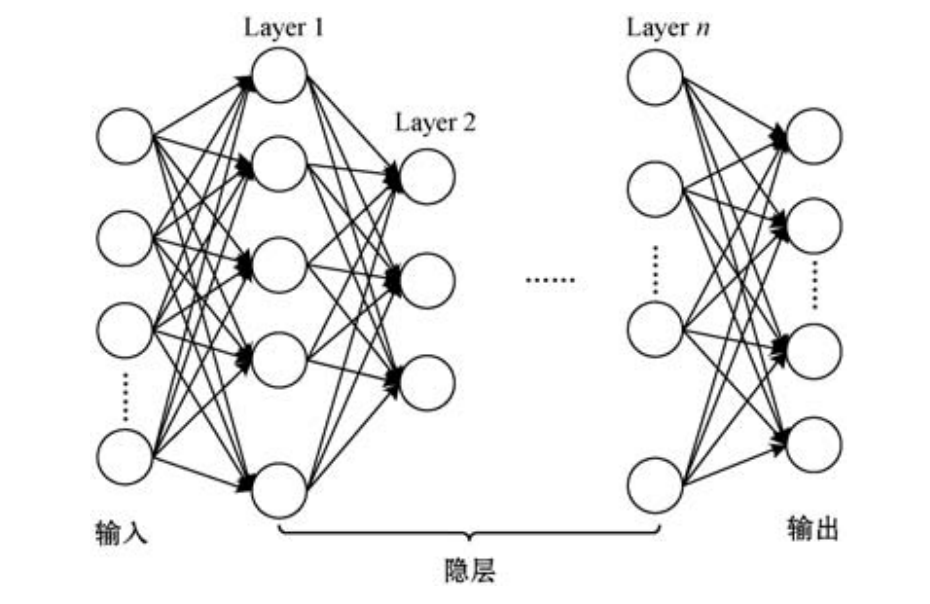
\includegraphics[scale=0.5]{fig2/C2/深度神经网络结构图}%联邦学习的系统架构
	\caption{神经网络结构图}
	\label{fig:神经网络结构图}	
\end{figure}

如图\ref{fig:神经网络结构图}所示,一个神经网络由一个输入层、一个输出层以及输入和输出之间的一系列隐藏层组成。每一层都是一组称为神经元的单元,它们连接到上一层和下一层的其他神经元。输入层用于接收信息,当一个神经网络被训练时,其所有的权重和阈值最初都被设置为随机值,然后训练数据被送入输入层;之后传入隐藏层进行特征的提取、网络权重的调整,使得隐藏层的神经单元对某种模式形成特定的反应;最后传导到输出层,输出模型判断的结果。神经元之间的每个连接都可以通过应用线性函数和元素级非线性激活函数(例如 sigmoid 或 ReLU)将信号传输到下一层的另一个神经元。通过类似于人脑处理信息的方式,神经网络在重复训练的过程中调整网络权重,使最终输出的预测结果与真实结果更加接近,但是如何调整网络权重使误差最小呢?

反向传播和随机梯度下降是训练深度学习模型和寻找最佳参数的常用方法。在深度神经网络中,对每个训练样本,通过前向传播算法从输入层、隐藏层到输出层依次训练,在输出层得到预测的结果,然后根据损失函数(如交叉熵损失函数、均方误差损失函数等)计算预测值与真实值之间的差异程度,之后根据反向传播算法调整权重系数,更新网络参数,使得损失函数的值最小,模型达到全局最优。

\subsection{随机梯度下降算法}
随机梯度下降算法(Stochastic Gradient Descent,SGD)是一种主流的用于机器学习和深度学习模型优化的迭代方法,从数据集中随机采样一批训练岩本,迭代运行梯度下降算法,使损失函数收敛到局部最小值,以找到使模型达到全局最优的权重系数,具体的算法如所示。

\begin{algorithm}[!htb]
	\caption{随机梯度下降算法}
	\label{随机梯度下降算法}
	\begin{algorithmic}[1]
		\footnotesize
		\STATE \textbf{输入:} 学习率$\alpha$
		\STATE \textbf{输出:} 初始参数$\theta$
		\STATE 初始化模型权重$\theta$,作为梯度下降的起始点
		\WHILE{模型未达到全局最优点}
		\STATE 从训练集中均匀抽出一小批量(minibatch)样本:$\mathbb{B}=\left\{x^{(1)}, \ldots, x^{\left(m^{\prime}\right)}\right\}$
		\STATE 计算梯度估计:$$
g=\frac{1}{m^{\prime}} \nabla_{\theta} \sum_{i=1}^{m^{\prime}} L\left(x^{(i)}, y^{(i)}, \theta\right)
$$
		\STATE 梯度下降:$$
\theta=\theta-\epsilon g
$$
		\ENDWHILE
	\end{algorithmic}
\end{algorithm}

\subsection{经验风险最小化}
在神经网络中,模型通过不断的学习数据集中的特征得到预测值,通过损失函数计算预测值与真实值之间的误差,之后再采用反向传播算法调整权重系数使得最终的损失函数的值最小。整个模型训练的过程可以理解为经验风险最小化(Empirical risk minimization,ERM)问题:
\begin{equation}\label{eq:ERM}
F(\boldsymbol{\theta}):=\frac{1}{n} \sum_{i=1}^{n} f_{i}(\boldsymbol{\theta})
\end{equation}

模型在训练集$S=$ $\left\{\left(\mathbf{x}_{1}, y_{1}\right), \ldots,\left(\mathbf{x}_{n}, y_{n}\right)\right\}$上进行训练,其中,$F(\boldsymbol{\theta})$表示经验损失函数;$f_{i}(\boldsymbol{\theta})=\ell\left(\boldsymbol{\theta} ; \mathbf{x}_{i}, y_{i}\right)$表示在第$i$个训练样本$\left(\mathbf{x}_{i}, y_{i}\right)$上定义的损失函数;$\boldsymbol{\theta} \in \mathbb{R}^{d}$表示模型最终训练得到的权重参数。模型的训练目标是找到最终的权重参数$\widehat{\boldsymbol{\theta}} \in \mathbb{R}^{d}$ ,使得公式\ref{eq:ERM}所计算得到的经验风险值最小。

\section{联邦学习}
传统的集中式深度学习需要将训练数据放在一起到数据中心。该模型以集中方式进行训练。而联邦学习允许数据所有者拥有一个私人学习网络,该网络使用本地数据集进行训练。之后,每个参与者将本地模型的梯度上传到云服务器。通过使用云服务器收集的全局梯度进行更新,可以避免局部模型过度拟合。此外,它还保护本地数据不被其他参与者或云服务器直接知道。联邦学习的基本工作流程如下:
\begin{itemize}
\item \textbf{初始化:}
所有用户在个字的设备上都有一个预先分配的神经网络模型,并且可以自愿加入联邦学习协议,指定相同的深度学习和模型训练目标。
\item  \textbf{本地训练:}在一个给定的通信回合中,联邦学习参与者首先从中央服务器下载全局模型参数,然后在各自的本地数据集$D_{i}$上进行模型训练,更新模型参数:$\omega_{i}^{r+1} \leftarrow \omega_{i}^{r}-\eta_{i} \nabla g\left(D_{i}^{t}, \omega_{i}^{r}\right)$
\item \textbf{中央参数聚合:}中央服务器等待所有本地客户端将更新后的模型参数$M1,M2....M_{n}$上传,聚合得到全局模型的参数,之后更新全局模型:$\omega^{r+1} \leftarrow \omega^{r}-\eta \frac{\sum_{U_{i} \in U^{t}} \varsigma U_{i}}{\sum_{U_{i} \in U^{t}}\left|D_{i}^{t}\right|}$
\item \textbf{迭代更新:}迭代地执行上述步骤直至全局模型参数满足收敛条件,最终得到最优的全局模型。
\end{itemize}

\begin{figure}[!hbt]
\centering
	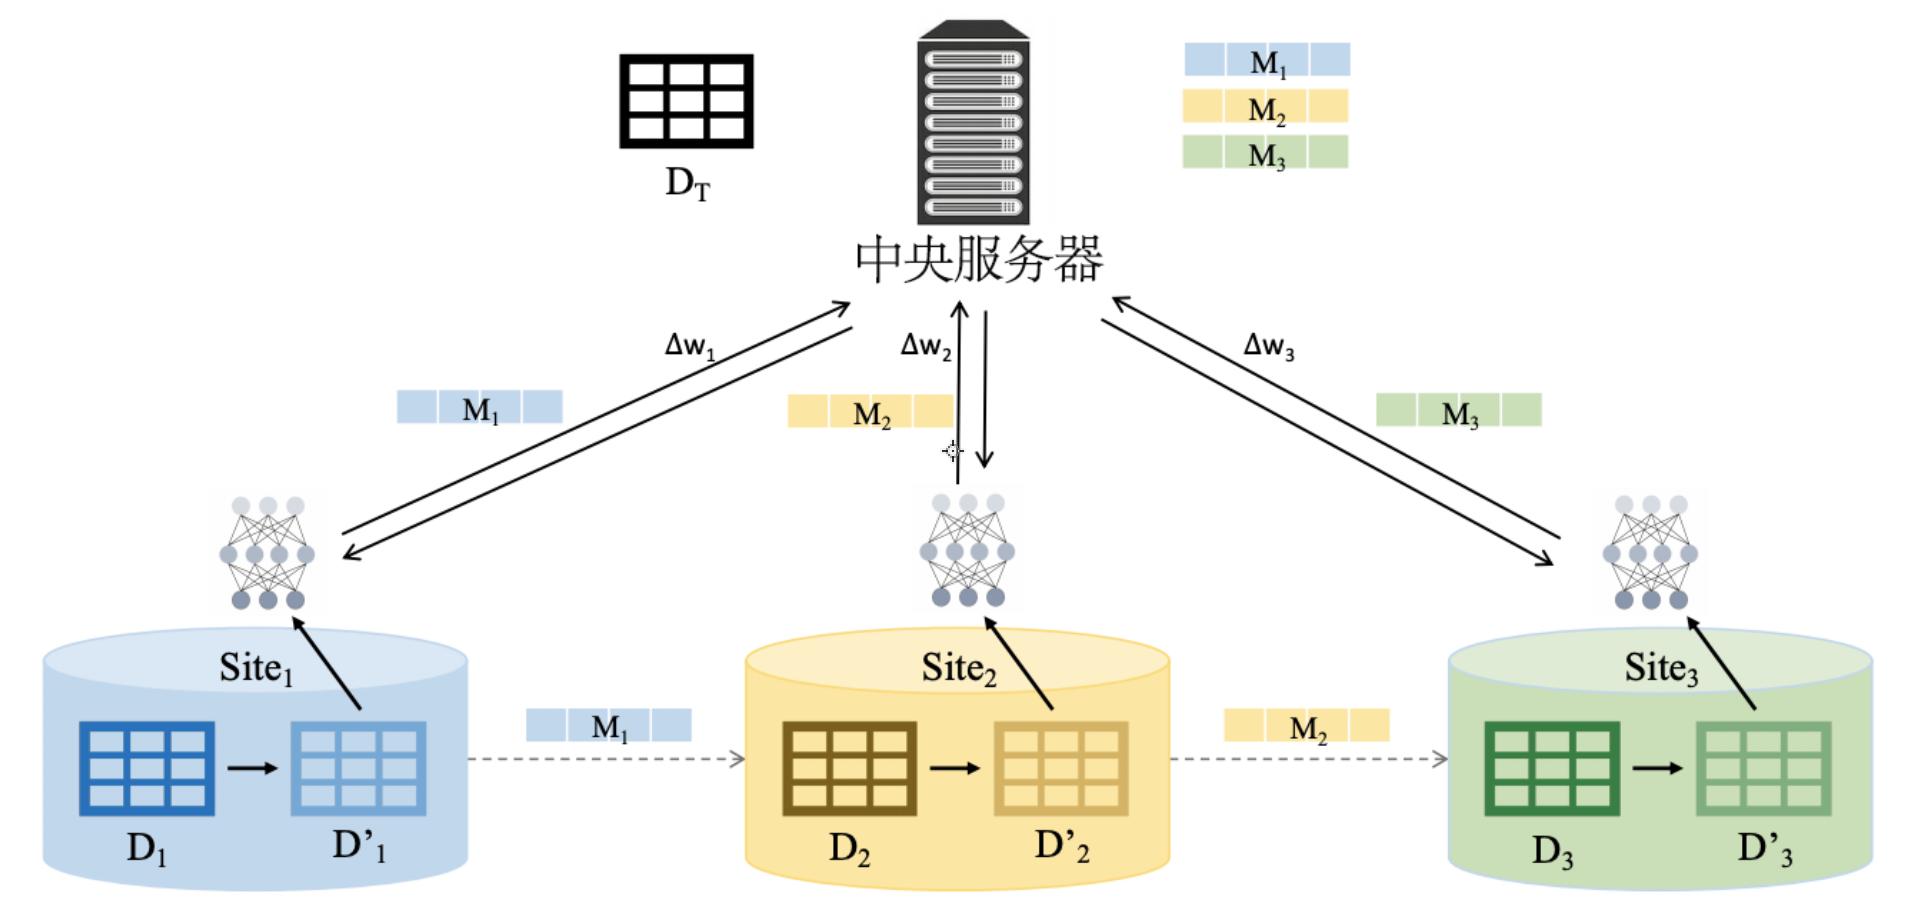
\includegraphics[scale=0.45]{fig2/C2/联邦学习模型流程}%联邦学习的系统架构
	\caption{联邦学习模型工作流程}
	\label{fig:联邦学习模型工作流程}	
\end{figure}

\section{差分隐私}
\subsection{基本定义}
\begin{define}[邻近数据集]\label{邻近数据集}
现有两个属性相近的数据集$D$和$D^{\prime}$,他们的数据记录差为$D \Delta D^{\prime}$,如果$\left|D \Delta D^{\prime}\right|=1$,则称数据集$D$和$D^{\prime}$为邻近数据集(Adjacent Dataset)。
\end{define}

\begin{figure}[!hbt]
\centering
	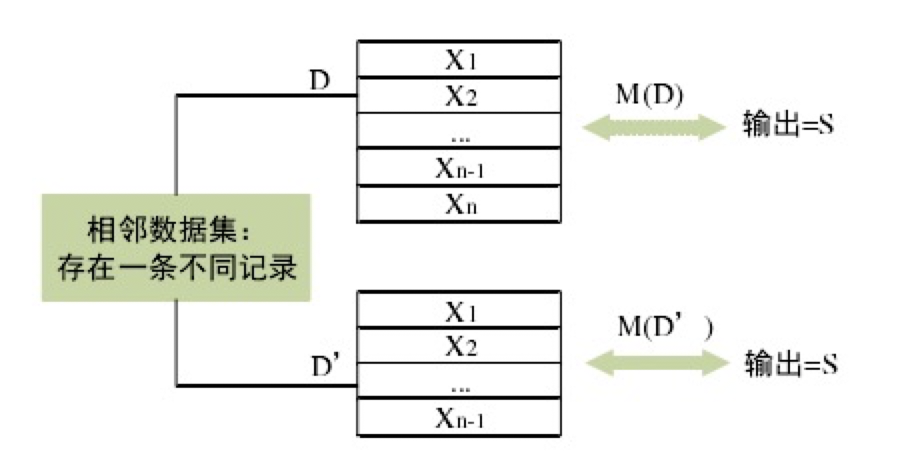
\includegraphics[scale=0.6]{fig2/C2/相邻数据集示意图}%联邦学习的系统架构
	\caption{差分隐私的相邻数据集示意图}
	\label{fig:相邻数据集示意图}	
\end{figure}

2016年,Dwork\upcite{ref14}等人首次提出了差分隐私的概念,它在针对数据隐私泄漏的新型隐私定义,目的是使数据库的查询函数对数据集中单条记录的变化不敏感。其思想是添加一定量的噪音来随机化给定算法的输出,从而使攻击者无法区分任何两个相邻的输入数据集的输出。具体的定义如下:
\begin{define}[(ε,δ)-差分隐私]\label{(ε,δ)-差分隐私}
$\mathcal{D}$表示数据集合,$D$和$D^{\prime}$ 为邻近数据集。现有随机算法$M: D \rightarrow R$,D表示定义域,R表示值域。如果对于任意两个邻近数据集$S, S^{\prime} \in \mathcal{S}^{n}$和输出子集$O \subseteq \mathcal{R}$时,总有$$
\operatorname{Pr}[\mathcal{M}(D) \in S] \leq e^{\epsilon} \operatorname{Pr}\left[\mathcal{M}\left(D^{\prime}\right) \in S\right]+\delta
$$,则称该随机算法满足 $(\varepsilon, \delta)$-差分隐私。
\end{define}
添加项$\delta \in[0,1]$表示以某种概率打破$(\epsilon, 0)$-差分隐私。当$\delta=0$时,则将$M$称为$\epsilon$-差分隐私。$\epsilon$和$\delta$表示隐私预算参数,$\epsilon$和$\delta$越小,算法能提供的隐私保证程度越强。

差分隐私保护的实现是在查询函数的返回值中注入一定量的干扰噪声,但是注入的噪声量太大会影响最终结果的准确性,太少则无法保障数据的隐私性。那么如何衡量添加的噪声量,既能保障数据的安全,又能维持数据的可用性呢?这里针对数据集提出敏感度的概念,对于相邻数据集$D$和$D^{\prime}$,某个查询函数在此相邻数据集上所输出的结果的不同程度代表了此函数的敏感度,而函数的敏感度决定了需要在函数中添加的噪声量来实现最终输出结果的差分隐私,因此加入的噪声量与函数的敏感度高度相关的。

\begin{define}[函数敏感度]\label{函数敏感度}
假设存在查询函数 $f: D \rightarrow R^{d}$, 输入为一数据集,输出为$d$维的实数向量。 对于任意的邻近数据集 $D$ 和 $D^{\prime}$,函数$f$的$L_{1}$敏感度($L_{2}$敏感度)表示为$\Delta_{1}(q)$($\Delta_{2}(q)$),计算公式如下:
$$
\Delta_{1}(q)=\max _{D \sim D^{\prime}}\left\|f(D)-f\left(D^{\prime}\right)\right\|_{1}, \quad \Delta_{2}(q)=\max _{D \sim D^{\prime}}\left\|f(D)-f\left(D^{\prime}\right)\right\|_{2}
$$
称为函数 $f$ 的全局敏感度。
\end{define}

\subsection{实现机制}
在差分隐私的实际应用中,如何针对不同的场景和问题设计添加噪声的机制使算法能满足差分隐私保护的要求呢?差分隐私的实现机制主要分为拉普拉斯机制(Lapalace Mechanism)\upcite{ref9}、指数机制(Exponential Mechanism)\upcite{ref32}与高斯机制(Gaussian Mechanism)\upcite{ref33}。其中,指数机制适用于非数值型结果的隐私保护,拉普拉斯机制和高斯机制适用于对数值型结果的隐私保护\upcite{ref35}。

\begin{theorem}[拉普拉斯机制]\label{拉普拉斯机制}
给定一个基于数据集$D$的查询函数$f(D)$,算法$\ddot{f}(D)$满足 $\varepsilon$-差分隐私, 当:
$$
\ddot{f}(D)=f(D)+\operatorname{Lap}\left(\frac{G S}{\epsilon}\right)
$$
\end{theorem}
其中,噪声参数满足$\operatorname{Lap}\left(\frac{G S}{\epsilon}\right)$的 Laplace 分布,$GS$表示数据集的敏感度。

与拉普拉斯机制类似,高斯机制通过对数据中的所有维度添加满足高斯分布的噪声实现差分隐私。
\begin{theorem}[高斯机制]\label{高斯机制}
一个查询函数 $f: D \rightarrow R$, 该算法的敏感度表示为$S_{f}$,算法$M$ 满足 $\varepsilon$-差分隐私,当:
$$
\mathcal{M}(d) \triangleq f(d)+\mathcal{N}\left(0, S_{f}^{2} \cdot \sigma^{2}\right)
$$
\end{theorem}
其中,$\mathcal{N}\left(0, S_{f}^{2} \cdot \sigma^{2}\right)$是满足正态(高斯)分布的,均值为0,标准差为 $S_{f} \sigma$。当$\epsilon \in(0,1]$,$\sigma \geq$ $\sqrt{2 \ln (1.25 / \delta)} \Delta_{A} / \epsilon$,算法$M$ 满足 $(\epsilon, \delta)$-差分隐私。其中$\epsilon$代表了隐私保护的程度,与噪声量呈负相关;$\delta)$是松弛项,表示允许以多少的概率打破差分隐私。

但是对于离散型的查询结果或数据要如何处理呢?这就产生了指数机制,通常使用指数机制来随机选择离散的输出结果来满足差分隐私。指数机制整体的思想就是,对于一个查询函数,不是确定性的输出一个$R_{i}$结果,而是以一定的概率值返回结果,从而实现差分隐私。

\begin{theorem}[指数机制]\label{指数机制}
指数机制满足差分隐私, 如果:
$$
A(D,u)=\left\{p: \mid \operatorname{Pr}[p \in O] \propto \exp \left(\frac{\varepsilon u(D,p)}{2 \Delta u}\right)\right\}
$$
\end{theorem}
其中 $u(D,p)$为评分函数,评分越高,则输出的概率越大\upcite{ref53},$\Delta u$表示$u(D,p)$的全局敏感度。

\subsection{相关定理}

在解决一个复杂的差分隐私保护问题时,可能在多个场景,多个步骤多次应用差分隐私技术,在这种情况下,如何保证最终结果的差分隐私性,以及隐私保护的程度该如何去度量呢?这里引出差分隐私的三个最重要的性质:组合性、可量化性和后处理不变性\upcite{ref35}。
组合性指的是将多个差分隐私的算法进行串行组合或者并行组合后得到的算法整体依然满足差分隐私。

\begin{theorem}\label{串行组合}
对于任意满足$(\varepsilon, \delta)$-差分隐私的算法$\mathcal{M}_{1}$和$\mathcal{M}_{2}$,算法 $\mathcal{M}_{3}$:$\mathcal{M}_{3}(\vec{x})=\left(\mathcal{M}_{1}(\vec{x}), \mathcal{M}_{2}(\vec{x})\right)$也满足$(\varepsilon, \delta)$-差分隐私。
\end{theorem}

\begin{theorem}\label{并行组合}
对于任意满足$(\varepsilon, \delta)$-差分隐私的算法$\mathcal{M}_{1}, \ldots, \mathcal{M}_{d}$,算法 $\overline{\mathcal{M}}$:$\overline{\mathcal{M}}(\vec{x})=\left(\mathcal{M}_{1}(\vec{x}), \ldots, \mathcal{M}_{k}(\vec{x})\right)$ 也满足$\left(\varepsilon \cdot\left(\sqrt{2 d \ln (1 / \delta)}+\left(e^{\varepsilon}-1\right) \cdot d\right), \delta \cdot(d+1)\right)$-差分隐私。
\end{theorem}

通过差分隐私的串并行组合定理,人们可以利用基础的差分隐私算法设计出复杂的满足差分隐私的系统,只要算法中的每一个步骤都满足差分隐私要求,那么这个算法的最终结果将满足差分隐私特性,这也是差分隐私的重要优势之一。 

可量化性指的是在算法中添加随机扰动以满足差分隐私时,可以精准的计算所添加的噪声量,代表了整体算法满足差分隐私所需要的隐私预算,这里的隐私预算是可量化的。后处理一致性则是指在对满足差分隐私的算法进行进一步处理时,只要不引入额外的信息,其输出依然满足差分隐私,整体的隐私保护力度也是不变的。在差分隐私的应用程序中,通常结合串并行组合定理分析算法累积的总体隐私预算和隐私成本。

对于一个随机算法设计满足差分隐私的方案通常包括以下步骤:
\begin{enumerate}
\item [(1)] 将敏感度有界的函数相组合使得整个系统的查询函数敏感度有界
\item [(2)] 选择合适的噪声机制和参数实现差分隐私
\item [(3)] 结合串并行组合定理分析算法累积的总体隐私预算和隐私成本
\end{enumerate}

\section{联邦学习中的差分隐私}
现有的在联邦学习模型中应用差分隐私实现隐私保护主要有两种机制:中央差分隐私和本地差分隐私。在中央差分隐私机制中,它要求一个可信的第三方服务器对所有用户的数据分析结果进行隐私化处理。在联邦学习的场景中,实现中央差分隐私需要一个可信的第三方服务器,如果中央服务器是可信的,通过定义全局函数的敏感度,在查询结果上添加噪声,使得全局聚合函数的输出结果是不可区分的;如果中央服务器是诚实但好奇的,在本地客户端和中央服务器的通信信道中间新增一个可信第三方服务器对所有用户的训练结果添加拉普拉斯扰动实现差分隐私。与中央差分隐私机制不同,本地差分隐私机制没有对第三方服务器的任何假设,所有用户的训练结果在本地设备对数据添加随机扰动后上传至中央服务器,它可以为每个用户提供强大的隐私保证。然而,由于每个本地用户都必须在自己的数据中添加高斯噪声,所以模型总体的噪声相比中央差分隐私要大得多,导致统计结果可用性差。

在联邦学习环境中,用户面对的可能是大量的非可信实体,而一个真正可信的数据机构又很难找到。本文主要应用本地差分隐私机制实现联邦学习的隐私保护,同时引入其他技术使整体的噪声量降低,降低全局模型的准确率损失。接下来介绍在联邦学习中应用本地差分隐私的基本流程:
\begin{itemize}
\item \textbf{本地计算:}
客户端 $\mathrm{i}$ 根据本地数据库 $\mathcal{D}_{\mathrm{i}}$ 和接受的服务器的全局模型 $\mathrm{w}_{\mathrm{G}}^{\mathrm{t}}$ 作为本地的参数,即 $\mathrm{w}_{\mathrm{i}}^{\mathrm{t}}=\mathrm{w}_{\mathrm{G}}^{\mathrm{t}}$, 采用梯度下降策略进行本地模型训练得到 $\mathrm{w}_{\mathrm{i}}^{\mathrm{t}+1} \quad(\mathrm{t}$ 表示当前通信回合) 。

\item \textbf{模型扰动:}
每个客户端产生一个随机噪音 $\mathrm{n},\mathrm{n}$ 是符合高斯分布的,使用 $\overline{\mathbf{w}_{\mathrm{i}}}^{\mathrm{t}+1}=\mathrm{w}_{\mathrm{i}}^{\mathrm{t}+1}+\mathrm{n}$ 扰动本地模型 (这里注意w是一个矩阵,n表示对矩阵的每一个元素添加噪音)。

\item \textbf{模型聚合:}
服务器使用参数聚合算法聚合从客户端收到的 $\overline{\mathrm{w}}_{\mathrm{i}} \mathrm{t}+1$ ,得到新的全局模型参数 $\mathrm{w}_{\mathrm{G}}^{\mathrm{t}+1}$, 也就是扰动过的模型参数。

\item \textbf{模型广播:}
服务器将新的模型参数广播给每个客户端。

\item \textbf{全局收敛:}
重复步骤(1)-(4)直至全局模型收敛。
\end{itemize}

\section{本章小结}
本章节介绍了论文研究内容所需了解的基础知识,包括差分隐私、神经网络和联邦学习。本节还介绍了联邦学习的基本工作流程,本文所提出的隐私保护方案都是针对联邦学习中的隐私泄露问题。此外,本节介绍了神经网络中前向传播和反向传播的算法以及具体实现方法——随机梯度下降算法,第三章所提出的本地自适应梯度加躁方案就是基于神经网络的结构进行设计;差分隐私是本文所重点关注的实现隐私保护的机制,论文重点讲解了差分隐私的定义、实现机制和相关定理。最后,论文介绍了传统的在联邦学习中实现差分隐私的方式,包括本地差分隐私和中央差分隐私。
\chapter{联邦学习中的自适应本地差分机制}

\label{ch3}
与传统的集中式深度学习相比,联邦学习通过分布式训练在一定程度上缓解了隐私泄漏的问题。然而,许多研究表明,攻击者仍然可以通过模型训练的梯度损害用户的隐私[13]。文献[20]表明,深度学习技术可以"记忆"模型中的训练数据信息。在这种情况下,敌方一旦通过白盒推理攻击或者黑盒推理攻击访问模型,就可以推演出客户端本地的训练数据。

在传统的集中式隐私保护方案中,数据管理者倾向于给每个用户的数据以相同的隐私预算。同样的隐私预算忽略了用户之间的差异。有些用户希望有更好的隐私保护。而有些用户对某些数据的隐私不敏感。在这种情况下,由于联邦学习模型是分布式结构,从一个大数据库到许多小数据库,所以对于每个用户来说。他们只需要关心他们自己的隐私。他们可以设置不同的隐私预算方案,而不是传统的统一分配,然后在最坏的的情况下注入噪音。所以我们需要注入更少的整体噪音。

机器学习中模型的优化问题可以概括为ERM(经验风险最小化)问题:
\begin{equation}\label{eq:ERM}
\arg \min _{\theta \in \mathcal{C}}\left(F(\theta):=\frac{1}{m} \sum_{i=1}^{m} F_{i}(\theta)\right)
\end{equation}

从隐私保护的角度讲,我们只要截断了从原始输入到输出,在其中加入一道隐私保护屏障,具体在哪一步截断则对应于不同的方法。差分隐私保护机器学习的方法具体有以下几种:
\begin{itemize}
	\item \textbf{输入扰动:} 输入扰动是在获取的训练数据上直接添加噪声,之后的模型训练和优化都是基于加躁后的训练数据。
	\item \textbf{输出扰动:} 输出扰动沿袭了拉普拉斯机制最简单的思路,即考虑函数输出的敏感度来添加噪声,那么在ERM公式中我们只需要考虑argmin函数输出的敏感度,基于这个敏感度来添加拉普拉斯噪声即可得到一个简单的满足差分隐私的ERM方法。
	\item \textbf{梯度扰动:} 梯度扰动是在执行最小化损失函数的过程中,设计满足差分隐私的算法。
	\item \textbf{目标扰动:} 目标扰动是在模型的目标函数中添加一个随机量,以使得最终模型的输出满足随机性。
\end{itemize}

基于输入的扰动和输出的扰动基本可以视为一个黑匣子模型,简单直接。但是这种添加噪声的方式无法对训练过程中数据的相互依赖性和输出有效性作出有用的、紧密的描述。在输入数据中加入过多的噪声,可能会影响模型训练的收敛性。在输出参数中加入过于保守的噪声,也就是根据最坏的攻击情况去添加噪声,可能会影响模型的实用性。因此本文采用一种更加复杂的方法来分析训练过程中训练数据对模型输出的贡献比率,然后根据每一层神经网络对模型输出的贡献率,在梯度上自适应添加噪声。

基于梯度加噪的差分隐私保护方法作为主流的差分隐私应用于深度学习模型的方法之一,方案的目标是满足差分隐私条件下实现最优的模型可用性。文献[]提出了一个$\left(\epsilon_{c}+\epsilon_{d}\right)$-差分隐私版本的随机梯度下降算法。在模型的每一次迭代过程中,对梯度添加高斯噪声,并通过差分隐私的组合性和隐私放大效果,得到完全隐私损失的上界。

本章提出的隐私保护方案是基于本地客户端的本地数据维度的,从以下三个方面展开研究:第一,通过在本地模型训练的梯度下降算法过程中针对不同层的贡献比自适应添加噪声;第二,采用解析高斯机制,计算对其梯度施加的噪声大小;第三,使用差分隐私的组合定理和后处理定理分析模型整体的隐私预算和性质。

\section{问题背景}
我们认为云服务器是一个 "诚实但好奇 "的实体。也就是说,服务器将遵循与所有用户的协议。然而,通过利用完全访问用户梯度的便利,它也试图在训练过程中获得关于客户端的额外的信息。出于这个原因,我们的提出的自适应加噪机制目的是保护发送到服务器的本地梯度不被推断出任何关于用户的额外信息,并且尽量维持原有模型的精度。

\section{自适应差分的 SGD 算法}

算法\ref{基于自适应差分隐私的随机梯度下降算法}详细描述了在本地客户端训练过程中,在SGD算法中添加自适应差分隐私,并使用解析高斯机制衡量所添加的噪声大小。首先,我们采用先验组合机制计算$eps_{iter}$和$\delta_{iter}$(算法第5行)。每个客户端对训练数据进行采样,并计算他们的隐私预算$\delta_{u}$。如果$\delta_{u}>\delta$,用户将终止采样和训练,并且不上传其梯度信息(算法第7-10行)。否则,用户将用一个随机样本计算梯度(算法第11-12行)。然后使用解析机制对梯度进行剪辑并注入适当的噪声。最后,服务器对用户的梯度进行平均,并更新模型参数$w$。该算法有四个主要部分:自适应差分隐私,梯度范数裁剪,隐私预算累积,以及解析高斯计算噪声量。

在本节接下来的四个部分,我们将详细描述如何在神经网络的随机梯度下降算法中自适应添加噪声、梯度剪裁以及使用解析高斯机制衡量添加的噪声大小。

\newpage

\begin{algorithm}[!htb]
	\caption{基于自适应差分隐私的随机梯度下降算法}
	\label{基于自适应差分隐私的随机梯度下降算法}
	\begin{algorithmic}[1]
		\footnotesize
		\STATE \textbf{输入:} 预估迭代次数$T$,学习率$\alpha$,梯度裁剪阈值$C$,目标损失函数$l$,解析高斯机制噪声$(\Delta, \varepsilon, \delta)$
		\STATE \textbf{输出:} 模型梯度
		\STATE 初始化模型权重$w$
		\WHILE{$\exists \delta_{u}<\delta$}
			\STATE $n$=0
			\STATE $grad$=0
			\STATE 计算$eps_{iter}$,$\delta_{iter}$
			\FOR {each $u \in$ Users}
				\STATE 计算$\delta_{u}$
				\IF{$\delta_{u}>\delta$}
					\STATE continue
				\ENDIF
				\STATE 从客户端数据集中随机采样
				\STATE $g t_{u}=\nabla l(w, x)$
				\STATE $g t_{u}=g t_{u} / \max \left(1, \frac{\left\|g t_{u}\right\|}{C}\right)$
				\STATE $n$++
			\ENDFOR
			$w=w-\alpha * g r a d / n$
		\ENDWHILE
	\end{algorithmic}
\end{algorithm}

\subsection{层间依赖传播算法}
如图\ref{fig:层间依赖传播算法}为神经网络的训练结构图。神经网络的模型结构可以简单分为输入层、隐藏层、输出层。在每一层下,都有很多神经元构成这一层的基本结构。输入层只有一个参数:激活值。输出层(包括隐藏层)神经元有三个参数:
\begin{itemize}
	\item 权重:指的是和输入层某个神经元的紧密关系。联系越紧密这个值越大。
	\item 激活值:输出层的激活值是经过计算得到的,简单的计算就是把输入层的激活值乘以权重后相加.
	\item 偏置:与线性方程y=ax+b中的b的意义一致,偏置的存在能更好的拟合数据
\end{itemize}

这是实际应用中最常见的神经网络类型。第一层是输入,最后一层是输出。如果有多个隐藏层,我们称之为“深度”神经网络。他们计算出一系列改变样本相似性的变换。各层神经元的活动是前一层活动的非线性函数。

每个用户在本地用原始数据进行训练,在神经网络中进行前向传播操作,得到本地模型的输出。输入层的前向传播是神经网络中前向传播算法的第一步。

\begin{figure}[!hbt]
\centering
	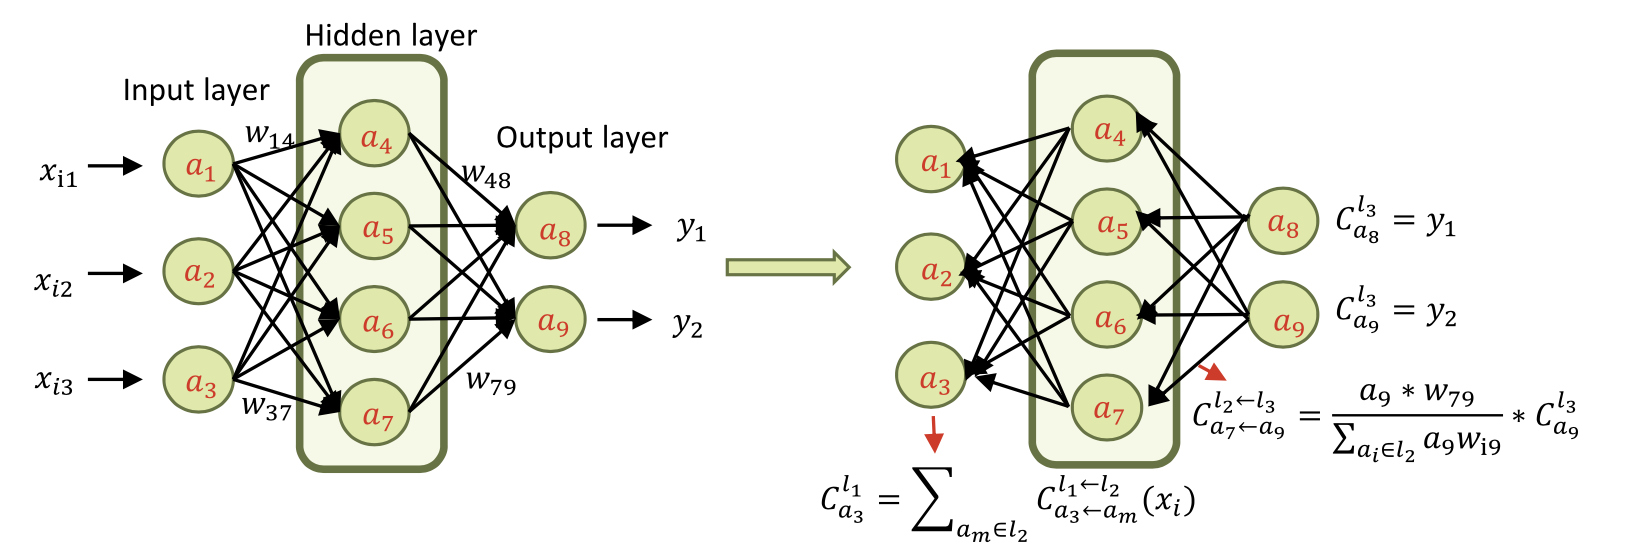
\includegraphics[scale=0.5]{fig2/C3/前向传播算法}%联邦学习的系统架构
	\caption{层间依赖传播算法}
	\label{fig:层间依赖传播算法}	
\end{figure}

根据矩阵层之间的线性相关性,神经元$a_{i}$在第k层的贡献$C_{a_{i}}^{l_{k}}\left(x_{i}\right)$等于连接到神经元$a_{i}$的相邻层的贡献之和:
\begin{equation}\label{eq:层间传播1}
C_{a_{i}}^{l_{k}}\left(x_{i}\right)=\sum_{a_{j} \in l_{k+1}} C_{a_{i} \leftarrow a_{j}}^{l_{k} \leftarrow l_{k+1}}\left(x_{i}\right)
\end{equation}

比如,在图\ref{fig:层间依赖传播算法}中,存在:
\begin{equation}\label{eq:层间传播2}
C_{a_{7}}^{l_{2}}\left(x_{i}\right)=\sum_{a_{j} \in l_{3}} C_{a_{7} \leftarrow a_{j}}^{l_{2} \leftarrow l_{3}}\left(x_{i}\right)=C_{a_{7} \leftarrow a_{8}}^{l_{2} \leftarrow l_{3}}\left(x_{i}\right)+C_{a_{7} \leftarrow a_{9}}^{l_{2} \leftarrow l_{3}}\left(x_{i}\right)
\end{equation}

其中,"←"表示两部分之间的连接关系。具体来说,"l2 ← l3 "是指神经网络中第二层和第三层之间相邻层的连接关系。那么对于第k个输出层:
\begin{equation}
C_{a_{i}}^{l_{k}}\left(x_{i}\right)=f\left(x_{i},\omega_{i}^{r}\right)
\end{equation}

因此,神经元$a_{j}$对于输出层的贡献等于模型的输出。第k层的神经元$a_{j}$对于第k-1层的神经元$C_{a_{i} \leftarrow a_{j}}^{l_{k-1} \leftarrow l_{k}}\left(x_{i}\right)$等于:
\begin{equation}
C_{a_{i} \leftarrow a_{j}}^{l_{k-1} \leftarrow l_{k}}\left(x_{i}\right)=\left\{\begin{array}{cc}\frac{a_{i} w_{i, j}}{\sum_{a_{i} \in l_{k-1} a_{i} w_{i, j}}} C_{a_{j}}^{l_{k}}\left(x_{i}\right) & \sum_{a_{i} \in l_{k-1}} a_{i} w_{i, j} \neq 0 \\ \mu & \sum_{a_{i} \in l_{k-1}} a_{i} w_{i, j}=0\end{array}\right.
\end{equation}

其中$\mu$是一个无限接近于零,但大于零的数字。从上述公式中,我们可以认为每一层的贡献是相等的,而且贡献是逐层传递的。根据以上公式的推导,我们能得到神经网络模型中每一层以及每个神经元的贡献值。


\subsection{自适应噪声添加}
在第二章中介绍了关于神经网络的结构,
\begin{equation}\label{eq:神经网络参数传递}
y=a(\mathbf{x} * \omega+b)
\end{equation}

公式\ref{eq:神经网络参数传递}是学习模型中每个隐藏神经元的转化过程。
其中$\mathbf{x}$代表输入向量,$y$是输出,$b$和$\omega$分别代表偏置项和权重矩阵。$a()$是一个激活函数,用于结合线性变换和非线性变换。$y=a(\mathbf{x} * \omega+b)$ 是线性变换部分。

由于神经网络的结构,上一层的输出是下一层的输入,由此我们可以得出,原始的训练数据只被第一隐层的线性变换所利用。直观地说,为了得到一个具有隐私保护的学习模型,我们可以在第一层隐藏层的数据中注入噪声。正如Phan等人\upcite{ref36}提到的,对于线性变换有一种传统的方法,即向原始数据注入具有相同隐私预算的噪声,但是这容易导致隐私预算增加,并且使原始数据失真过多。因此,本文提出一种自适应噪声添加算法,针对每个梯度计算其贡献值,根据贡献值进行梯度裁剪并添加噪声。

首先,我们引入了两个调整因素$f$和$p$。其中,$f$代表一个阈值,用于决定属性对模型结果输出的贡献是高还是低,其值由用户定义,即贡献超过阈值$f$的属性类对输出的贡献更大。然后,我们向所有这些属性注入自适应拉普拉斯噪声。当贡献率低于阈值$f$时,对这些属性进行概率选择。也就是说,我们选择概率为$1-p$的原始数据,并对一些概率为$p$的属性注入自适应拉普拉斯噪声。该公式如下:
\begin{equation}\label{eq:神经网络加噪}
\tilde{x}_{i, j}=\left\{\begin{array}{ll}
\ddot{x}_{i, j} & \beta \geq f \\
\bar{x}_{i, j} & \beta<f
\end{array}\right.
\end{equation}

其中$\beta$代表贡献率:$\beta=\frac{\left|\ddot{C}_{j}\right|}{\sum_{j=1}^{u}\left|\ddot{C}_{j}\right|}$,当$\beta<f$时,我们有:
\begin{equation}\label{eq:神经网络加噪2}
\bar{x}_{i, j}=\left\{\begin{array}{l}
\ddot{x}_{i, j} \text { with probability } p \\
x_{i, j} \text { with probability } 1-p
\end{array}\right.
\end{equation}


$f$和$p$是超参数,用户可以根据自己的情况来调整。

也就是说,隐私预算$\epsilon_{l}$是根据贡献率:$\epsilon_{j}=\frac{u *\left|\ddot{C}_{j}\right|}{\sum_{j=1}^{u}\left|\ddot{C}_{j}\right|} * \epsilon_{l}$。按比例分配给每个属性类。自适应噪声按以下方式注入属性中:
\begin{equation}\label{eq:神经网络加噪3}
x_{i, j}^{\prime}=x_{i, j}+\frac{1}{\left|D_{i}^{t}\right|} \operatorname{Lap}\left(\frac{G S_{l}}{\epsilon_{j}}\right)
\end{equation}

在不丧失一般性的情况下,调整因子$f$和$p$的值与系统的准确性和隐私水平有关。即$f$越小,$p$越大。越高的秘密水平,准确性越低,反之亦然。

我们采用层间相关性传播算法计算每一层对模型输出的贡献比率。每个用户都在本地对原始数据在神经网络中进行前向传播的训练,这可以获得一个新的数据操作,从而获得本地模型的输出。根据相邻层之间的线性关系,在第k层的神经元的贡献$C_{a_{i}}^{l_{k}}\left(x_{i}\right)$等于连接到神经元$a_{i}$的相邻层的贡献之和:
\begin{equation}\label{eq:神经网络加噪4}
C_{a_{i}}^{l_{k}}\left(x_{i}\right)=\sum_{a_{j} \in l_{k+1}} C_{a_{i} \leftarrow a_{j}}^{l_{k} \leftarrow l_{k+1}}\left(x_{i}\right)
\end{equation}

例如图\ref{fig:层间依赖传播算法}所示,我们有:
\begin{equation}
C_{a_{7}}^{l_{2}}\left(x_{i}\right)=\sum_{a_{j} \in l_{3}} C_{a_{7} \leftarrow a_{j}}^{l_{2} \leftarrow l_{3}}\left(x_{i}\right)=C_{a_{7} \leftarrow a_{8}}^{l_{2} \leftarrow l_{3}}\left(x_{i}\right)+C_{a_{7} \leftarrow a_{9}}^{l_{2} \leftarrow l_{3}}\left(x_{i}\right)
\end{equation}

其中,"$\leftarrow$"表示两部分之间的连接关系。"$l_{2} \leftarrow l_{3}$" 是指深度神经网络中第2层和第3层之间相邻层的连接关系。
当第k层为输出层时,我们有:
\begin{equation}
C_{a_{i}}^{l_{k}}\left(x_{i}\right)=f\left(x_{i}, \omega_{i}^{r}\right)
\end{equation}

\subsection{梯度范数裁剪}
在模型的每一轮迭代过程中,算法将计算添加了高斯噪声的梯度$g=\nabla f+N\left(0, \Delta^{2} \sigma^{2} I\right)$, 方差是 $\sigma^{2}$ 。对梯度注入的噪声量 $\Delta^{2} \sigma^{2}$ 会根据用户个体对于梯度 $g$ 在二范数下的最 大全局敏感度, 即 $\Delta$ 。由于梯度的大小没有一个先验的界限, 我们用二范数的固定值来裁剪每个梯度。

用户上传的梯度向量将可以改写为 $g=g / \max \left(1, \frac{\|g\|}{C}\right)$, 其 中 $C$ 为裁剪阈值。参数裁剪行为确保了梯度值小于 $\mathrm{i}$ 一定的阈值, 即当 $\|g\| \leq C$ 时, 那么 $g$ 保持不变; 当 $\|g\|>C$ 时, 它按比例缩小为 $C_{\circ}$ 可以注意到, 这种形式的梯度裁剪是获得全局灵敏度的常用的方法。

但是参数clip$c$的值如果太小,那么裁剪后的噪声会较小,算法添加的噪声较小时可能会破坏梯度估计的无偏性;但是如果不对梯度进行裁剪,大量的噪声添加到每个梯度会导致模型的可用性大大降低。在模型训练前期,梯度所包含的数据信息更多,因此可以对应添加更多的高丝噪声,使用较大的clip$c$的值,使得梯度裁剪后的模型偏差更小;而在模型训练后期,梯度所包含的数据信息相对较小了,如果还使用相同的clip$c$,会引入很多不必要的噪声。

因此我们根据训练轮数和层间贡献率动态调整裁剪的值。在每次迭代中,该算法使用方差为$sigma^{2}$的高斯机制来计算噪声梯度$g=\nabla f+N\left(0, \sigma^{2} I\right)$。噪声$sigma^{2}$的大小取决于一个个体在$l_{2}$规范下对$g$的最大影响,即$Delta$。由于对梯度的大小没有先验的约束,我们以$l_{2}$规范对每个梯度进行剪辑。因此,梯度向量$g$被$g=g/max \left(1, \frac{\|g\|}{C}\right)$取代,以达到剪裁阈值$C$。这种剪裁保证了如果$|g\| \leq C$,那么$mathrm{g}$将被保留,而如果$|g\|>C$,它将被缩减为准则$C$。

\subsection{解析高斯机制}
高斯机制是差分隐私数据分析算法的基本组成部分。差分隐私的定义可以理解为: 如果删除或者替换数据集中的个体对输出分布的影响可以忽略不计, 那么对私有数据的计算不会泄漏数据集中个体的敏感信息。
在第二章的基础知识中, 我们简要介绍了传统的高斯机制。它的定义如下: 
\begin{define}\label{差分隐私高斯机制}
对于任意 $\varepsilon \in(0,1)$ 与 $c^{2}>2 \ln (1.25 / \delta)$, 高斯噪声参数满足 $\sigma \geq c \Delta_{2} f / \varepsilon$ 的高斯干扰机制为 $(\varepsilon, \delta)$-差分隐私。
\end{define}

在此基础上我们自然的有两个疑问:一是是否定义中的参数 $\sigma$ 是使算法满足 $(\varepsilon, \delta)$-差分隐私的最小值, 即是否可以施加更小的干扰来达到相同的差分隐私保护效果; 二是如果隐私预算 $\varepsilon$ 大于 1 会发生什么。

Balle[文献]等人分析了传统的高斯机制在高隐私保护力度、隐私损失分析、低隐私保护力度三个方面中存在的问题,提出了一种改进的解析高斯机制(Analytic Gaussian Mechanism )。传统的高斯机制施加的噪声干扰过大, 方差公式在高隐私预算下过紧, 并且无法适用于隐私预算大于 1 的低隐私保护力度场景。解析高斯机制针对这些局限性提出了解决方案。

解析高斯机制的核心思想是使用高斯累积分布函数的计算, 来代替传统高斯机制的尾部约束近似。它的定义如下:
\begin{define}\label{解析高斯机制}
令 $f: \mathbb{N}^{\mathbb{N}^{\prime}} \rightarrow \mathbb{R}^{d}$ 表示一个 $\ell_{2}$ 敏感度为 $\Delta_{2}$ 的函数, 对任意 $\varepsilon \geq 0$ 与 $\delta \in[0,1]$, 当且仅当 $\sigma$ 满足下列不等式时, 含参数 $\sigma$ 的高斯机制满足 $(\varepsilon, \delta)$-差分隐私:
\begin{equation}\label{eq:解析高斯机制}
\Phi\left(\frac{\Delta_{2}}{2 \sigma}-\frac{\varepsilon \sigma}{\Delta_{2}}\right)-e^{\varepsilon} \Phi\left(-\frac{\Delta_{2}}{2 \sigma}-\frac{\varepsilon \sigma}{\Delta_{2}}\right) \leq \delta
\end{equation}
\end{define}

其中, $\Phi(t)=(1+\operatorname{erf}(t / \sqrt{2})) / 2$, erf 是高斯误差函数, 即 $\operatorname{erf}(x)=\frac{2}{\sqrt{\pi}} \int_{0}^{x} e^{-\eta^{2}} d \eta$ 。传统的差分隐私高斯机制的干扰大小$\sigma$可以直接计算,解析高斯机制的实现如下算法:

\begin{algorithm}[!htb]
	\caption{解析高斯算法}
	\label{解析高斯算法}
	\begin{algorithmic}[1]
		\footnotesize
		\STATE \textbf{输入:} $f, x, \Delta, \varepsilon, \delta$
		\STATE \textbf{输出:} 干扰后的 $f$
		\STATE 令 $\delta_{0}=\Phi(0)-e^{\varepsilon} \Phi(-\sqrt{2 \varepsilon})$
		\IF{如果 $\delta \geq \delta_{0}$}
			\STATE 定义 $B_{\varepsilon}^{+}(v)=\Phi(\sqrt{\varepsilon v})-e^{\varepsilon} \Phi(-\sqrt{\varepsilon(v+2)})$
			\STATE 计算 $v^{*}=\sup \left\{v \in \mathbb{R}_{\geq 0}: B_{\varepsilon}^{+}(v) \leq \delta\right\}$
            \STATE 令 $\alpha=\sqrt{1+v^{*} / 2}-\sqrt{v^{*} / 2}$
        \ELSE
        	\STATE 定义 $B_{\varepsilon}^{-}(u)=\Phi(-\sqrt{\varepsilon u})-e^{\varepsilon} \Phi(-\sqrt{\varepsilon(u+2)})$
        	\STATE 计算 $u^{*}=\inf \left\{u \in \mathbb{R}_{\geq 0}: B_{\varepsilon}^{-}(u) \leq \delta\right\}$
        	\STATE 令 $\alpha=\sqrt{1+u^{*} / 2}+\sqrt{u^{*} / 2}$
        \ENDIF
    	\STATE 令 $\sigma=\alpha \Delta / \sqrt{2 \varepsilon}$
    	\STATE \textbf{输出:} $f(x)+\mathcal{N}\left(0, \sigma^{2} I\right)$
	\end{algorithmic}
\end{algorithm}


\section{隐私性证明}
自适应差分SGD算法对线性变换函数进行了扰动,该函数满足$\left(\epsilon_{c}+\epsilon_{l}\right)$差分隐私。证明如下:

在贡献中添加的扰动为:
\begin{equation}\label{eq:贡献中添加的噪声}
\ddot{C}_{j}\left(x_{i}\right)=C_{j}\left(x_{i}\right)+\operatorname{Lap}\left(\frac{G S_{c}}{\epsilon_{c}}\right), j \in[1, u]
\end{equation}
它是满足$\epsilon_{c}$-差分隐私的。

贡献$G S_{c}$的敏感度为:
\begin{equation}\label{eq:贡献敏感度}
\begin{aligned}
G S_{c} &=\frac{1}{|D|} \sum_{j=1}^{u}\left\|\sum_{x_{i} \in D} C_{x_{i, j}}\left(x_{i}\right)-\sum_{x_{i}^{\prime} \in D^{\prime}} C_{x_{i, j}^{\prime}}\left(x_{i}^{\prime}\right)\right\|_{1} \\
&=\frac{1}{|D|} \sum_{j=1}^{u}\left\|C_{x_{n, j}}\left(x_{n}\right)-C_{x_{n, j}^{\prime}}\left(x_{n}^{\prime}\right)\right\|_{1} \\
& \leq \frac{2}{|D|} \max \sum_{j=1}^{u}\left\|C_{x_{i, j}}\left(x_{i}\right)\right\|_{1} \\
& \leq \frac{2 u}{|D|}
\end{aligned}
\end{equation}

其中,$u$和$|D|$分别表示贡献的数量和元组,然后可以得到:
\begin{equation}\label{贡献数量和元组}
\begin{aligned}
\frac{\operatorname{Pr}(\ddot{C}(D))}{\operatorname{Pr}\left(\ddot{C}\left(D^{\prime}\right)\right)} &=\frac{\prod_{j=1}^{u} \exp \left(\frac{\epsilon_{c}\left\|\frac{1}{|D|} \sum_{x_{i} \in D} C_{j}\left(x_{i}\right)-\ddot{C}_{j}\left(x_{i}\right)\right\|_{1}}{G S_{c}}\right)}{\prod_{j=1}^{u} \exp \left(\frac{\epsilon_{c}\left\|\frac{1}{\left|D^{\prime}\right|} \sum_{x_{i}^{\prime} \in D^{\prime}} C_{j}\left(x_{i}^{\prime}\right)-\ddot{C}_{j}\left(x_{i}^{\prime}\right)\right\|_{1}}{G S_{c}}\right)} \\
&=\prod_{j=1}^{u} \exp \left(\frac{\epsilon_{c}}{|D| G S_{c}}\left\|C_{j}\left(x_{n}\right)-C_{j}\left(x_{n}^{\prime}\right)\right\|_{1}\right) \\
& \leq \prod_{j=1}^{u} \exp \left(\frac{\epsilon_{c}}{|D| G S_{c}} \max \left\|C_{j}\left(x_{n}\right)\right\|_{1}\right) \\
&=\exp \left(\epsilon_{c} \frac{\max _{x_{i} \in D} \sum_{j=1}^{u}\left\|C_{j}\left(x_{n}\right)\right\|_{1}}{|D| G S_{c}}\right) \\
& \leq \exp \left(\epsilon_{c}\right)
\end{aligned}
\end{equation}

因此,添加噪声后的贡献值是满足$\epsilon_{c}$-差分隐私的。

假设两个相邻的批次$D_{i}^{t}$和$D_{i}^{t^{\prime}}$,其最后一个元组$x_{n}$和$x_{n}^{\prime}$不同,$z\left(D_{i}^{t}\right)$和$z\left(D_{i}^{t^{\prime}}\right)$分别为线性变换函数。

一般来说,我们把偏置项视为第一类数据属性,即:$x_{i,0}=b_{i}$。线性转换可以改写为:$\ddot{\mathbf{z}}_{x \in D_{i}^{t}}(\omega)=\ddot{\mathbf{x}} * \omega$。线性变换的敏感性$G S_{l}$如下:
\begin{equation}
\begin{aligned}
G S_{l} &=\sum_{a_{i} \in l_{1}} \sum_{j=1}^{u}\left\|\sum_{x_{i} \in D_{i}^{t}} x_{i, j}-\sum_{x_{i}^{\prime} \in D_{i}^{t^{\prime}}} x_{i, j}^{\prime}\right\|_{1} \\
&=\sum_{a_{i} \in l_{1}} \sum_{j=1}^{u}\left\|x_{n, j}-x_{n, j}^{\prime}\right\|_{1} \\
& \leq \sum_{a_{i} \in l_{1}} \sum_{j=1}^{u} \max _{x_{i} \in D_{i}^{t}}\left\|x_{n, j}\right\|_{1} \\
& \leq \sum_{a_{i} \in l_{1}} u
\end{aligned}
\end{equation}

其中,$a_{i} \in l_{1}$是指第一隐藏层$l_{1}$中的神经元$a_{i}$,$u$是数据元组$x_{i} \in D_{i}^{t}$中的属性数。它包括两个调整因素:$f$和$p$,它们可以过滤多余的噪声。之后的属性的一般表达式如下:
\begin{equation}
\begin{aligned}
\tilde{x}_{i, j} &=[(1-f)+f * p] * \ddot{x}_{i, j}+f *(1-p) * x_{i, j} \\
&=[(1-f)+f * p]\left[x_{i, j}+\operatorname{Lap}\left(\frac{G S_{l}}{\epsilon_{j}}\right)\right]+[f *(1-p)] x_{i, j} \\
&=x_{i, j}+[(1-f)+f * p]\left[\operatorname{Lap}\left(\frac{G S_{l}}{\epsilon_{j}}\right)\right]
\end{aligned}
\end{equation}
然后我们可以得到:

\begin{equation}
\begin{aligned}
\frac{\operatorname{Pr}\left(\ddot{\mathbf{z}}_{D_{i}^{t}}(\omega)\right)}{\operatorname{Pr}\left(\ddot{\mathbf{z}}_{D_{i}^{t}}(\omega)\right)} &=\frac{\prod_{a_{i} \in l_{1}} \prod_{j=1}^{u} \exp \left(\frac{\epsilon_{j}\left\|\sum_{x_{i} \in D_{i}^{t}} x_{i, j}-\sum_{x_{i} \in D_{i}^{t}} \tilde{x}_{i, j}\right\|_{1}}{G S_{l}}\right)}{\prod_{a_{i} \in l_{1}} \prod_{j=1}^{u} \exp \left(\frac{\epsilon_{j}\left\|\sum_{x_{i}^{\prime} \in D_{i}^{t^{\prime}}} x_{i, j}^{\prime}-\sum_{x_{i}^{\prime} \in D_{i}^{t^{\prime}}} \tilde{x}_{i, j}^{\prime}\right\|_{1}}{G S_{l}}\right)} \\
& \leq \prod_{a_{i} \in l_{1}} \prod_{j=0}^{u} \exp \left(\frac{\epsilon_{j}}{G S_{l}}\left\|\sum_{x_{i} \in D_{i}^{t}} x_{i, j}-\sum_{x_{i}^{\prime} \in D_{i}^{t^{\prime}}} x_{i, j}^{\prime}\right\|_{1}\right) \\
& \leq \prod_{a_{i} \in l_{1}} \prod_{j=0}^{u} \exp \left(\frac{\epsilon_{j}}{G S_{l}} \max _{x_{i} \in D_{i}^{t}}\left\|x_{n, j}\right\|_{1}\right) \\
& \leq \exp \left(\epsilon_{l} \frac{\sum_{a_{i} \in l_{1}} u\left[\sum_{j=1}^{u} \frac{\left|\ddot{C}_{j}\right|}{\sum_{j=1}^{u}\left|\ddot{C}_{j}\right|}\right]}{G S_{l}}\right) \\
&=\exp \left(\epsilon_{l}\right)
\end{aligned}
\end{equation}

根据上述推倒证明可知,在联邦学习的神经网络中添加自适应噪声后,所上传的梯度是满足$\left(\epsilon_{c}+\epsilon_{l}\right)$差分隐私的。在满足差分隐私的基础上,在下一节我们会给出隐私损失累积函数计算隐私成本。

\section{隐私预算分析}
对于本章所提出的在随机梯度下降算法的上进行差分隐私保护算法,除了确保算法运行的准确率以外,另一个重要的问题就是评估算法训练时的数据隐私损失成本。为此,提出隐私损失累积函数的概念来进行每次迭代过程访问训练数据的隐私损失以及随着训练进展时的累积隐私损失。
为不失一般性,令 $\sigma=\frac{\sqrt{2 \log (1.25 / \delta)}}{\varepsilon}$, 文献[36]严格证明,对于抽样概率 $q=\frac{\mathcal{L}}{N}$ 且 $\varepsilon<1$, 则对于完整样本而言,每次迭代过程都是 $(O(q \varepsilon),q \varepsilon)$-差分隐私的。 但文献并末对迭代过程以及噪声强度对差分隐私损失的影响展开研究,故无法对噪声强度以及剪切阈值$C$进行有依据的选取。故首先需要研究迭代过程对差分隐私的影响机制。

事实上,若令 $\sigma \geqslant c_{2} \frac{q \sqrt{T \log (1 / \delta)}}{\varepsilon}$,则同样应用文献[36]方法,可以严格证明算法对于任意的 $\varepsilon<c_{1} q^{2} T$ 都是 $(O(q \varepsilon \sqrt{T}),\delta)-$ 差分隐私的,其中 $c_{1}$ 和 $c_{2}$ 为常数。与文献\upcite{ref36}相比,本文算法能够在相同迭代步骤下,大幅度降低 $\varepsilon$ 的数值,对数据的隐私性保护更高。进一步地, 对于两个相邻的数据集 $d$,$d^{\prime} \in D$ 和映射机制 $M$,引入一个辅助输入变量 aux和输出$o \in R$, 定义映射机制$M$在输出$o$处的隐私损失为:
\begin{equation}
c\left(o ; M, a u x, d, d^{\prime}\right) \triangleq \log \frac{\operatorname{Pr}[M(a u x, d)=o]}{\operatorname{Pr}\left[M\left(a u x, d^{\prime}\right)=o\right]}
\end{equation}

对于所提差分隐私SGD算法而言,神经网络各层权重系数的参数值与每次迭代过程中的差分隐私机制有着紧密的关联,从而对于给定的映射机制 $M$,在第 $\lambda$ 次迭代过程的隐私损失定义为:
\begin{equation}\label{eq:隐私损失定义}
\begin{array}{r}
\alpha_{\mathcal{M}}\left(\lambda ; a u x, d, d^{\prime}\right) \triangleq \log \mathbb{E}_{o \sim M(a u x, d)}[\exp (\lambda c(o) ; M \\
\left.\left.\left.d,d^{\prime}\right)\right)\right]
\end{array}
\end{equation}

进一步地,映射机制 $M$ 的损失边界值定义为:
\begin{equation}\label{eq:损失边界值定义}
\alpha_{\mathcal{M}}(\lambda) \triangleq \max _{a u x, d, d^{\prime}} \alpha_{M}\left(\lambda ; a u x, d, d^{\prime}\right)
\end{equation}

其满足以下特性:

\begin{itemize}
\item 组合特性:给定一个机制 $M$, 由一组子机制顺序 $\left\{M_{1}, M_{2}, \cdots, M_{k}\right\}$ 组成,并满足$M_{i}: \prod_{j=1}^{i-1} R_{j} \times D \rightarrow R_{i}$,从而总隐私损失边界满足:
\begin{equation}\label{eq:损失边界值定义2}
\alpha_{M}(\lambda) \leqslant \sum_{i=1}^{k} \alpha_{M_{i}}(\lambda)
\end{equation}

\item 差分隐私边界:$\forall \varepsilon>0$, 映射机制 $M$ 是 $(\varepsilon,\delta)$ 差分隐私的,当且仅当:
\begin{equation}\label{eq:损失边界值定义2}
\delta=\min _{\lambda} \exp \left(\alpha_{M}(\lambda)-\lambda \varepsilon\right)
\end{equation}
\end{itemize}

上述2条性质确定了深度神经网络算法每次迭代的隐私损失以及所能够达到侵犯数据隐私容忍度的最大迭代次数。特别地,在附加高斯噪声的情况下,不妨令 $\mu_{0}$,$\mu_{1}$ 分别为 $N\left(0,\sigma^{2}\right)$ 和 $N\left(0,\sigma^{2}\right)$ 的概率密度函数,而 $\mu$ 为两个高斯密度函数的混合概率密度函数,即$\mu=(1-q) \mu_{0}+q \mu_{1}$。依据式\ref{eq:隐私损失定义}-\ref{eq:损失边界值定义2}可推导得 $\alpha$ $(\lambda)=\log \max \left(E_{1},E_{2}\right)$, 其中:
\begin{equation}\label{eq:隐私容忍1}
E_{1}=\mathbb{E}_{z \sim \mu_{0}}\left[\left(\frac{\mu_{0}(z)}{\mu(z)}\right)^{\lambda}\right]
\end{equation}

\begin{equation}\label{eq:隐私容忍2}
E_{1}=\mathbb{E}_{z \sim \mu_{0}}\left[\left(\frac{\mu_{0}(z)}{\mu(z)}\right)^{\lambda}\right]
\end{equation}

\section{本章总结}
联邦学习以分布式学习技术为基础,使参与者彼此通过一定的方式(如中心服务器)联合起来训练一个神经网络。在这个过程中,参与者不需要将自己的隐私数据暴露出来便可以参与协作训练,可以克服参与者本地数据集较小、数据样本比较单一、隐私泄露等缺点。虽然基本的分布式协作深度学习没有直接暴露参与者的隐私数据集,但是恶意攻击者仍然可以通过共享的参数等信息获得一定的隐私信息。 

本章详细介绍了基于梯度自适应加噪的差分隐私保护模型对于模型准确度的影响。其中梯度下降作为一种常见的深度学习优化方法,将梯度进行噪声扰动是最早被提出、也是目前相对主流的差分隐私加噪方案之一。我们设计了一个自适应噪声添加的方案,根据贡献率注入不同隐私预算的噪声。与传统的注入噪声的方法相比,我们在相同的隐私保护程度下最大限度地提高了模型的准确性。然后我们采用解析高斯机制计算对其梯度施加的干扰大小,最后分析了模型整体的隐私预算。然而,客户端的匿名性不足以防止侧信道链接攻击,例如,如果客户端在每次迭代中同时上传了大量的权重更新,云仍然可以将它们链接在一起。因此下一章将针对一种训练轮数无关的安全聚合模型进行研究。


\chapter{联邦学习的安全混洗模型}
\label{ch4}
\section{引言}
上一章节中所提出的本地自适应差分隐私方案是通过在客户端将梯度上传至参数服务器前,对梯度添加自适应噪声,尽管方案采用了本地差分技术减少一定程度的隐私预算,但不可避免的会降低联邦学习模型的准确性以及学习效率。正如\upcite{ref37}所指出的,一个复杂的隐私保护系统将多个本地差分隐私的算法进行组合,从而导致这些算法的隐私成本增长。也就是说,隐私预算为ε1和ε2的局部差异化算法的组合会消耗的隐私预算总和为ε1+ε2。使用联邦学习训练的联合模型需要客户在多次迭代中向中央服务器上传梯度更新。如果在迭代训练过程中的每一次迭代都应用本地自适应差分隐私,隐私预算就会累积起来,从而导致总隐私预算的爆炸。现有的本地差分隐私协议对于多维聚集的联邦学习框架可能是不可行的,局部噪声带来的误差会随着维度系数的增加而加剧\upcite{ref38},从而大大降低模型的精度。而且,当参与一次迭代的客户端数量达到上千人时,会导致聚合任务升级成一个高维任务,隐私预算暴增。
而且,值得关注的是,不同的用户有不同的隐私需求,不同的用户上传的梯度对于联合模型的贡献比也有差异,因此本章将提出混合差分隐私技术,构造一个全新的可信第三方——混洗器,与本地差分隐私相结合,实现的方案能提高全局模型的精度,也保证在更低的隐私成本下达到相同的隐私预算。

在本章节中我们提出了一个在联邦学习中的安全混洗器,本地客户端使用自适应差分隐私对于模型的输出进行加躁,然后安全混洗器从客户端上传的样本中随机采样,将收集到的梯度以维度进行拆分,打乱次序,达到隐私放大效果,再采用梯度稀疏化的技术筛选对联合模型贡献较高的梯度,发送给中央服务器进行聚合。安全混洗器作为一个可信第三方,独立于服务器并专门用于本地客户端梯度的子采样、混洗、上传。这个模型通过子采样和混洗两者的结合达到隐私放大效应,从而提高了整体联邦学习模型的精度。当本地差分隐私添加更少的噪音时,对于同样的中央服务器能达到相同水平的隐私预算。

我们将在本章节详细的描述该框架中各个模块的设计和实现过程。

\section{安全混洗模型}
如图\ref{fig:联邦学习中的安全模型框架}所示,该框架主要由本地客户端、混洗器和中央服务器3部分组成:
\begin{itemize}
  \item 本地客户端: 基于第三章的本地自适应差分隐私方案,在模型训练的梯度下降算法中对梯度进行自适应的扰动,得到满足$\left(\epsilon_{c}+\epsilon_{l}\right)$差分隐私的梯度。
  \item 混洗器: 一个半诚信的第三方。首先动态采样本地客户端上传的梯度,然后借助现有的安全混洗协议在对数据一无所知的情况下,对子采样后的梯度完成安全的拆分混洗操作,通过隐私放大效应使得算法满足$\epsilon_{0}$-差分隐私,达到梯度匿名机制,最后将混洗后的结果发送至中央服务器。
  \item 中央服务器: 一个诚实但好奇的第三方。服务器接受混洗器上传的梯度并进行聚合,然后更新全局模型。
\end{itemize}

假设现在有m个本地客户端,每个客户端表示为$i \in[m]$,有本地数据集\\$\mathcal{D}_{i}=\left\{d_{i 1}, \ldots, d_{i r}\right\} \in \mathbb{S}^{r}$,由$r$ 个数据集合构成。$F_{i}(\theta)$表示在客户端$i$的本地数据集 $\mathcal{D}_{i}$上进行训练,对于模型梯度$\theta \in \mathbb{R}^{d}$进行衡量的损失函数,其中$F_{i}(\theta)=\frac{1}{r} \sum_{j=1}^{r} f\left(\theta ; d_{i j}\right)$,$f(\theta ; \cdot): \mathcal{C} \rightarrow \mathbb{R}$是凸函数。中央服务器的目标是找到一个最佳的模型参数向量$\theta^{*} \in \mathcal{C}$ 使得损失函数$\min _{\theta \in \mathcal{C}}\left(F(\theta)=\frac{1}{m} \sum_{i=1}^{m} F_{i}(\theta)\right)$最小,其中隐私性满足单个客户端的隐私预算,也就是满足$\epsilon_{0}$-LDP。在算法\ref{联邦学习中的安全模型算法}中,首先我们从m个客户端中随机挑选k个客户端,表示为集合$\mathcal{U}_{t}$,其中$k \leq m$。每个客户端$i \in \mathcal{U}_{t}$从本地数据集中抽样$\mathcal{S}_{i t}$个样本训练模型,计算梯度$\nabla_{\theta_{t}} f\left(\theta_{t} ; d_{i j}\right)$。第$i$个客户端采用基于第三章的自适应本地差分隐私方案,添加噪声、裁剪梯度,然后将梯度发送给混洗器。混洗器对收到的梯度进行拆分混洗,然后发送给中央服务器。最后,中央服务器对混洗后的梯度进行聚合求均值,更新全局模型。

\begin{algorithm}[!htb]
	\caption{联邦学习中的安全模型算法:$\mathcal{A}_{\text {csdp}}$}
	\label{联邦学习中的安全模型算法}
	\begin{algorithmic}[1]
		\footnotesize
		\STATE \textbf{输入:} 数据集$\mathcal{D} \quad=\bigcup_{i \in[m]} \mathcal{D}_{i}$, $\mathcal{D}_{i}=\left\{d_{i 1}, \ldots, d_{i r}\right\}$, loss function $F(\theta)=$ $\frac{1}{m r} \sum_{i=1}^{m} \sum_{j=1}^{r} f\left(\theta ; d_{i j}\right)$,本地差分隐私预算$\epsilon_{0}$,梯度范数阈值$C$,模型学习率$\eta_{t}$
		\STATE \textbf{初始化:} $\theta_{0} \in \mathcal{C}$
		\FOR{$t \in[T]$}
			\STATE \textbf{客户端采样:} 混洗器从k个客户端中随机采样$i \in \mathcal{U}_{t}$个客户端
			\FOR{客户端$i \in \mathcal{U}_{t}$}
				\STATE \textbf{梯度选择:} 客户端i从s个样本空间中随机采样$\mathcal{S}_{i t}$个梯度
				\FOR{样本$j \in \mathcal{S}_{i t}$}
					\STATE $\mathbf{g}_{t}\left(d_{i j}\right) \leftarrow \nabla_{\theta_{t}} f\left(\theta_{t} ; d_{i j}\right)$
					\STATE ${\mathbf{g}}_{t}\left(d_{i j}\right) \leftarrow \mathbf{g}_{t}\left(d_{i j}\right) / \max \left\{1, \frac{\left\|\mathbf{g}_{t}\left(d_{i j}\right)\right\|_{p}}{C}\right\}^{3}$
					\STATE $\mathbf{q}_{t}\left(d_{i j}\right) \leftarrow \mathcal{R}_{p}\left(\tilde{\mathbf{g}}_{t}\left(d_{i j}\right)\right)$
				\ENDFOR
				\STATE 客户端i将$\left\{\mathbf{q}_{t}\left(d_{i j}\right)\right\}_{j \in \mathcal{S}_{i t}}$发送给混洗器
			\ENDFOR
			\STATE \textbf{混洗器:} 混洗器对于$\left\{\boldsymbol{q}_{t}\left(d_{i j}\right): i \in \mathcal{U}_{t}, j \in \mathcal{S}_{i t}\right\}$中的权重进行拆分混洗,然后上传给中央服务器
			\STATE \textbf{中央服务器聚合梯度:}$\overline{\mathbf{g}}_{t} \leftarrow \frac{1}{k s} \sum_{i \in \mathcal{U}_{t}, j \in \mathcal{S}_{i t}} \boldsymbol{q}_{t}\left(d_{i j}\right)$
			\STATE \textbf{梯度下降:}$\theta_{t+1} \leftarrow \prod_{\mathcal{C}}\left(\theta_{t}-\eta_{t} \overline{\mathbf{g}}_{t}\right)$
		\ENDFOR
		\STATE \textbf{输出:}最终全局模型参数$\theta_{T}$

	\end{algorithmic}
\end{algorithm}

\begin{figure}[!hbt]
\centering
	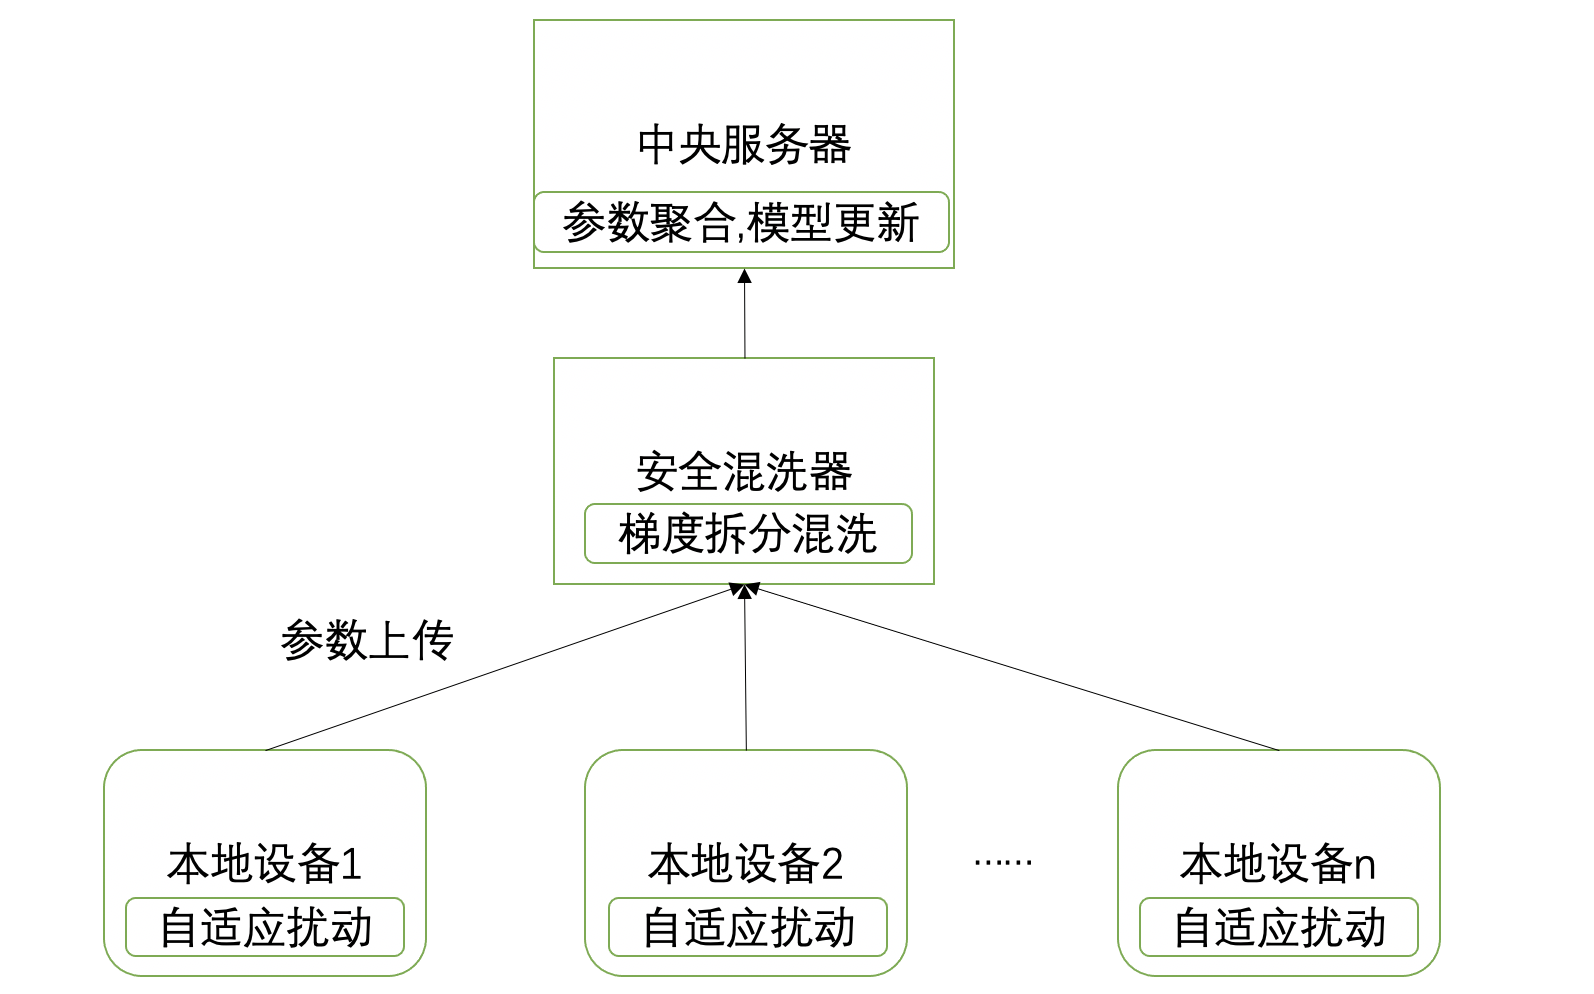
\includegraphics[scale=0.5]{fig2/C4/shuffle模型}%联邦学习的系统架构
	\caption{联邦学习中的安全模型框架}
	\label{fig:联邦学习中的安全模型框架}	
\end{figure}

\subsection{客户端抽样}
假设在空间$\mathcal{U}$中我们有一个数据集$\mathcal{D}^{\prime}=\left\{U_{1}, \ldots, U_{r_{1}}\right\} \in \mathcal{U}^{r_{1}}$,其中包含$r_{1}$个样本元素。如定义\ref{子采样}所示,本文定义一个子采样程序:首先采样一个客户端数据集$\mathcal{D}^{\prime} \in \mathcal{U}^{r_{1}}$,再从中采样一个子集作为客户端的本地训练数据。
\begin{define}[子采样]\label{子采样}
定义一个抽样程序$\operatorname{samp}_{r_{1}, r_{2}}: \mathcal{U}^{r_{1}} \rightarrow \mathcal{U}^{r_{2}}$,其中$r_{2} \leq r_{1}$:从输入的数据集$\mathcal{D}^{\prime} \in \mathcal{U}^{r_{1}}$ 中以随机概率抽选一个子数据集$\mathcal{D}^{\prime \prime}$,数据集$\mathcal{D}^{\prime}$中的每个元素在数据集$\mathcal{D}^{\prime \prime}$中出现的概率为$q=\frac{r_{2}}{r_{1}}$。
\end{define}

\subsection{混洗器}
先前的研究工作(H Brendan McMahan, Daniel Ra- mage, Kunal Talwar, and Li Zhang. Learning differen- tially private recurrent language models. arXiv preprint arXiv:1710.06963, 2017.)表明,在联邦学习模型中,假如在某个时间段数据是被适当的匿名化,并将数据之间的耦合信息拆分后,模型整体的隐私保障可以得到极大的改善。在第三章中的隐私保护方案是基于本地客户端训练数据的,而面对恶意的中央服务器甚至是恶意的第三方攻击者时,无法保障每个客户端的隐私。

因此在本章中,我们针对客户端上传的梯度,进行参数的拆分混洗,通过混洗器达到客户端的匿名性,打破从中央服务器接收的数据与特定客户端之间的联系,并在每次迭代中从同一客户端发送的梯度更新中将信息解耦。

客户端的匿名性可以通过现有的多种机制来实现,这取决于中央服务器在特定场景下如何跟踪客户端。作为一个典型的保护隐私的最佳做法,每个客户对服务器有一定程度的匿名性,以使客户的个人身份识别与他们的权重更新无法关联。例如,如果服务器通过IP地址追踪客户,每个客户可以通过使用网络代理、VPN服务[Belesi, 2016]、公共WiFi接入[Dingledine等人,2004]产生一个无法追踪的IP地址。再比如,如果服务器通过软件生成的元数据(如ID)来追踪客户,每个客户可以在向服务器发送元数据之前将其随机化。

但是,我们认为,客户端的匿名性不足以防止通信链道的攻击。例如,如果客户端在每次迭代中同时上传了大量的权重更新,中央服务器仍然可以将它们连接在一起。因此,我们设计了混洗器,以打破来自相同客户的模型权重更新之间的联系,并将其放置于客户端上传梯度更新至中央服务器之间,使中央服务器更难结合多个客户端的同步更新来推断任何客户的更多信息。

如下图所示,我们的混洗器通过以下步骤对客户端上传的梯度参数进行混洗,然后上传给中央服务器:
\begin{itemize}
	\item 权重分割:每个客户端都对其本地模型的权重进行分割,但给每个分割后的元素贴上一个id,以表明其在网络结构中的权重位置。
	\item 权重混洗:对于所有客户端分割后的权重采用随机扰动机制进行混洗。
\end{itemize}

\begin{figure}[!hbt]
\centering
	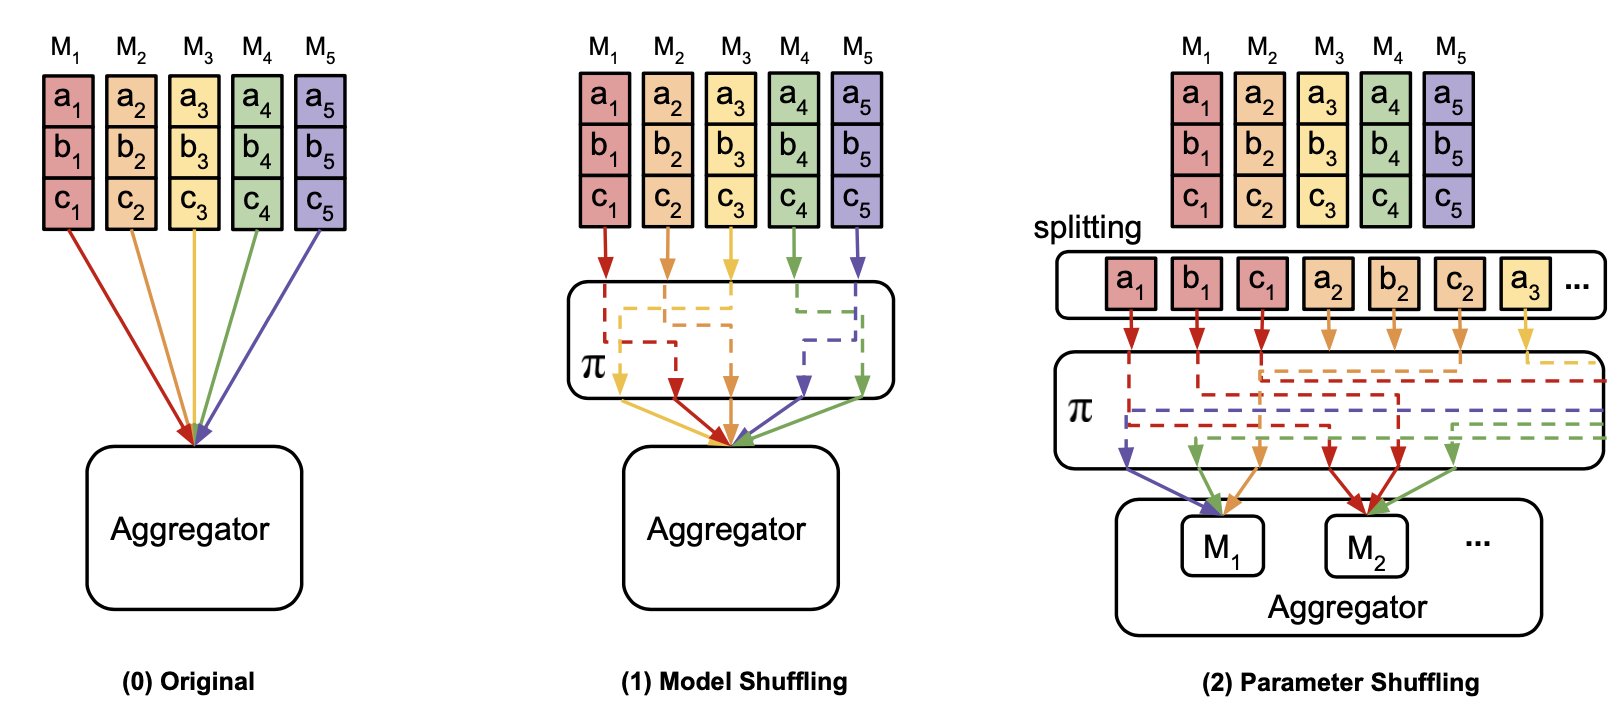
\includegraphics[scale=0.4]{fig2/C4/混洗器}%联邦学习的系统架构
	\caption{联邦学习安全模型中执行参数拆分混洗的混洗器}
	\label{fig:联邦学习安全模型中执行参数拆分混洗的混洗器}	
\end{figure}

\begin{algorithm}[!htb]
	\caption{混洗器中的拆分混洗算法}
	\label{混洗器中的拆分混洗算法}
	\begin{algorithmic}[1]
		\footnotesize
		\STATE \textbf{Input:} 本地客户端添加自适应扰动后的权重$W_{l+1}^{s}$
	    \STATE 对权重$W_{l+1}^{s}$进行分割,给每个元素分配id
	    \FOR{$w^{s} \in W$}
	    \STATE 用一个唯一的id标记元素的位置
	    \STATE 在通信时刻(0,$T$)期间随机采样$t_{i d}^{s} \leftarrow U(0, T) \%$
	    \ENDFOR
	    \STATE 在时刻 $t_{i d}^{s}$将梯度$(i d, w_{i d})$发送给中央服务器
	\end{algorithmic}
\end{algorithm}


\section{隐私放大效应}
隐私放大(privacy amplification)是本章所提出的安全框架中混洗器对隐私效果增强的理论分析,基于该理论,可将现有的本地化差分隐私方法直接应用在安全框架上。

在算法\ref{联邦学习中的安全模型算法}中,每个本地客户端采用第三章的满足$\left(\epsilon_{c}+\epsilon_{l}\right)$的自适应本地差分隐私算法,将参数上传至混洗器进行拆分混洗后,所获取的数据满足 $\varepsilon_{\mathrm{c}}-\mathrm{DP}$。从 $\left(\epsilon_{c}+\epsilon_{l}\right)$到 $\varepsilon_{\mathrm{c}}$ 的转变可通过隐私放大理论证明。$\left(\epsilon_{c}+\epsilon_{l}\right)$ 对应于较大的数值, 表示较低的隐私性; $\varepsilon_{\mathrm{c}}$ 对应于较小的数值, 表示较高的隐私性。因此经过混洗器后,隐私性得到了增强。由差分隐私的强组合性可保证算法$\mathcal{A}_{\text {csdp}}$在每次迭代中对每个样本$d_{i j}$都能保证$\epsilon_{0}$的本地差异隐私。因此本节只需要分析采样和混洗操作的隐私放大性。

\begin{theorem}\label{隐私性证明}
算法\ref{联邦学习中的安全模型算法}是满足$(\epsilon, \delta)-$差分隐私的,当对于任意$\delta$,$\delta>0$ ,并且有:
$$
\epsilon=\mathcal{O}\left(\epsilon_{0} \sqrt{\frac{q T \log (2 q T / \delta) \log (2 / \delta)}{n}}\right)
$$
\end{theorem}

假设在联邦学习模型中,需要迭代的次数为$t \in[T]$。$\mathcal{M}_{t}\left(\theta_{t}, \mathcal{D}\right)$表示在时刻$t$对于数据集$\mathcal{D}$和模型参数为$\theta_{t}$的差分隐私机制,$\theta_{t+1}$表示模型的输出。因此,在数据集$\mathcal{D}=\bigcup_{i=1}^{m} \mathcal{D}_{i} \in \mathfrak{S}^{n}$上的差分隐私机制定义如下:

\begin{equation}\label{eq:隐私性证明机制}
\mathcal{M}_{t}\left(\theta_{t} ; \mathcal{D}\right)=\mathcal{H}_{k s} \circ \operatorname{samp}_{m, k}\left(\mathcal{G}_{1}, \ldots, \mathcal{G}_{m}\right)
\end{equation}

其中,$\mathcal{G}_{i}=\operatorname{samp}_{r, s}\left(\mathcal{R}\left(\boldsymbol{x}_{i 1}^{t}\right), \ldots, \mathcal{R}\left(\boldsymbol{x}_{i r}^{t}\right)\right)$并且$\boldsymbol{x}_{i j}^{t}=$$\nabla_{\theta_{t}} f\left(\theta_{t} ; d_{i j}\right), \forall i \in[m], j \in[r]$。$\mathcal{H}_{k s}$表示在$k s$个数据样本上进行混洗操作, $\operatorname{samp}_{a, b}$表示从有a个元素的集合中随机抽样b个元素的操作。

接下来我们给出$\mathcal{M}_{t}$的隐私性证明:

假设客户端$i \in[m]$的本地数据集为$\mathcal{D}_{i}=\left\{d_{i 1}, d_{i 2}, \ldots, d_{i r}\right\} \in \mathfrak{S}^{r}$,$\mathcal{D}=\bigcup_{i=1}^{m} \mathcal{D}_{i}$表示总体数据集。根据公式\ref{eq:隐私性证明机制},$\mathcal{Z}\left(\mathcal{D}^{(t)}\right)=\mathcal{H}_{k s}\left(\mathcal{R}\left(\boldsymbol{x}_{1}^{t}\right), \ldots, \mathcal{R}\left(\boldsymbol{x}_{k s}^{t}\right)\right)$表示在本地客户端进行本地差分隐私后输出的$ks$个权重集合上进行混洗后的权重。任取$\tilde{\delta}>0$,当$\epsilon_{0} \leq \frac{\log (k s / \log (1 / \tilde{\delta}))}{2}$时,算法$\mathcal{Z}$ 满足 $(\tilde{\epsilon}, \tilde{\delta})-\mathrm{DP}$差分隐私,可得:

\begin{equation}\label{eq:隐私性证明机制2}
\tilde{\epsilon}=\mathcal{O}\left(\min \left\{\epsilon_{0}, 1\right\} e^{\epsilon_{0}} \sqrt{\frac{\log (1 / \tilde{\delta})}{k s}}\right)
\end{equation}

当$\epsilon_{0}=\mathcal{O}(1)$时,有$\tilde{\epsilon}=\mathcal{O}\left(\epsilon_{0} \sqrt{\frac{\log (1 / \tilde{\delta})}{k s}}\right)$。

令$\mathcal{T} \subseteq\{1, \ldots, m\}$表示在时刻$t$选取的k个客户端。对于$i \in \mathcal{T}$,$\mathcal{T}_{i} \subseteq\{1, \ldots, r\}$表示在时刻$t$客户端$i$所抽样的$s$条数据样本。对于任意的 $\mathcal{T} \in\left(\begin{array}{c}{[m]} \\ k\end{array}\right)$和$\mathcal{T}_{i} \in\left(\begin{array}{c}{[r]} \\ s\end{array}\right), i \in \mathcal{T}$,有$\overline{\mathcal{T}}=\left(\mathcal{T}, \mathcal{T}_{i}, i \in \mathcal{T}\right), \mathcal{D}^{\mathcal{T}_{i}}=\left\{d_{j}: j \in \mathcal{T}_{i}\right\}$ for $i \in \mathcal{T}$, and $\mathcal{D}^{\bar{\top}}=\left\{\mathcal{D}^{\mathcal{T}_{i}}: i \in \mathcal{T}\right\}$。$\mathcal{T}$和$\mathcal{T}_{i}, i \in \mathcal{T}$为抽样产生的任意子集,其中的随机性由客户端抽样和数据集抽样所决定。算法$\mathcal{M}_{t}$可以等价的表示为$\mathcal{M}_{t}=\mathcal{Z}\left(\mathcal{D}^{\overline{\mathcal{T}}}\right)$。

假设现有数据集:$\mathcal{D}^{\prime}=\left(\mathcal{D}_{1}^{\prime}\right) \bigcup\left(\cup_{i=2}^{m} \mathcal{D}_{i}\right) \in \mathfrak{S}^{n}$,其中数据集$\mathcal{D}_{1}^{\prime}=\left\{d_{11}^{\prime}, d_{12}, \ldots, d_{1 r}\right\}$和$\mathcal{D}_{1}$ 为相邻数据集,它们的第$d_{11}$条和第$d_{11}^{\prime}$条数据样本不同。如果$\mathcal{M}_{t}$是满足$(\bar{\epsilon}, \bar{\delta})-\mathrm{DP}$差分隐私的,那么对于算法$\mathcal{M}_{t}$所选的任意子集$\mathcal{S}$ 都应该满足:
\begin{equation}\label{eq:隐私性证明3}
\operatorname{Pr}\left[\mathcal{M}_{t}(\mathcal{D}) \in \mathcal{S}\right] \leq e^{\bar{\epsilon}} \operatorname{Pr}\left[\mathcal{M}_{t}\left(\mathcal{D}^{\prime}\right) \in \mathcal{S}\right]+\bar{\delta}
\end{equation}

\begin{equation}\label{eq:隐私性证明4}
\operatorname{Pr}\left[\mathcal{M}_{t}\left(\mathcal{D}^{\prime}\right) \in \mathcal{S}\right] \leq e^{\bar{\epsilon}} \operatorname{Pr}\left[\mathcal{M}_{t}(\mathcal{D}) \in \mathcal{S}\right]+\bar{\delta}
\end{equation}

由于式\ref{eq:隐私性证明3}和\ref{eq:隐私性证明4}是对称的,因此只需要证明其中一条。下文给出式\ref{eq:隐私性证明3}的证明:

令$q=\frac{k s}{m r}$,我们给出条件概率的定义:
\begin{equation}\label{eq:隐私性证明5}
\begin{array}{l}
A_{11}=\operatorname{Pr}\left[\mathcal{Z}\left(\mathcal{D}^{\overline{\mathcal{T}}}\right) \in \mathcal{S} \mid 1 \in \mathcal{T} \text { and } 1 \in \mathcal{T}_{1}\right] \\
A_{11}^{\prime}=\operatorname{Pr}\left[\mathcal{Z}\left(\mathcal{D}^{\prime} \overline{\mathcal{T}}\right) \in \mathcal{S} \mid 1 \in \mathcal{T} \text { and } 1 \in \mathcal{T}_{1}\right] \\
A_{10}=\operatorname{Pr}\left[\mathcal{Z}\left(\mathcal{D}^{\overline{\mathcal{T}}}\right) \in \mathcal{S} \mid 1 \in \mathcal{T} \text { and } 1 \notin \mathcal{T}_{1}\right]=\operatorname{Pr}\left[\mathcal{Z}\left(\mathcal{D}^{\prime \overline{\mathcal{T}}}\right) \in \mathcal{S} \mid 1 \in \mathcal{T} \text { and } 1 \notin \mathcal{T}_{1}\right] \\
A_{0}=\operatorname{Pr}\left[\mathcal{Z}\left(\mathcal{D}^{\bar{T}}\right) \in \mathcal{S} \mid 1 \notin \mathcal{T}\right]=\operatorname{Pr}\left[\mathcal{Z}\left(\mathcal{D}^{\prime \bar{\tau}}\right) \in \mathcal{S} \mid 1 \notin \mathcal{T}\right]
\end{array}
\end{equation}

令$q_{1}=\frac{k}{m}$,$q_{2}=\frac{s}{r}$,那么$q=q_{1} q_{2}$,然后可以得到:
\begin{equation}\label{eq:隐私性证明6}
\begin{aligned} 
\operatorname{Pr}\left[\mathcal{M}_{t}(\mathcal{D}) \in \mathcal{S}\right] &=q A_{11}+q_{1}\left(1-q_{2}\right) A_{10}+\left(1-q_{1}\right) A_{0}
\end{aligned}
\end{equation}

\begin{equation}\label{eq:隐私性证明7}
\begin{aligned} 
\operatorname{Pr}\left[\mathcal{M}_{t}\left(\mathcal{D}^{\prime}\right) \in \mathcal{S}\right] &=q A_{11}^{\prime}+q_{1}\left(1-q_{2}\right) A_{10}+\left(1-q_{1}\right) A_{0} 
\end{aligned}
\end{equation}

因此,我们可以得到:
\begin{equation}\label{隐私性证明8}
A_{11} \leq e^{\tilde{\epsilon}} A_{11}^{\prime}+\tilde{\delta}
\end{equation}

\begin{equation}\label{隐私性证明9}
A_{11} \leq e^{\tilde{\epsilon}} A_{10}+\tilde{\delta}
\end{equation}
式\ref{eq:隐私性证明7}成立,因此混洗器$\mathcal{M}_{t}$是满足$\varepsilon_{\mathrm{c}}$-差分隐私的。

\section{模型收敛性分析}
回顾第二章的基础知识,在随机梯度下降算法的每次迭代中,中央服务器将当前的参数向量发送给所有本地客户端,客户端收到后在本地数据集上进行模型训练,计算随机梯度并上传给中央服务器,然后中央服务器计算收到的梯度的平均值/平均数并更新参数向量。因此在本节中,我们分析采用采样和混洗算法后模型的收敛性。

在算法\ref{联邦学习中的安全模型算法}中,在每一轮迭代过程中,中央服务器聚合上传的$ks$个加躁后的梯度,如算法\ref{联邦学习中的安全模型算法}的第15行所示,中央服务器进行聚合后得到结果:$\overline{\mathbf{g}}_{t} \leftarrow \frac{1}{k s} \sum_{i \in \mathcal{U}_{t}, j \in \mathcal{S}_{i t}} \boldsymbol{q}_{t}\left(d_{i j}\right)$,然后通过随机梯度下降算法更新全局模型参数:$\theta_{t+1} \leftarrow \prod_{\mathcal{C}}\left(\theta_{t}-\eta_{t} \overline{\mathbf{g}}_{t}\right)$。其中,$\mathbf{q}_{t}\left(d_{i j}\right)=\mathcal{R}_{p}\left(\nabla_{\theta_{t}} f\left(\theta_{t} ; d_{i j}\right)\right)$。

既然随机机制$\mathcal{R}_{p}$是无偏的,那么平均梯度$\overline{\mathbf{g}}_{t}$也是无偏的,也就是说,我们有 $\mathbb{E}\left[\overline{\mathbf{g}}_{t}\right]=\nabla_{\theta_{t}} F\left(\theta_{t}\right)$,其中期望是相对于客户端和数据点的随机抽样以及机制$\mathcal{R}_{p}$的随机性而言的。

令$F(\theta)$为凸函数,考虑这样一个随机梯度下降算法:$\theta_{t+1} \leftarrow \prod_{\mathcal{C}}\left(\theta_{t}-\eta_{t} \mathbf{g}_{t}\right)$,$\mathbf{g}_{t}$满足$\mathbb{E}\left[\mathbf{g}_{t}\right]=\nabla_{\theta_{t}} F\left(\theta_{t}\right)$并且$\mathbb{E}\left\|\mathbf{g}_{t}\right\|_{2}^{2} \leq G^{2}$。当确定$\eta_{t}=\frac{D}{G \sqrt{t}}$,可以得到:
\begin{equation}\label{eq:模型收敛性证明1}
\mathbb{E}\left[F\left(\theta_{T}\right)\right]-F\left(\theta^{*}\right) \leq 2 D G \frac{2+\log (T)}{\sqrt{T}}=\mathcal{O}\left(D G \frac{\log (T)}{\sqrt{T}}\right)
\end{equation} 

由文献的证明可知,算法\ref{联邦学习中的安全模型算法}的输出$\theta_{T}$满足:
\begin{equation}\label{eq:模型收敛性证明2}
\mathbb{E}\left[F\left(\theta_{T}\right)\right]-F\left(\theta^{*}\right) \leq \mathcal{O}\left(\frac{L D \log (T) \max \left\{d^{\frac{1}{2}-\frac{1}{p}}, 1\right\}}{\sqrt{T}}\left(1+\sqrt{\frac{c d}{q n}}\left(\frac{e^{\epsilon_{0}}+1}{e^{\epsilon_{0}}-1}\right)\right)\right)
\end{equation}

其中,存在$\sqrt{1+\frac{c d}{q n}\left(\frac{e^{\epsilon_{0}}+1}{e^{\epsilon_{0}}-1}\right)^{2}} \leq\left(1+\sqrt{\frac{c d}{q n}}\left(\frac{e^{\epsilon_{0}}+1}{e^{\epsilon_{0}-1}}\right)\right)$。

当$\sqrt{\frac{c d}{q n}}\left(\frac{e^{\epsilon_{0}}+1}{e^{\epsilon_{0}-1}}\right) \leq \mathcal{O}(1)$时,我们恢复了没有隐私性的虚构SGD的收敛率。而当$\sqrt{\frac{c d}{q n}}\left(\frac{e^{\epsilon_{0}}+1}{e^{\epsilon_{0}}-1}\right) \geq \Omega(1)$时,可以推导出:
\begin{equation}\label{eq:模型收敛性证明3}
\mathbb{E}\left[F\left(\theta_{T}\right)\right]-F\left(\theta^{*}\right) \leq \mathcal{O}\left(\frac{L D \log (T) \max \left\{d^{\frac{1}{2}-\frac{1}{p}}, 1\right\}}{\sqrt{T}} \sqrt{\frac{c d}{q n}}\left(\frac{e^{\epsilon_{0}}+1}{e^{\epsilon_{0}}-1}\right)\right)
\end{equation}

如果我们在算法\ref{联邦学习中的安全模型算法}中设置学习率为$\eta_{t}=\frac{D}{G \sqrt{t}}$,其中\\$G^{2}=$ $L^{2} \max \left\{d^{1-\frac{2}{p}}, 1\right\}\left(1+\frac{c d}{q n}\left(\frac{e^{\epsilon_{0}}+1}{e^{\epsilon_{0}-1}}\right)^{2}\right)$。那么:

\begin{equation}\label{eq:模型收敛性证明4}
\mathbb{E}\left[F\left(\theta_{T}\right)\right]-F\left(\theta^{*}\right) \leq \\
\mathcal{O}\left(\frac{L D \log (T) \max \left\{d^{\frac{1}{2}-\frac{1}{p}}, 1\right\}}{\sqrt{T}} \sqrt{\frac{c d}{q n}}\left(\frac{e^{\epsilon_{0}}+1}{e^{\epsilon_{0}}-1}\right)\right)
\end{equation}

其中,当$p \in\{1, \infty\}$时,$c=4$否则$c=14$。

\begin{theorem}[随机梯度下降算法的收敛性]\label{随机梯度下降算法的收敛性}
假使有凸函数$F(\theta)$,数据集$D$的维度为$\mathcal{C}$,在模型训练过程中采用随机梯度下降算法$\theta_{t+1} \leftarrow \prod_{\mathcal{C}}\left(\theta_{t}-\eta_{t} \mathbf{g}_{t}\right)$,其中 $\mathbf{g}_{t}$满足$\mathbb{E}\left[\mathbf{g}_{t}\right]=\nabla_{\theta_{t}} F\left(\theta_{t}\right)$并且$\mathbb{E}\left\|\mathbf{g}_{t}\right\|_{2}^{2} \leq G^{2}$。当$\eta_{t}=$ $\frac{D}{G \sqrt{t}}$,$\mathbb{E}\left[F\left(\theta_{T}\right)\right]-F\left(\theta^{*}\right) \leq 2 D G\left(\frac{2+\log (T)}{\sqrt{T}}\right)$成立。
\end{theorem}

根据文献中已有的标准随机梯度下降算法收敛结果中使用的\ref{随机梯度下降算法的收敛性}对$G^{2}$的约束条件,证明了混洗算法可在$G^{2}=$ $L^{2} \max \left\{d^{1-\frac{2}{p}}, 1\right\}\left(1+\frac{c d}{q n}\left(\frac{e^{\epsilon_{0}}+1}{e^{\epsilon_{0}-1}}\right)^{2}\right)$时达到全局最优解。

\section{本章总结}
本章节我们针对联邦学习模型的整体框架进行了隐私性改进,提出了安全混洗模型,在本地客户端和中央服务器之间加设混洗器,通过对本地客户端进行随机抽样,将上传的梯度进行拆分混洗,增加隐私放大效果。然后发送给中央服务器进行聚合。并对方案进行了隐私性证明,表明此安全混洗算法可以保证$\varepsilon_{\mathrm{c}}$的差分隐私,然后对此方案在中央服务器上的随机梯度下降算法进行了收敛性的分析,证明在凸函数上,梯度$\mathbf{g}_{t}$满足$\mathbb{E}\left[\mathbf{g}_{t}\right]=\nabla_{\theta_{t}} F\left(\theta_{t}\right)$时模型能达到全局收敛。本章所提出的方案能在保持模型收敛性的情况下,减少隐私预算。



% \chapter{实验与评估}
\label{ch5}
之前的的章节中,我们描述了联邦学习的本地自适应差分隐私和安全混洗模型的设计和实现过程。在本节的内容中,我们选取了一些基准的数据集在该验证框架上进行实验评估。本实验是关于联邦学习系统的隐私保护方案。本章的实验主要针联邦深度学习系统训练样本的攻击模型,保护联邦学习系统中参与者的共享梯度信息,避免梯度参数泄露隐私和恶意服务器获取客户端的信息,进而保护参与者本地训练样本。在实验室环境下,通过多 GPU 虚拟化设置模拟分布式联邦学习系统,并且将差分隐私保护方案和混洗器配置在模拟分布式联邦学习系统中,同时在系统中设置攻击模型,评估满足隐私保护算法的系统学习准确率和隐私保护预算。 
\section{基准数据集介绍}
我们选用了以下三个数据集评估了我们的联邦学习隐私保护框架:
\begin{enumerate}
	\item [(1)] 手写体数字识别数据集(MNIST)\upcite{ref46}是用于分类任务的经典数据集,来源于美国国家标准与技术研究所。总共包含了70000个手写数字图像,每个图像的尺寸为28 x 28像素,每个像素点用灰度值表示,灰度值范围为0到255,图像分为10类别,分别代表0-9。
	\item [(2)] FASHION-MNIST 数据集包含了 70000 个不同商品的正面灰度图像,与 MNIST 数据集一样,每个图像的尺寸为28x28像素,灰度值范围同样为0到255。所有的图像分为10种类别,如:T恤,牛仔裤,裙子等。虽然数据集格式与 MNIST 相同,但由于图像内容的差别,使得有些模型或者算法在MNIST和FASHION-MNIST的表现会有很大不同。因此对于分类任务,我们在这两个数据集上都进行了实验作为对比。
	\item [(3)] CIFAR-10数据集包含了10类(飞机、汽车、鸟类、蛙类、卡车、船、马、猫、鹿、狗)32x32的彩色图片,一共有60000张,每一类包含6000张图片。该数据集按照5:1的比例划分成了5个训练的batch和1个测试的batch,每个batch均包含10000张图片。

\end{enumerate}

\section{实验环境与配置}
本文中的所有的实验是在 Windows 10 系统下,使用 CPU Inter(R) Core i3-7100 @ 3.90GHz,GPU的型号是 NVIDIA GeForce GTX1050,内存8GB。在实验中使用了Facebook公司的Pythorch框架对神经网络模型进行编写,相比于TensorFlow,PyTorch 网络定义方便,更有利于研究小规模项目快速做出原型。其对于并行化数据的支持更有利于分布式联邦系统的实验等)。在对样本数据预处理的部分,我们使用了Pandas,Numpy 等第三方库。

\section{实验设计}
\subsection{联邦学习模型}
实验同样设置 30 名联邦学习的参与者,论文研究在分布式联邦系统中添加噪声达到差分隐私并使得整体模型的精度维持较优。首先考虑了如何设置超参数可以更好的让全局模型能够得到更好的训练。
分布式联邦学习梯度选择的准则是选择差值变化最大的, 调整梯度上传阈值, 将上传比例 $\theta_{u}$ 设置为 $0.1$, 将从参数服务器下载的全局参数的比例 $\theta_{d}$ 设置为 1。

接下来,在联邦系统中实施本文所提出隐私保护方案。实验在设置每个参与者在训练分布式联邦系统时每次迭代的总隐私预算为 $\epsilon$, 将隐私预算分成 $c$ 个部分, 其中 $c$ 是选择每次迭代满足层间前馈传播算法的梯度总数, 即 $c=\theta_{u}|\Delta w|$ 。我们使用拉普拉斯机制根据分配的隐私预算在选择梯度过程中添加噪声。添加的噪声取决于隐私预验中所有参数的灵敏度 $\Delta f$ 都相同, 但具体情况下, 不同的参数可能具有不同的灵敏度。 

在分布式联邦学习模型中,实验评估了不同$\frac{\theta_{u}}{\theta_{c}}$ 值的情况下($\theta_{u}$为选择梯度阈值的参数), 使用论文方案满足差分隐私的分布式联邦系统的全局模型准确率, 并且将参数保护后系统精度与末保护的模型精 度相比较。虽然与集中式深度学习有差距, 由于参与者较多, 而且当参与者共享很大 一部分梯度时, 模型的准确性要优于独立训练的准确性。但是, 模型更好的准确性的效果是较低的隐私保护(即更大的 $\epsilon$ 值)带来的,更强的隐私保护效果 (更小的 $\epsilon$ 值) 会导致较低的模型精度。

\subsection{神经网络模型}
Shokri\upcite{ref51}在论文中公开提供了他们的源代码,实现了一个完整的分布式联邦学习系统。我们将攻击模型部署在该联邦系统中,并且使用其中的卷积神经网络(CNN)架构,如图\ref{fig:卷积神经网络结构图}。在CNN架构中,网络的前端是卷积层和池化层,后端则是使用反向传播算法的全连接层。前端的网络结构是在一个nn. SpatialConvolution 卷积层连接激活函数 TanH,后面再接一个 nn.SpatialMaxPooling 最大池化层。之后再连接卷积层、TanH 激活函数和池化层单元。后端的网络架构则是 nn.Linear 线性层加上 TanH 激活函数和分类输出层。CNN 网络结构中的参数个数计算如下:
$$
32×5×5 + 32 + 64×32×5×5 + 64 + 200×256 + 200 + 10×200 + 10 = 105506
$$

\begin{figure}[!hbt]
\centering
  	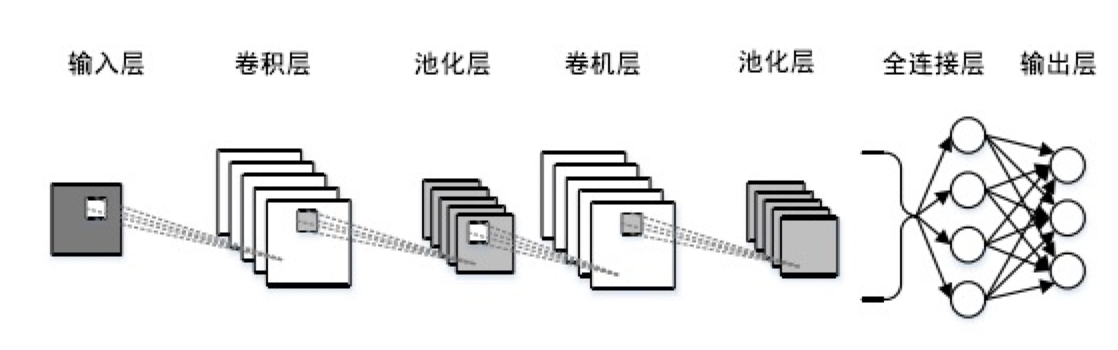
\includegraphics[scale=0.6]{fig2/C5/CNN结构}%联邦学习的系统架构
	\caption{卷积神经网络结构图}
  	\label{fig:卷积神经网络结构图} 
\end{figure}

CNN 网络中的损失函数为 nn.CrossEntropyLoss。该函数是nn.NLLLoss 和 nn.LogSoftmax 的结合,激活函数使用 Softmax 函数,损失函数使用交叉熵损失函数评估分类任务中的损失,也更便于计算反向传播算法。在选择梯度上传的全连接层与传输协议中, 部分超参数选择如下: 选择参数比例 $\theta_{u}=0.01$, 全局参数 $\theta_{d}$ 下载比例为 1 。为了允许在学习中更多的随机性, 将学习率设置为 $\alpha=1 \times 10^{-2}$, 学习速率衰减值为 $1 \times 10^{-7}$ 。参与者迭代过程使用表$\mathrm{CNN}$ 网络训练本地数据集,攻击者使用基于 CNN 网络的 DCGAN算法与成员推理攻击的白盒算法。实验在这样的参数设置下搭建一个包含 29 个正常参与者和 1 个攻击者的 分布式联邦学习系统, 30 个参与者(包含攻击者)都与中央参数服务器进行连接。

我们将与直接增加噪声的情况以及不加噪声的情况进行对比。实验中使用20000 条数据作为训练数据集,每一个客户端拥有 10 个样本的数据,剩下的样本则作为测试数据集,每种情况分别重复做 5 次并取平均值。实验通信迭代次数为T = 200,步长 α = 1e − 4 ,衰减系数 γ = 0.99。

\section{自适应扰动方案的实验评估}
针对第三章提出的自适应扰动框架,我们从模型预测的准确率和隐私预算参数$\epsilon$两个角度评估该方案,隐私预算参数越小,意味着隐私保护的力度越大;模型的准确率越高意味着模型的可用性越高。我们分别使用梯度固定加躁方法和梯度自适应加躁方法进行实验,实验结果如下。

(1)使用梯度固定加噪方法:使用所有公共训练集数据$D_{p u b}$进行计算,得到平均梯度0.001,将其作为固定的梯度裁剪阈值。
每轮迭代过程中,在训练批次大小L=600个样本中添加噪声,因此采样率为为$\mathrm{q}=\frac{L}{N}=\frac{600}{60000}=0.01$。在采集的训练样本中添加的噪声量为σ = 5,隐私参数为$\delta=10^{-5}$。如图\ref{fig:梯度固定加噪方法下模型准确率随隐私预算变化情况}所示,隐私预算参数ε为研究变量。随着隐私预算参数越大,差分隐私提供的隐私保护强度越小,噪声量越少,模型的准确率越高,符合理论原理。当隐私预算$\frac{\epsilon}{c}$≥ 5后,隐私预算参数对于模型准确率影响趋于平稳,综合来看,当$c$≥ 7后,部署了差分隐私机制的模型准确率能达到90$\%$左右,原始不加噪声的模型相比,准确率下降了7$\%$。
\begin{figure}[!hbt]
\centering
  	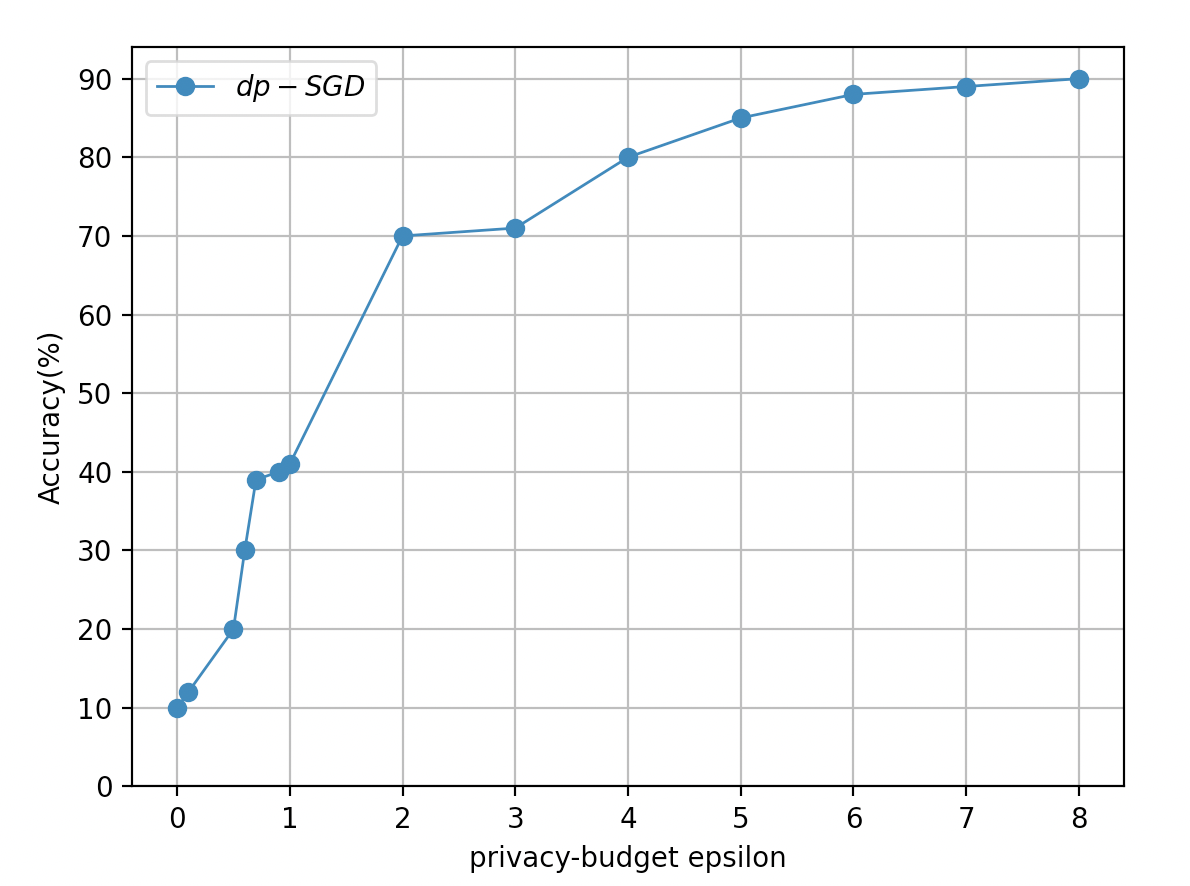
\includegraphics[scale=0.4]{fig2/C5/梯度固定}%联邦学习的系统架构
	\caption{梯度固定加噪方法下模型准确率随隐私预算变化情况}
  	\label{fig:梯度固定加噪方法下模型准确率随隐私预算变化情况} 
\end{figure}

(2)使用梯度自适应扰动方法:我们比较了在不同隐私预算下的自适应干扰模型的准确性,隐私预算分别为($\epsilon$1 = 0.1, $\epsilon$2 = 0.5, $\epsilon$3 = 2.0, $\epsilon$4 = 8.0)。
隐私预算$\epsilon$越小,噪音就越大。我们还为每个隐私预算选择三种不同的参数取值((a): f = 0.15, p = 0.85, (b): f = 0.10, p = 0.90(c): f = 0.05, p = 0.95)。可以肯定的是,设定的(f = 0.15, p = 0.85) 可以保证系统的隐私水平。在实验中,隐私预算ε的值是εc、εl和εc的总和。我们将隐私预算的计算分为以下三个步骤:对于贡献的计算、线性转换中的计算和
和损失函数的计算,即:$\epsilon_{c}=\epsilon_{l}=\epsilon_{f}=\frac{\epsilon}{3}$。

正如图\ref{fig:不同隐私预算的自适应干扰机制在MINIST数据集上的准确率}所示,随着隐私预算ε的增加,我们系统的准确性保持稳定的增长趋势。随着调整因子范围的不断缩小,自适应干扰模型的准确率逐渐降低,但仍保持较高的水平。例如,当隐私预算ε设置为8.0时,在f=0.15和p=0.85的设置下,APFL的准确率高达97.34$\%$,而在f=0.10和p=0.90的设置下,准确率为96.57$\%$,以及在f=0.05和p=0.95的设置下,准确率为96.25$\%$。

\begin{figure}[!hbt]
\centering
  	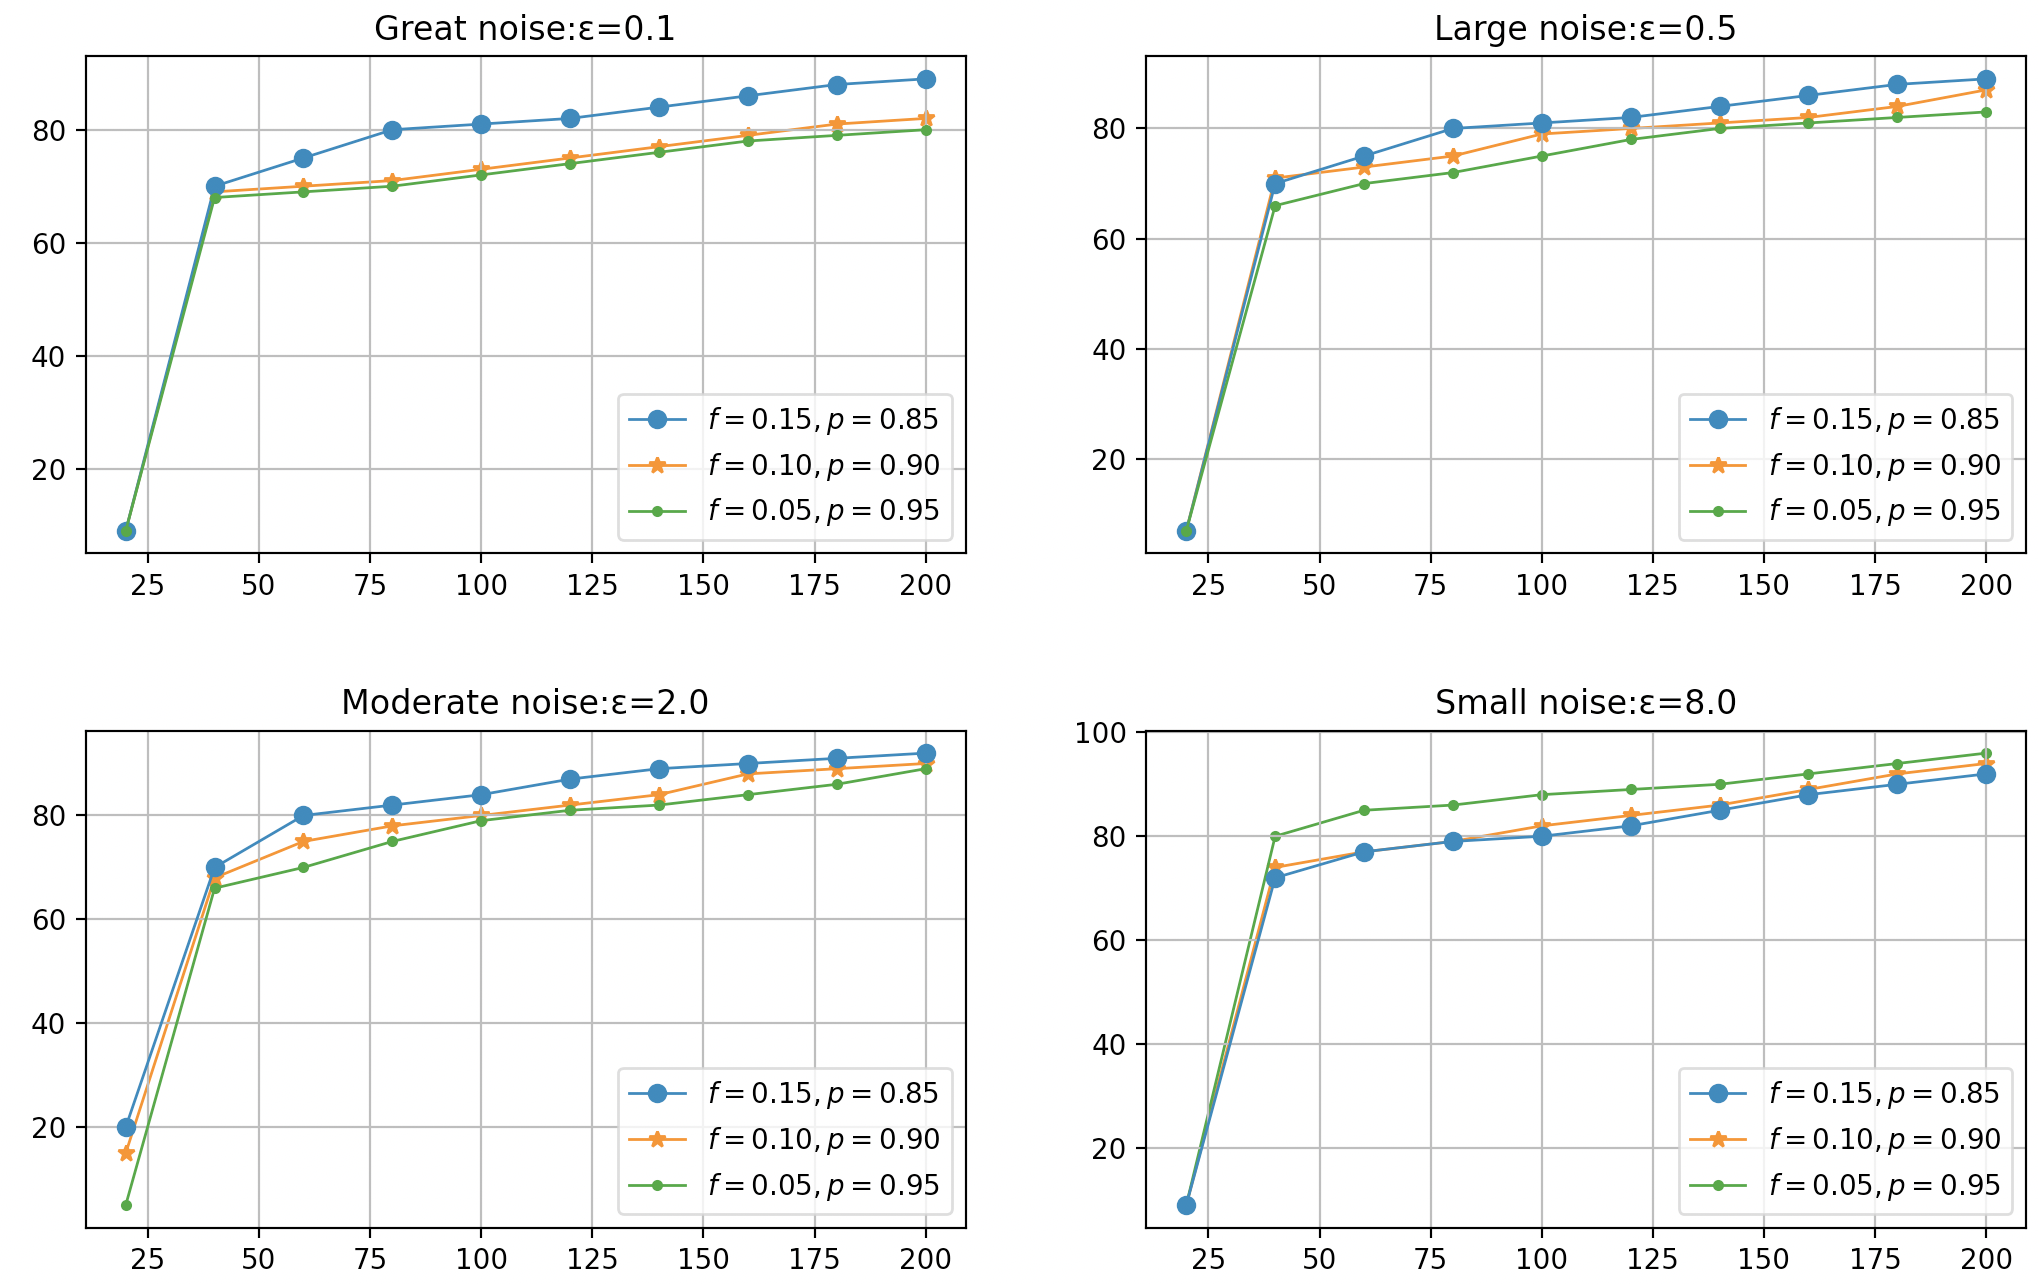
\includegraphics[scale=0.4]{fig2/C5/自适应干扰实验}%联邦学习的系统架构
	\caption{不同隐私预算的自适应干扰模型的准确率}
  	\label{fig:不同隐私预算的自适应干扰机制在MINIST数据集上的准确率} 
\end{figure}

综上,自适应隐私预算分配可以根据一般问题的收敛规律,合理地分配隐私参数,从而提高模型表现,但参数 γ 需要小心选取,过大的 γ 值会导致训练的初始阶段噪声太大,从而影响模型的可用性。

我们还与近年来使用DP机制保护深度学习模型隐私的工作进行了比较,如[1]中的DLPP和[18]中的DSSGD。在图\ref{fig:DP-SGD、DLPP、ACDP在模型准确率和隐私预算上的对比}中,我们可以清楚地得到一个信息,即我们的工作即使在强隐私保证下(ε=0.1)也表现良好。当调整因素设置为f = 0.15和p = 0.85时,模型的准确率在200个历时后达到88.46$\%$。此外,调整因素为f=0.05和p=0.95,自适应干扰模型的准确率为86.79$\%$。然而,在相同的隐私预算下,差分隐私随机梯度下降算法(DP-SGD)\upcite{ref45}的准确性仅达到79.63$\%$,本地差分隐私DLPP模型的准确性低于65.00$\%$。

\begin{figure}[!hbt]
\centering
  	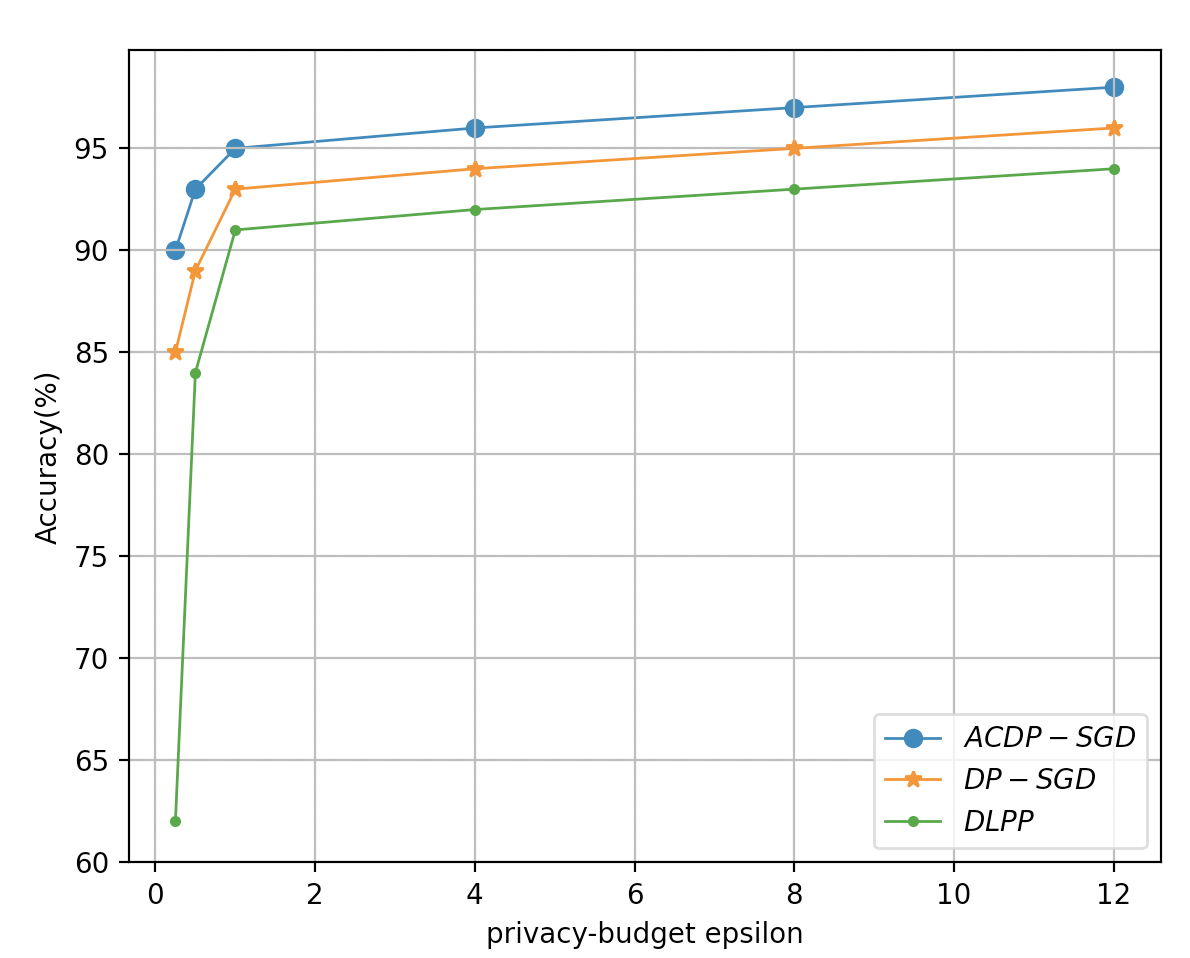
\includegraphics[scale=0.4]{fig2/C5/自适应干扰实验对比}%联邦学习的系统架构
	\caption{DP-SGD、DLPP、ACDP在模型准确率和隐私预算上的对比}
  	\label{fig:DP-SGD、DLPP、ACDP在模型准确率和隐私预算上的对比} 
\end{figure}


\section{安全混洗算法的实验评估}
我们在MNIST、FMNIST和CIFAR上评估所提出的安全聚合框架。为了评估参数:客户端数量$n$对于隐私预算和模型预测准确率的影响。如图\ref{fig:安全混洗模型中参与混洗的本地客户端数量对联合模型精度的影响}所示,通过客户端采样机制和梯度的拆分混洗算法,我们的安全混洗模型(下文简称SA-FL)能够以较低的隐私成本实现较高的准确性。在训练中增加客户数量n的同时,SA-FL的表现与无噪声的联合学习一样接近。与MNIST(n=100,ε=1)、FMNIST(n=200,ε=5)相比,CIFAR-10(n=500,ε=10)需要更多的客户端,这表明对于一个具有较大神经网络模型的更复杂的任务,当在更多的本地数据和更多的客户端上添加扰动之后,需要更多的通信回合才能使联合模型达到更高的精度。

\begin{figure}[!hbt]
\centering
  	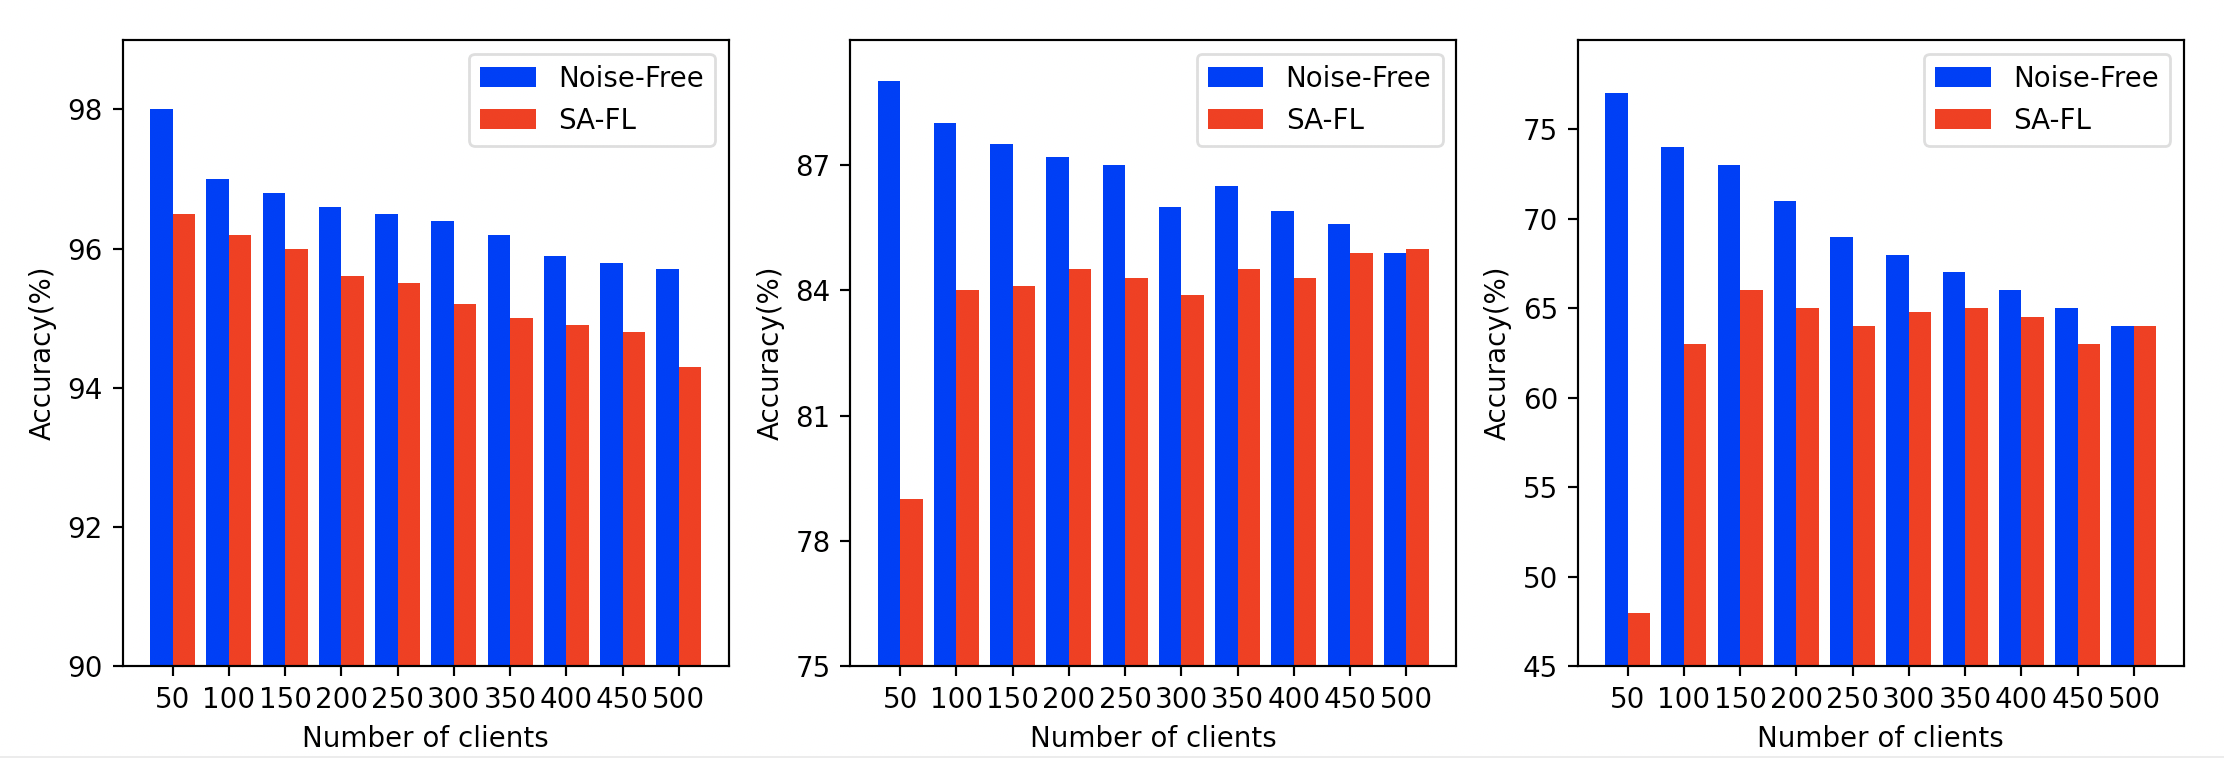
\includegraphics[scale=0.37]{fig2/C5/SA-FL}%联邦学习的系统架构
	\caption{安全混洗模型中参与混洗的本地客户端数量对联合模型精度的影响}
  	\label{fig:安全混洗模型中参与混洗的本地客户端数量对联合模型精度的影响} 
\end{figure}

接着,我们分别在MNIST, FMNIST and CIFAR-10评估了客户端采样比和通信回合对于模型训练准确率的影响。由图\ref{fig:安全混洗模型中通信轮数和客户端采样比对联合模型精度的影响}可以发现,当$f_{r}$太小的时候,并不影响在MNIST上的表现,但对FASHION-MNIST和CIFAR-10的表现影响很大。当$f_{r}$接近1时,安全聚合框架可以在MNIST、FASHION-MNIST和CIFAR-10上取得与无噪声结果几乎相同的性能。另一个重要的参数是中央参数聚合器和本地客户端之间的通信轮次$m$。不难看出,随着通信次数的增加,我们可以通过所提出的模型在所有数据集上训练出更好的模型。然而,由于数据和任务的复杂性,CIFAR-10需要更多的通信回合以获得更好的模型。

\begin{figure}[!hbt]
\centering
  	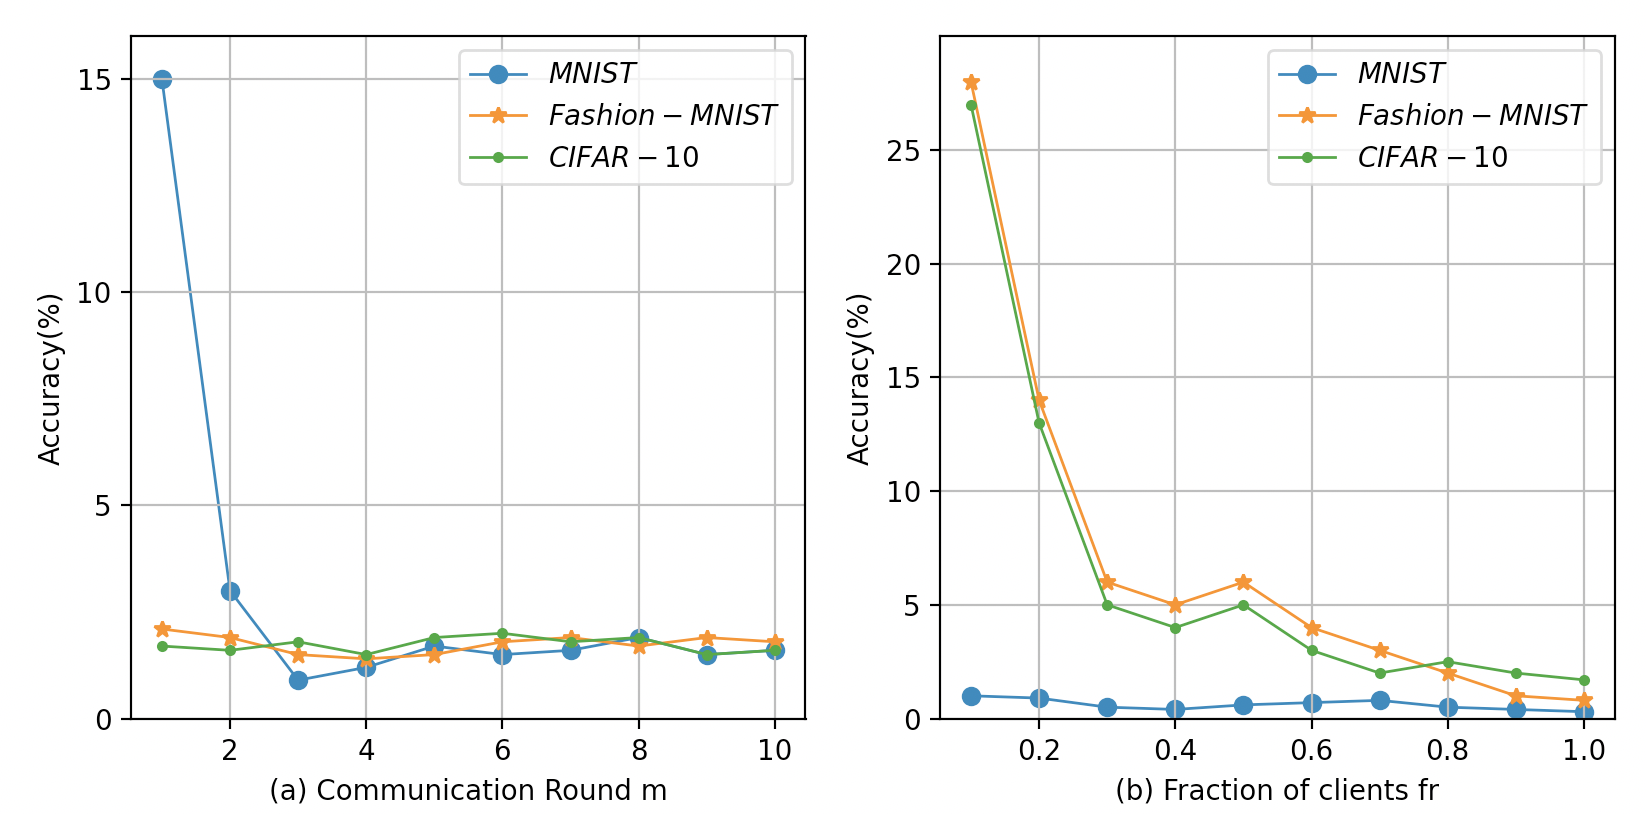
\includegraphics[scale=0.4]{fig2/C5/SA-FL2}%联邦学习的系统架构
	\caption{安全混洗模型中通信轮数和客户端采样比对联合模型精度的影响}
  	\label{fig:安全混洗模型中通信轮数和客户端采样比对联合模型精度的影响} 
\end{figure}

最后,我们将统一比较应用了自适应差分隐私算法和安全混洗器的联邦学习模型与其他联邦学习隐私保护模型,在相同隐私预算参数下训练模型能达到的精度。如图\ref{自适应差分混洗模型和其他联邦学习隐私保护模型的比较}(a-c)中,SA-FL在ε=4和n=100的情况下可以达到96.24$\%$的准确率,在ε=4,n=200的情况下可以达到86.26$\%$的准确率,在ε=10,n=500的情况下,在MNIST,FMNIST和CIFAR-10上可以达到61.4$\%$的准确率。我们的结果与之前的其他工作相比非常有竞争力。[Geyer等人,2017]首次将差分隐私应用于联邦学习,虽然他们只使用了100个客户端,但在MNIST上,他们只能在(ε,m)=(8,11),(8,54)和(8,412)的情况下达到78$\%$,92$\%$和96$\%$的准确率,其中(ε,m)代表隐私预算和通信回合。[Bhowmick等人,2018]首次在联合学习中利用本地差分隐私。由于其机制的高变异性,它需要超过200轮的通信,并花费更多的隐私预算,即MNIST(ε=500)和CIFAR-10(ε=5000)。最近的工作[Truex等人,2020]将压缩后的局部差分隐私(α-CLDP)应用到联邦学习中,在FMNIST数据集上获得了86.93$\%$的准确性。然而,α-CLDP需要相对较大的隐私预算ε = α-2c-10ρ(例如,α = 1,c = 1,ρ = 10)来实现该性能,这导致了较弱的隐私保证。与以往的工作相比,我们的方法在客户端和云端之间需要更少的通信回合(例如,MNIST为10,FMNIST和CIFAR-10为15),这使得整个解决方案在实际场景中更加实用。总的来说,SA-FL在隐私成本、模型精度和通信成本方面都比之前的作品取得了更好的表现。

\begin{figure}[!hbt]
\centering
  	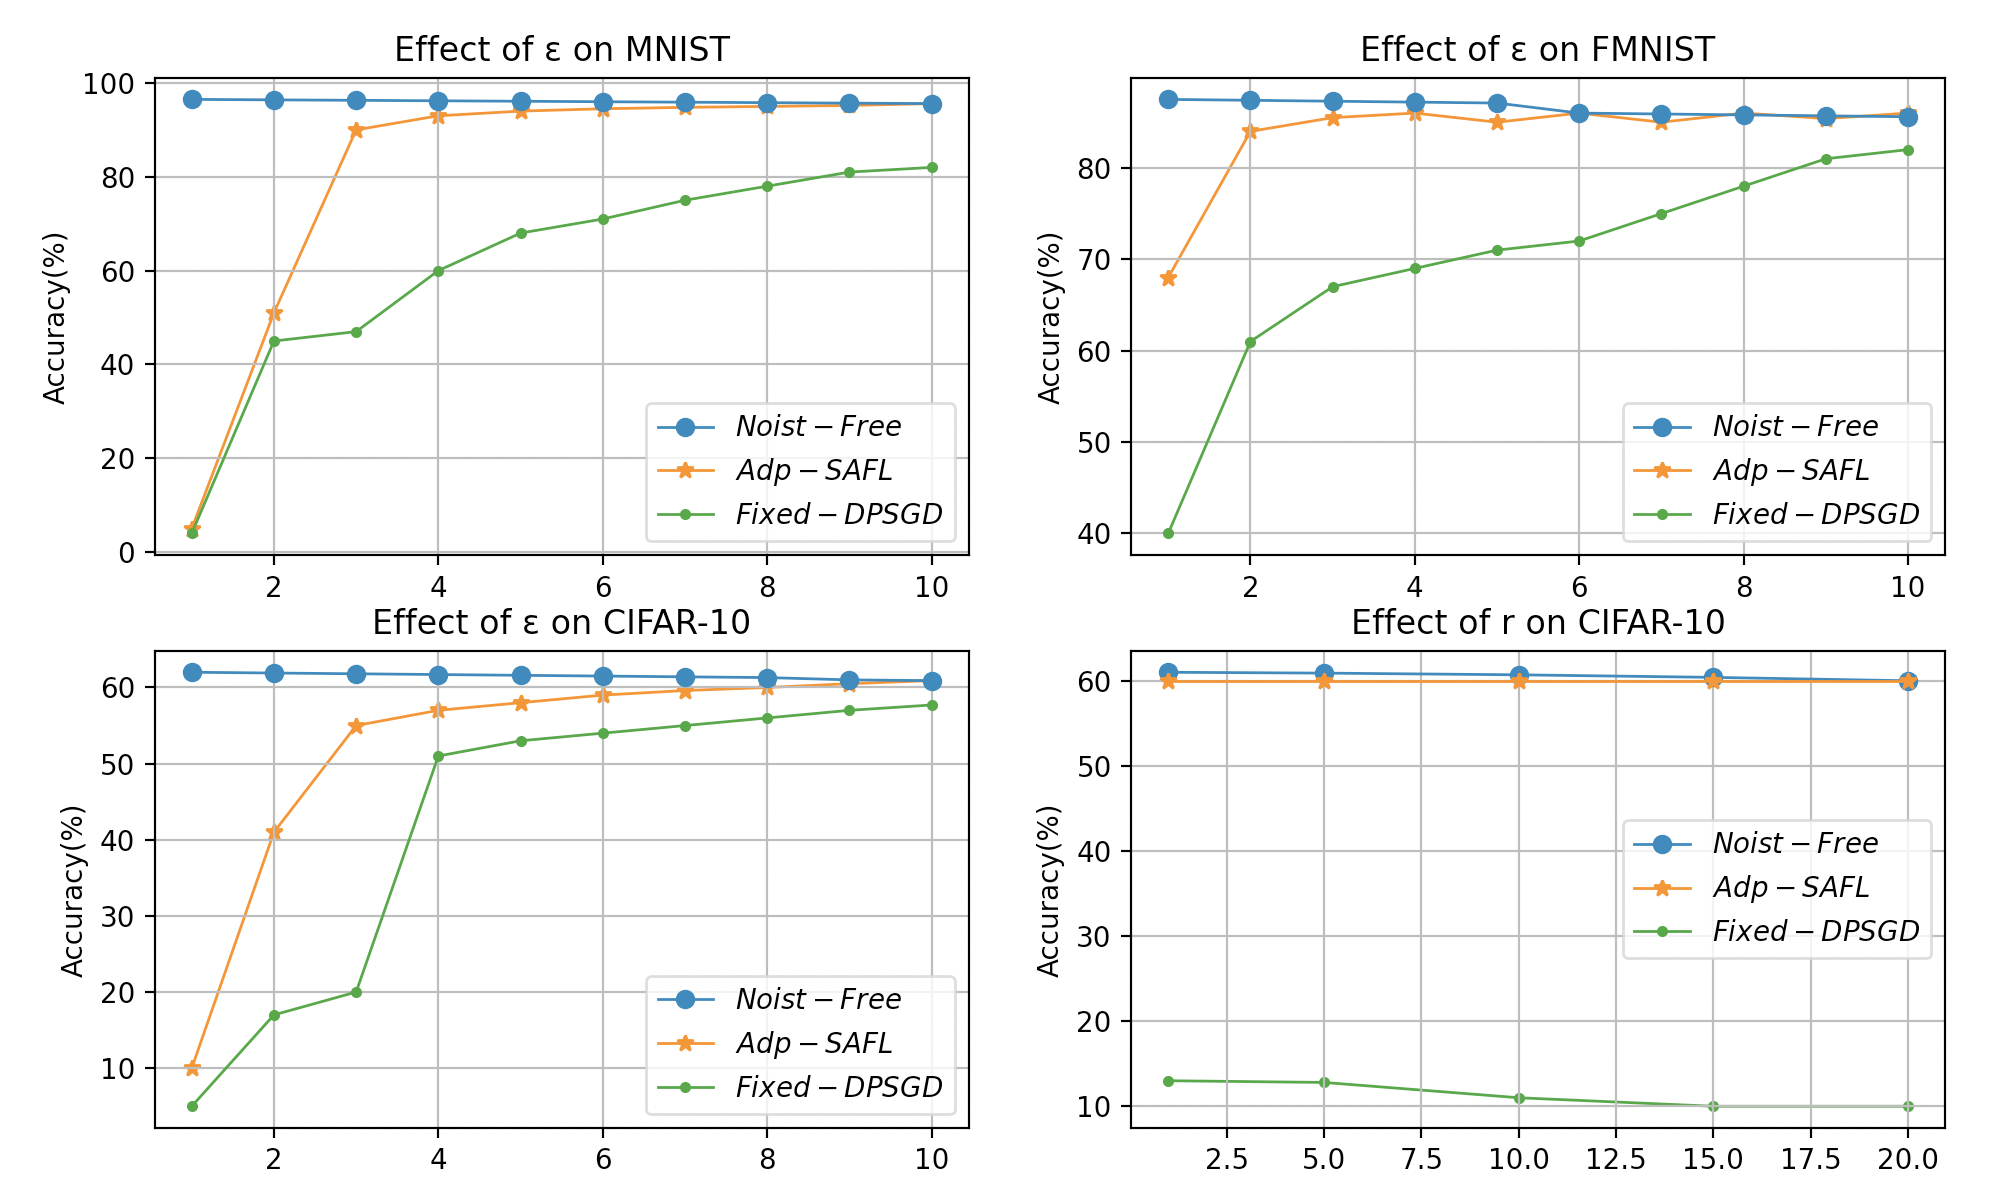
\includegraphics[scale=0.4]{fig2/C5/SA-FL对比实验}%联邦学习的系统架构
	\caption{自适应差分混洗模型和其他联邦学习隐私保护模型的比较}
  	\label{自适应差分混洗模型和其他联邦学习隐私保护模型的比较} 
\end{figure}

\section{结果分析}
为了验证自适应扰动算法对于模型训练的精度也能维持在较优的水平,我们进行了对比实验,使用自适应扰动算法和不使用这种方法在不同的隐私参数$\epsilon$下的对比实验。由本章第三节对于自适应差分隐私方案的实验评估,我们可以看到自适应
扰动算法基本上占有绝对的优势,尤其是在损失函数值,在隐私参数$\epsilon$=0.1时,我们的方法不到1,而传统的平均算法却在100左右。这么大的差距的原因在于,自适应扰动算法的权重分配使得聚合时个体信噪比不变,但整体的聚合结果的信噪比却提高了很多,因此当隐私参数$\epsilon$很小,即噪声量很大的时候,表现越好。而当$\epsilon$越大时,注入的噪声也就越小,自适应加躁方法的效果就没有噪声大的时候明显.

系统的额外开销主要来自服务器端的预训练过程,以及用户端在开始训练前对贡献的计算和扰动。我们使用20个历时来训练云服务器的初始化网络,这平均需要68.22秒。在独立和异步的训练过程之前,用户需要用层间依赖传播算法计算权重。这个过程只需要训练正向传播过程,而不需要计算反向传播过程中的梯度和损失惩罚。其平均时间为4.35毫秒。
为了减轻隐私威胁,我们的解决方案是向权重、线性变换函数中的原始数据和损失函数的系数注入拉普拉斯噪声。向权重注入噪声的步骤可以与计算贡献同步进行,这需要额外的2.67毫秒时间。向线性变换中的原始数据和损失函数的系数注入自适应噪声的操作可以在训练前完成,每一个历时的计算都与扰动的权重相似。因此,在模型效率方面的提升是非常突出的。

从隐私成本和模型精度的总体上看,混洗差分隐私方法在各统计问题的结果可用性上都有着相比本地化差分隐私方法明显更优的结果。但从通信代价和计算代价的角度分析,安全混洗算法中混洗器的引入,一方面使得用户数据与用户所使用的编码器之间的关联性消失,使得分析器端的计算代价增大;另一方面造成了分析器端的通信代价增大。如何兼顾数据的隐私性、可用性、算法的计算代价和通信代价是后续基于SA-FL框架构建的隐私保护方法需加以研究的部分。


\section{本章小结}
在本章中,我们选取了三个基准数据集对本文提出的自适应本地差分隐私和安全混洗框架进行了一系列的实验来测试其可行性,并且在联邦学习系统上也进行实验和研究。实验结果表明,我们的自适应本地差分隐私可以有效降低隐私预算,并且维持模型精度。安全混洗框架能通过客户端采样算法和梯度的拆分混洗算法,降低隐私保护预算,提高数据的可用性。


\chapter{总结与展望}
\label{ch6}
\section{总结}
随着深度学习的兴起,出现了越来越多新的模型和算法,能够更有效的解决各类问题。基于人工智能的产品也在各个领域迎来了一波新的发展热潮,给人民的生活带来了巨大的便利。然而用户在享受深度学习模型带来便利的同时,必须共享自己的数据,随着隐私泄露事件越来越多,数据的安全和隐私问题也逐步引起了人们的关注。 

与此同时,各类智能设备也在不断发展,用户产生的数据也越来越多,智能设备的算力不断增强。用户不愿意向商业公司或商业机构提供个人隐私数据。分布式联邦学习系统解决分布式终端用户在本地更新模型的问题,联邦学习的目标是保障大数据共享信息时的数据安全、保护本地数据和个人隐私,在多计算节点之间高效的训练机器学习模型。 

分布式联邦学习系统得到了广泛的研究和应用,成为传统集中式机器学习方法的一种改进方法。它不是将数据上传到中心服务器进行集中训练,而是参与者在本地进行模型训练并与参数服务器共享模型更新。参数服务器对来自多个参与者的权重进行聚合,并组合创建一个改进的全局模型,这有助于保障用户的数据隐私和降低通信成本。 

本文主要研究针对分布式联邦学习系统的隐私安全问题。通过研究分布式联邦深度学习的系统漏洞,提出了一套分布式联邦系统中针对攻击的隐私安全方案对策。本文的主要工作和贡献如下:
\begin{enumerate}
\item [(1)] 基于本地差分隐私的权重分配自适应干扰算法。在客户端本地训练的神经网络模型中,通过分析前向传播算法,计算每个属性类对于模型输出的贡献比,然后,我们开发了一个自适应噪声添加的方案,根据贡献率注入不同隐私预算的噪声。与传统的注入噪声的方法相比,我们在相同的隐私保护程度下最大限度地提高了模型的准确性,减少噪声对模型输出结果的影响,提高模型精度。而且,本文也从本地差分隐私定义的角度,理论证明了提出的方法满足$\mathcal{E}$-本地差分隐私.最后通过多组真实数据集以及合成数据集验证了本地自适应扰动机制的性能,证明了其在相同条件下要优于现有的同类方法。

\item [(2)] 本文提出了SA安全混洗框架,混洗差分隐私摒弃了中心化差分隐私下对可信第三方的依赖,即无需任何可信第三方。对用户的原始数据进行统一的扰动处理,提高了隐私性;弥补了中心化差分隐私与本地化差分隐私在可用性上约O( n) 的间隙,在差分隐私的保证下实现了数据隐私度与可用性之间的更好平衡。
\end{enumerate}

综上所述,本文的研究充分证明了所提出框架的有效性,可以极大的联邦学习模型的隐私性和可用性,从而进一步推进了联邦学习在安全领域的应用和发展。

\section{展望}
在可预见的未来,大规模、大数据、分布式的深度学习将得到快速发展。5G、边缘计算、物联网等技术也将迅速普及。人类将彻底步入人工智能时代。在此我将对我未来的研究做出几点展望:
\begin{enumerate}
\item [(1)] 本文提出的自适应的差分隐私深度学习算法是一种基础算法,它可以令学习模型在训练过程中总体隐私不累加。因此后续可以研究其在大型数据集与复杂模型结构中的表现。 
\item [(2)] 现实中,分布式协作学习可能由极多的参与者组成,如百万部手机等。同时分布式协作学习中的每个设备可能计算、通信和存储能力等都有很大不同。因此有关实际应用中的通信、异构问题等也需要进行大量的研究。 
\item[(3)] 分布式协作学习需要一个公平的平台和激励机制,可以在实际应用中明显体现出效果提升,并能够在永久数据记录机制(如区块链等)中留下记录。这样才能促进分布式协作学习的商业化与大规模应用。
\end{enumerate}


%\appendix

\chapter{模型示例}
\label{ch7}
% \section{SCADE文本模型}

\linespread{1}

% \lstinputlisting[language=Caml, caption=SCADE文本模型示例]{fig/7/scade.scade}

\section{NuSMV目标模型}

\lstinputlisting[language=VHDL, caption=NuSMV目标模型示例-子状态机模块]{fig/7/nusmv1.smv}

\lstinputlisting[language=VHDL, caption=NuSMV目标模型示例-监控变量模块]{fig/7/nusmv2.smv}

\lstinputlisting[language=VHDL, caption=NuSMV目标模型示例-自定义函数节点模块]{fig/7/nusmv3.smv}

\lstinputlisting[language=VHDL, caption=NuSMV目标模型示例-顶层主函数模块]{fig/7/nusmv4.smv}






\pagestyle{plain}
\clearpage
\phantomsection
\addcontentsline{toc}{chapter}{参考文献}
\bibliographystyle{gbt7714-2005}
\bibliography{bib/tex}

\begin{thebibliography}{99}

\bibitem{ref1}Pouyanfar S, Sadiq S, Yan Y, et al. A survey on deep learning: Algorithms, techniques, and applications[J]. ACM Computing Surveys (CSUR), 2018, 51(5): 1-36.
\bibitem{ref2}Voigt P, Von dem Bussche A. The eu general data protection regulation (gdpr)[J]. A Practical Guide, 1st Ed., Cham: Springer International Publishing, 2017, 10: 3152676.
\bibitem{ref3}Bonawitz K, Ivanov V, Kreuter B, et al. Practical secure aggregation for privacy-preserving machine learning[C]//proceedings of the 2017 ACM SIGSAC Conference on Computer and Communications Security. 2017: 1175-1191.
\bibitem{ref4}Hu R, Dollár P, He K, et al. Learning to segment every thing[C]//Proceedings of the IEEE Conference on Computer Vision and Pattern Recognition. 2018: 4233-4241.
\bibitem{ref5}张仕良. 基于深度神经网络的语音识别模型研究[D]. 合肥: 中国科学技术大学, 2017.
\bibitem{ref6}Sardianos C, Tsirakis N, Varlamis I. A survey on the scalability of recommender systems for social networks[M]//Social Networks Science: Design, Implementation, Security, and Challenges. Springer, Cham, 2018: 89-110.
\bibitem{ref7}Shen D, Wu G, Suk H I. Deep learning in medical image analysis[J]. Annual review of biomedical engineering, 2017, 19: 221-248.
\bibitem{ref8}Papernot N, Abadi M, Erlingsson U, et al. Semi-supervised knowledge transfer for deep learning from private training data[J]. arXiv preprint arXiv:1610.05755, 2016.
\bibitem{ref9}Dwork C, McSherry F, Nissim K, et al. Calibrating noise to sensitivity in private data analysis[C]//Theory of cryptography conference. Springer, Berlin, Heidelberg, 2006: 265-284.
\bibitem{ref10}Rivest R L, Adleman L, Dertouzos M L. On data banks and privacy homomorphisms[J]. Foundations of secure computation, 1978, 4(11): 169-180.
\bibitem{ref11}Wu X, Fredrikson M, Jha S, et al. A methodology for formalizing model-inversion attacks[C]//2016 IEEE 29th Computer Security Foundations Symposium (CSF). IEEE, 2016: 355-370.
\bibitem{ref12}Hitaj B, Ateniese G, Perez-Cruz F. Deep models under the GAN: information leakage from collaborative deep learning[C]//Proceedings of the 2017 ACM SIGSAC Conference on Computer and Communications Security. 2017: 603-618.
\bibitem{ref13}Shokri R, Stronati M, Song C, et al. Membership inference attacks against machine learning models[C]//2017 IEEE Symposium on Security and Privacy (SP). IEEE, 2017: 3-18.
\bibitem{ref14}Dwork C. Differential privacy[C]//International Colloquium on Automata, Languages, and Programming. Springer, Berlin, Heidelberg, 2006: 1-12.
\bibitem{ref15}Alfeld S, Zhu X, Barford P. Data poisoning attacks against autoregressive models[C]//Proceedings of the AAAI Conference on Artificial Intelligence. 2016, 30(1).
\bibitem{ref16}Yao A C. Protocols for secure computations[C]//23rd annual symposium on foundations of computer science (sfcs 1982). IEEE, 1982: 160-164.
\bibitem{ref17}Meng X, Bradley J, Yavuz B, et al. Mllib: Machine learning in apache spark[J]. The Journal of Machine Learning Research, 2016, 17(1): 1235-1241.
\bibitem{ref18}Wang X, Han Y, Wang C, et al. In-edge ai: Intelligentizing mobile edge computing, caching and communication by federated learning[J]. IEEE Network, 2019, 33(5): 156-165.
\bibitem{ref19}Li T, Sahu A K, Talwalkar A, et al. Federated learning: Challenges, methods, and future directions[J]. IEEE Signal Processing Magazine, 2020, 37(3): 50-60.
\bibitem{ref20}Tran N H, Bao W, Zomaya A, et al. Federated learning over wireless networks: Optimization model design and analysis[C]//IEEE INFOCOM 2019-IEEE Conference on Computer Communications. IEEE, 2019: 1387-1395.
\bibitem{ref21}McMahan B, Moore E, Ramage D, et al. Communication-efficient learning of deep networks from decentralized data[C]//Artificial intelligence and statistics. PMLR, 2017: 1273-1282.
\bibitem{ref22}Zhu L, Han S. Deep leakage from gradients[M]//Federated learning. Springer, Cham, 2020: 17-31.
\bibitem{ref23}Aono Y, Hayashi T, Wang L, et al. Privacy-preserving deep learning via additively homomorphic encryption[J]. IEEE Transactions on Information Forensics and Security, 2017, 13(5): 1333-1345.
\bibitem{ref24}Ma C, Li J, Ding M, et al. On safeguarding privacy and security in the framework of federated learning[J]. IEEE network, 2020, 34(4): 242-248.
\bibitem{ref25}曹志义, 牛少彰, 张继威. 基于半监督学习生成对抗网络的人脸还原算法研究[J]. 电子与信息学报, 2018, 40(2): 323-330. Distributed differ- ential privacy via shuffling. In Eurocrypt. Springer, 2019.
\bibitem{ref26}Goodfellow I, Pouget-Abadie J, Mirza M, et al. Generative adversarial nets[J]. Advances in neural information processing systems, 2014, 27.
\bibitem{ref27}Radford A, Metz L, Chintala S. Unsupervised representation learning with deep convolutional generative adversarial networks[J]. arXiv preprint arXiv:1511.06434, 2015.
\bibitem{ref28}Salimans T, Goodfellow I, Zaremba W, et al. Improved techniques for training gans[J]. Advances in neural information processing systems, 2016, 29: 2234-2242.
\bibitem{ref29}Goodfellow I, Bengio Y, Courville A. Deep learning[M]. MIT press, 2016.
\bibitem{ref30}Johnson R, Zhang T. Accelerating stochastic gradient descent using predictive variance reduction[J]. Advances in neural information processing systems, 2013, 26: 315-323.
\bibitem{ref31}Zhang T. Solving large scale linear prediction problems using stochastic gradient descent algorithms[C]//Proceedings of the twenty-first international conference on Machine learning. 2004: 116.
\bibitem{ref32}Dwork C, Kenthapadi K, McSherry F, et al. Our data, ourselves: Privacy via distributed noise generation[C]//Annual International Conference on the Theory and Applications of Cryptographic Techniques. Springer, Berlin, Heidelberg, 2006: 486-503.
\bibitem{ref33}McSherry F, Talwar K. Mechanism design via differential privacy[C]//48th Annual IEEE Symposium on Foundations of Computer Science (FOCS'07). IEEE, 2007: 94-103.
\bibitem{ref34}LBengio Y. Learning deep architectures for AI[M]. Now Publishers Inc, 2009.
\bibitem{ref35}Dwork C, Roth A. The algorithmic foundations of differential privacy[J]. Found. Trends Theor. Comput. Sci., 2014, 9(3-4): 211-407.
\bibitem{ref36}Bassily R, Smith A, Thakurta A. Private empirical risk minimization: Efficient algorithms and tight error bounds[C]//2014 IEEE 55th Annual Symposium on Foundations of Computer Science. IEEE, 2014: 464-473.
\bibitem{ref37}Acs G, Melis L, Castelluccia C, et al. Differentially private mixture of generative neural networks[J]. IEEE Transactions on Knowledge and Data Engineering, 2018, 31(6): 1109-1121.
\bibitem{ref38}Su D, Cao J, Li N, et al. Differentially private k-means clustering and a hybrid approach to private optimization[J]. ACM Transactions on Privacy and Security (TOPS), 2017, 20(4): 1-33.
\bibitem{ref39}Salakhutdinov R, Mnih A, Hinton G. Restricted Boltzmann machines for collaborative filtering[C]//Proceedings of the 24th international conference on Machine learning. 2007: 791-798.
\bibitem{ref40}Bassily R, Smith A, Thakurta A. Private empirical risk minimization: Efficient algorithms and tight error bounds[C]//2014 IEEE 55th Annual Symposium on Foundations of Computer Science. IEEE, 2014: 464-473.
\bibitem{ref41}McSherry F D. Privacy integrated queries: an extensible platform for privacy-preserving data analysis[C]//Proceedings of the 2009 ACM SIGMOD International Conference on Management of data. 2009: 19-30.
\bibitem{ref42}Thakurta A G. Differentially private convex optimization for empirical risk minimization and high-dimensional regression[M]. The Pennsylvania State University, 2013.
\bibitem{ref43}Lee J, Kifer D. Concentrated differentially private gradient descent with adaptive per-iteration privacy budget[C]//Proceedings of the 24th ACM SIGKDD International Conference on Knowledge Discovery Data Mining. 2018: 1656-1665.
\bibitem{ref44}Balle B, Wang Y X. Improving the Gaussian mechanism for differential privacy: Analytical calibration and optimal denoising[C]//International Conference on Machine Learning. PMLR, 2018: 394-403.
\bibitem{ref45}Shokri R, Shmatikov V. Privacy-preserving deep learning[C]//Proceedings of the 22nd ACM SIGSAC conference on computer and communications security. 2015: 1310-1321.
\bibitem{ref46}LeCun Y, Bottou L, Bengio Y, et al. Gradient-based learning applied to document recognition[J]. Proceedings of the IEEE, 1998, 86(11): 2278-2324.
\bibitem{ref47}Song S, Chaudhuri K, Sarwate A D. Stochastic gradient descent with differentially private updates[C]//2013 IEEE Global Conference on Signal and Information Processing. IEEE, 2013: 245-248.
\bibitem{ref48}Geyer R C, Klein T, Nabi M. Differentially private federated learning: A client level perspective[J]. arXiv preprint arXiv:1712.07557, 2017.
\bibitem{ref49}Truex S, Baracaldo N, Anwar A, et al. A hybrid approach to privacy-preserving federated learning[C]//Proceedings of the 12th ACM Workshop on Artificial Intelligence and Security. 2019: 1-11.
\bibitem{ref50}Nesterov Y. Introductory lectures on convex optimization: A basic course[M]. Springer Science Business Media, 2003.
\bibitem{ref51}  M, Lantz E, Jha S, et al. Privacy in pharmacogenetics: An end-to-end case study of personalized warfarin dosing[C]//23rd {USENIX} Security Symposium ({USENIX} Security 14). 2014: 17-32.
\bibitem{ref52}McMahan H B, Ramage D, Talwar K, et al. Learning differentially private recurrent language models[J]. arXiv preprint arXiv:1710.06963, 2017.
\bibitem{ref53}Geyer R C, Klein T, Nabi M. Differentially private federated learning: A client level perspective[J]. arXiv preprint arXiv:1712.07557, 2017.
\bibitem{ref54}Bhowmick A, Duchi J, Freudiger J, et al. Protection against reconstruction and its applications in private federated learning[J]. arXiv preprint arXiv:1812.00984, 2018.
\bibitem{ref55}Truex S, Liu L, Chow K H, et al. LDP-Fed: Federated learning with local differential privacy[C]//Proceedings of the Third ACM International Workshop on Edge Systems, Analytics and Networking. 2020: 61-66.
\bibitem{ref56}Comiter M. Attacking artificial intelligence[J]. Belfer Center Paper, 2019: 2019-08.
\bibitem{ref57}Abadi M, Chu A, Goodfellow I, et al. Deep learning with differential privacy[C]//Proceedings of the 2016 ACM SIGSAC conference on computer and communications security. 2016: 308-318.
\bibitem{ref58}Papernot N, Abadi M, Erlingsson U, et al. Semi-supervised knowledge transfer for deep learning from private training data[J]. arXiv preprint arXiv:1610.05755, 2016.
\bibitem{ref59}Xie L, Lin K, Wang S, et al. Differentially private generative adversarial network[J]. arXiv preprint arXiv:1802.06739, 2018.
\bibitem{ref60}Jordon J, Yoon J, Van Der Schaar M. PATE-GAN: Generating synthetic data with differential privacy guarantees[C]//International conference on learning representations. 2018.
\bibitem{ref61}Zhang J, Zheng K, Mou W, et al. Efficient private ERM for smooth objectives[J]. arXiv preprint arXiv:1703.09947, 2017.
\bibitem{ref62}Wang D, Ye M, Xu J. Differentially private empirical risk minimization revisited: Faster and more general[J]. arXiv preprint arXiv:1802.05251, 2018.
\bibitem{ref63}Wang D, Chen C, Xu J. Differentially private empirical risk minimization with non-convex loss functions[C]//International Conference on Machine Learning. PMLR, 2019: 6526-6535.
\bibitem{ref64}Abadi M, Chu A, Goodfellow I, et al. Deep learning with differential privacy[C]//Proceedings of the 2016 ACM SIGSAC conference on computer and communications security. 2016: 308-318.
\bibitem{ref65}Bach S, Binder A, Montavon G, et al. On pixel-wise explanations for non-linear classifier decisions by layer-wise relevance propagation[J]. PloS one, 2015, 10(7): e0130140.
\bibitem{ref66}Sashank J Reddi, Ahmed Hefny, Suvrit Sra, Barnabas Poczos, and Alex Smola. Stochastic variance reduction for nonconvex optimization. In International conference on machine learning, pages 314–323, 2016.
\bibitem{ref68}Krizhevsky A, Hinton G. Learning multiple layers of features from tiny images[J]. 2009.
\bibitem{ref69}Melis L, Song C, De Cristofaro E, et al. Exploiting unintended feature leakage in collaborative learning[C]//2019 IEEE Symposium on Security and Privacy (SP). IEEE, 2019: 691-706.
\bibitem{ref70}Shokri R, Stronati M, Song C, et al. Membership inference attacks against machine learning models[C]//2017 IEEE Symposium on Security and Privacy (SP). IEEE, 2017: 3-18.
\bibitem{ref71}Bonawitz K, Ivanov V, Kreuter B, et al. Practical secure aggregation for privacy-preserving machine learning[C]//proceedings of the 2017 ACM SIGSAC Conference on Computer and Communications Security. 2017: 1175-1191.
\bibitem{ref72}Balle B, Bell J, Gascón A, et al. The privacy blanket of the shuffle model[C]//Annual International Cryptology Conference. Springer, Cham, 2019: 638-667.
\bibitem{ref73}Young T, Hazarika D, Poria S, et al. Recent trends in deep learning based natural language processing[J]. ieee Computational intelligenCe magazine, 2018, 13(3): 55-75.
\bibitem{ref75}Dwork C. A firm foundation for private data analysis[J]. Communications of the ACM, 2011, 54(1): 86-95.
\bibitem{ref76}Bach S, Binder A, Montavon G, et al. On pixel-wise explanations for non-linear classifier decisions by layer-wise relevance propagation[J]. PloS one, 2015, 10(7): e0130140.
\bibitem{ref77}Binder A, Montavon G, Lapuschkin S, et al. Layer-wise relevance propagation for neural networks with local renormalization layers[C]//International Conference on Artificial Neural Networks. Springer, Cham, 2016: 63-71.
\bibitem{ref78}Aji A F, Heafield K. Sparse communication for distributed gradient descent[J]. arXiv preprint arXiv:1704.05021, 2017.
\bibitem{ref79}Choudhury O, Gkoulalas-Divanis A, Salonidis T, et al. Differential privacy-enabled federated learning for sensitive health data[J]. arXiv preprint arXiv:1910.02578, 2019.
\bibitem{ref80}Wei K, Li J, Ding M, et al. Federated learning with differential privacy: Algorithms and performance analysis[J]. IEEE Transactions on Information Forensics and Security, 2020, 15: 3454-3469.

\end{thebibliography}


% \pagestyle{plain}
% \clearpage
% \phantomsection
% \addcontentsline{toc}{chapter}{致谢}
% {\fangsong
	\chapter*{致\qquad 谢}\vskip 2mm
	\vspace{-1cm}
		\large{

时光荏苒,岁月如梭,研究生的日子过得飞快,转眼间我的硕士研究生学习生涯即将接近尾声。在华东师范大学读研的这两年时光,我不但学习到了很多知识,也结识了许多良师益友,此时此刻,我的内心充满了无限的感慨。所谓饮水思源,在此我要向每位陪伴我,鼓励我,教导我的人表示由衷的感谢。

从2019年收到华东师范大学的研究生录取通知书,我满怀憧憬和抱负的来到华师大,来到上海可信计算实验室,有幸成为曹珍富老师的学生。
感谢实验室的各位老师们,他们不但为我们提供了优质的教学环境和资源,还创造了良好的学习氛围,通过一流的科研实力和丰富的科研热情带领我们学习最前沿的科研成果。为了充实我们的研究生生活,学院定期举办各种学术会议和活动,邀请到国内外知名学者给我们做讲座,让我们有机会接触到最新的科研成果。而且,无论是在科研还是生活上遇到问题,老师们都会耐心的给我们提建议,鼓励帮助我们一起克服这些困难。

研究生的时光是轻快而稍纵即逝的,和实验室同学、室友的朝夕相处是我最难忘的回忆。因为有室友高圆圆、陈少敏、冯世玲,宿舍的氛围一直是欢快的,我们早晨共同早起去图书馆自习,下课了去实验室读论文,空闲时间一起在操场打篮球,欢声笑语,常伴我们。三年时光里,我们彻夜未睡,通宵准备数模竞赛;早出晚归,一起在理科楼度过日日夜夜,都将成为我的学生时代美好的回忆。

同门情谊似手足之情,感谢实验室的各位同窗好友,吴楠、汤琦、陆鹏皓、李翔宇、任城东、李明冲等,是有你们的互励互助,我才得以开心努力而充实的度过了这段美好的研究生生活,希望以后仍然有机会共同努力、共同奋斗。

最后,非常感谢我的父母和家人一直以来对我的鼓励与陪伴。在研究生生涯的这两年,我更加深刻体会到未来自己身上所担负的责任,希望我在未来的工作中能兢兢业业,踏实负责,实现我的社会价值;在未来的生活中,希望我能多多陪伴我的父母以回报养育之恩。 

在这篇论文完成之际意味着三年的硕士生涯即将告一段落,而自己也将踏上人生的下一段旅程。回顾硕士三年的时光,非常有幸能成为华东师范大学的学子。非常庆幸能成为曹珍富老师的学生,非常庆幸能和实验室的大家成为朋友,这是人生中可与而不可求的经历。最后,也感谢各位评审和答辩的专家在百忙之中对我论文的指导,谢谢你们。
	}
	
	\vspace{0.2cm}
	
	\vspace{0.2cm} \hspace{9.8cm}
	何慧娴
	
	\hspace{9cm}  二零二壹年九月

} 

% \pagestyle{plain}
% \clearpage
% \phantomsection
% \addcontentsline{toc}{chapter}{发表论文和科研情况}
% \chapter*{\large 攻读硕士学位期间发表论文、参与科研和获得荣誉情况}
\vskip 2mm
\vspace{-1cm}
\renewcommand{\labelenumi}{[\arabic{enumi}]}
{\heiti $\blacksquare$ 已完成学术论文}\vskip 3mm
\begin{enumerate}
    \item \textbf{第一作者}, 第二作者. Adaptive Privacy-preserving and Shuffling Aggregation in Federated-learning[C]. 2021 The 11th International Workshop on Computer Science and Engineering, Shanghai, China.[第一作者]

\end{enumerate}




\printindex
\end{document}